\documentclass[10pt]{article}

\usepackage[T1]{fontenc}
\usepackage[utf8]{inputenc}
\usepackage{lmodern}
\usepackage{microtype}
\usepackage[margin=1in]{geometry}
\usepackage{amsmath,amssymb,amsthm,mathtools}
\usepackage{booktabs,array,tabularx}
\usepackage{enumitem}
\usepackage{xcolor}
\usepackage{graphicx}
\usepackage{float}
\usepackage{tikz}
\usetikzlibrary{arrows.meta,calc,fit,matrix,positioning,shapes.geometric}
\usepackage[hidelinks]{hyperref}

\definecolor{pifoblue}{HTML}{245A9C}
\definecolor{pifored}{HTML}{A33A32}
\definecolor{pifogreen}{HTML}{397548}
\definecolor{pifogray}{HTML}{5B6470}

\newtheorem{theorem}{Theorem}[section]
\newtheorem{lemma}[theorem]{Lemma}
\newtheorem{proposition}[theorem]{Proposition}
\newtheorem{corollary}[theorem]{Corollary}
\theoremstyle{definition}
\newtheorem{definition}[theorem]{Definition}
\newtheorem{example}[theorem]{Example}
\theoremstyle{remark}
\newtheorem{remark}[theorem]{Remark}

\newcommand{\lemref}[1]{\hyperref[#1]{Lemma~\ref*{#1}}}
\newcommand{\propref}[1]{\hyperref[#1]{Proposition~\ref*{#1}}}
\newcommand{\corref}[1]{\hyperref[#1]{Corollary~\ref*{#1}}}
\newcommand{\defref}[1]{\hyperref[#1]{Definition~\ref*{#1}}}
\newcommand{\exref}[1]{\hyperref[#1]{Example~\ref*{#1}}}
\newcommand{\remref}[1]{\hyperref[#1]{Remark~\ref*{#1}}}
\def\sectionautorefname{Section}
\def\subsectionautorefname{Section}
\def\figureautorefname{Figure}
\def\tableautorefname{Table}
\def\equationautorefname{Equation}
\providecommand*{\theoremautorefname}{Theorem}
\providecommand*{\lemmaautorefname}{Lemma}
\providecommand*{\propositionautorefname}{Proposition}
\providecommand*{\corollaryautorefname}{Corollary}
\providecommand*{\definitionautorefname}{Definition}
\providecommand*{\exampleautorefname}{Example}
\providecommand*{\remarkautorefname}{Remark}

\newcommand{\Nat}{\mathbb{N}}
\newcommand{\Fin}{\operatorname{Fin}}
\newcommand{\Some}{\mathsf{some}}
\newcommand{\None}{\mathsf{none}}
\newcommand{\push}{\mathsf{push}}
\newcommand{\popop}{\mathsf{pop}}
\newcommand{\run}{\mathsf{run}}
\newcommand{\flushOps}{\mathsf{flushOps}}
\newcommand{\sort}{\operatorname{sort}}
\newcommand{\cmp}{\operatorname{cmp}}
\newcommand{\arr}{\operatorname{arr}}
\newcommand{\rank}{\operatorname{rank}}
\newcommand{\val}{\operatorname{val}}
\newcommand{\intereq}{\mathrel{\simeq_{\mathrm{int}}}}
\newcommand{\flusheq}{\mathrel{\simeq_{\mathrm{flush}}}}
\newcommand{\restrict}[2]{#1\mathord{|}_{#2}}
\newcommand{\proj}[1]{\pi_{#1}}
\newcommand{\word}[1]{\mathord{#1}}
\newcommand{\denote}[1]{\mathopen{[\![}#1\mathclose{]\!]}}
\newcommand{\lean}[1]{\texttt{#1}}
\newcommand{\sourcehash}[1]{\texttt{#1}}

\setlist[itemize]{leftmargin=1.5em,itemsep=.25em,topsep=.35em}
\setlist[enumerate]{leftmargin=1.7em,itemsep=.25em,topsep=.35em}
\setlength{\parskip}{0.35em}
\setlength{\parindent}{1.2em}
\allowdisplaybreaks

\title{Flushes Suffice:\\A Theory of Stateless PIFO Trees}
\author{Codex \and Claude\thanks{Authored by Codex and Claude.}}
\date{July 2026}
\hypersetup{
  pdftitle={Flushes Suffice: A Theory of Stateless PIFO Trees},
  pdfauthor={Codex and Claude}
}

\begin{document}
\maketitle

% Abstract source pins (SHA-256): PifoStatement.lean=fe9475ebfa2c462d27cb0a99781926074e1281396f2c9e8d32d6dfca788d814e; pifo-elegant-v4.md=356ea38146ced437e20200db04e2ce220c73f9ac9fa892b746f783b8a2d49ab8; pifo-nbe.md=5f7efd28922efc5dedad29a375f030ad6e3fe29f96ba94e77ec308f521541f14; pifo-normalization.md=2d287de7924aa30479218da3e0a9a31577ecb97c5a34395c089f7abed98f61e7; pifo-eta-decision.md=50159fe6aaf8273fc1d811f941de4e2246f7ec84e2270fefc1144c0a890e2ec9; pifo-confluence.md=58274d7fa628cbd04ae265a415cd11bce671e950d53a1653c6e23fe5ee1342ec; pifo-noinduction-codex2.md=97eef33723fdd15eff0003d02ce1cd387a1b1dcd86a42f89302421f0fa614933; pifo-verify-all/VERIFICATION.md=c97ed5daa11c97f71a5d0e3867f96ddabe74438f1f598c049050c735a96b1887.
\begin{abstract}
A packet scheduler is often easiest to observe in a batch experiment: enqueue a
word of packets and then drain the scheduler.  A stronger experiment may
interleave enqueues and dequeues.  For finite, stateless schedulers assembled
from push-in first-out (PIFO) trees, we prove that the two observations have
exactly the same discriminating power.  If two valid schedulers agree on every
flush experiment, then they agree on every interleaved operation word.  The
converse is immediate.

The proof exposes the extensional structure of a stateless PIFO tree.  Binary
flushes recover pair comparisons; a colored-PIFO coupling, a three-cell
diamond, and fixed-head chords produce a meet-compatible preorder; swapping
before refinement and collapsing equal selector levels completes the
alphabet-inductive proof.  A small stateful construction agrees on every flush
but is separated by a five-operation interleaving, showing that fixed
assignment is load-bearing.  A canonical obstruction-component tree is a
complete invariant.  On a unit-cost RAM, it yields an \(O(k^3h)\) structural
decision procedure and a \(\Theta(k^3)\) two-or-three-push test family whose
triple-support count is optimal among suites using at most three types per
test.  A pair-dependent
eta-style comparator instead avoids normal forms and returns either a two- or
three-push witness or a finite proof DAG.  The natural bidirectional rewrite
inventory is equationally locally confluent but nonterminating---even a
canonical tree is reducible---whereas a summary-carrying bottom-up fold
computes the canonical form.  Meet promotion removes induction on alphabet
size and, by finite support, extends the observational theorem to arbitrary
alphabets.  Normalization by evaluation reifies the literal flush transformer
and gives another finite-alphabet proof, though not an algorithmic normalizer.
A pinned clean-slate manifest records kernel-checked Lean artifacts for the
main result over a frozen statement, with per-artifact independence and axiom
scopes.
\end{abstract}

% Source pins (SHA-256): PifoStatement.lean=fe9475ebfa2c462d27cb0a99781926074e1281396f2c9e8d32d6dfca788d814e; pifo-elegant-v4.md=356ea38146ced437e20200db04e2ce220c73f9ac9fa892b746f783b8a2d49ab8; pifo-nbe.md=5f7efd28922efc5dedad29a375f030ad6e3fe29f96ba94e77ec308f521541f14; pifo-normalization.md=2d287de7924aa30479218da3e0a9a31577ecb97c5a34395c089f7abed98f61e7; pifo-eta-decision.md=50159fe6aaf8273fc1d811f941de4e2246f7ec84e2270fefc1144c0a890e2ec9; pifo-confluence.md=58274d7fa628cbd04ae265a415cd11bce671e950d53a1653c6e23fe5ee1342ec; pifo-noinduction-codex2.md=97eef33723fdd15eff0003d02ce1cd387a1b1dcd86a42f89302421f0fa614933; pifo-verify-all/VERIFICATION.md=c97ed5daa11c97f71a5d0e3867f96ddabe74438f1f598c049050c735a96b1887.
\section{Introduction}
\label{sec:introduction}

A scheduler can be questioned in two ways.  A \emph{flush} experiment first
pushes a finite word of packets and then pops until every pushed packet has
been returned.  An \emph{interleaved} experiment may alternate pushes and pops
arbitrarily.  Interleaving is apparently more informative: an early pop can
change which packets remain together, and later arrivals then meet a residual
state that no batch drain exposes directly.  This raises a basic extensional
question for packet schedulers:

\begin{quote}
If two schedulers produce the same drain for every input word, must they
produce the same observations for every interleaving of pushes and pops?
\end{quote}

For arbitrary stateful assignment policies, the answer is no.  For stateless
PIFO trees, the answer is yes.  Here a PIFO is a priority queue ordered by rank,
with FIFO order among equal ranks.  A PIFO tree places such a queue at every
node: an internal queue chooses a child, and a leaf queue chooses a packet.  A
push follows a root-to-leaf path and inserts one ranked entry at every visited
node.  \emph{Stateless} means that the packet type alone fixes this entire
annotated path.  It may not depend on the current queues, the arrival number,
or earlier operations.

Our main theorem says that, over every finite packet alphabet and arbitrary
finite tree topologies, flush equivalence implies interleaved equivalence for
valid stateless assignments.  Since a flush is itself an operation word, the
reverse implication is immediate.  Thus flushes and general interleavings
coincide extensionally on this class.

This result gives precise content to the practice of testing a scheduler by
batch drains.  As stated, its premise quantifies over all finite input words:
the implication first says that no additional observational principle is
gained by admitting residual-state experiments once all batch behavior is
known.  The later canonical analysis strengthens this with a finite test
theorem.  This distinction matters both conceptually and formally.  The main
proof reduces an operational equivalence over mixed commands to equality of a
pure word transformer, without assuming that either scheduler's hidden
topology or root partition can be reconstructed from observations.

The proof has four ingredients.

\begin{enumerate}
\item On two packet types, a stateless PIFO tree is a single stable comparison.
      Two orderings of the binary flush distinguish strict priority in either
      direction from a FIFO tie.
\item A colored-PIFO coupling shows that changing ranks within colors preserves
      the complete online color trace whenever all cross-color comparisons are
      unchanged.
\item The top partitions of two flush-equivalent trees induce an incidence
      grid.  Binary comparisons agree wherever both partitions separate a
      pair.  A three-cell diamond rules out local comparison cycles, and a
      fixed-head-chord induction rules out cycles of every length.  The result
      is one total preorder compatible with both roots across their blocks.
\item Both roots are first swapped to this common preorder.  Each proper block
      is then refined into meet cells and discharged by strong induction on the
      alphabet.  The remaining two selector levels use identical keys and
      collapse occurrence-for-occurrence.
\end{enumerate}

The same local structure yields more than the implication.  Effective
comparisons on pairs and rooted obstruction bits on triples generate a
canonical component-decomposition tree, which is a complete invariant for
interleaved behavior.  On a unit-cost RAM, they give an \(O(k^3h)\) structural
decision procedure, an injective test suite using at most three pushes, and a matching
\(\Theta(k^3)\) lower bound on triple supports among suites whose tests use at
most three types.  An independent eta-style comparator decides equivalence
directly through pair-dependent meet obligations, without constructing either
normal form; it returns a two- or three-push counterexample or a finite
equivalence proof DAG.  The natural active rewrite equations do not provide a
rewrite normal form: collapse/regrouping and leaf explosion create cycles, and
even a canonical tree is reducible.  Nevertheless a compositional bottom-up
fold over restriction-ready pair/triple summaries computes exactly the
canonical form.  A normalization-by-evaluation argument instead evaluates to
the literal flush transformer, reifies its finest factor hierarchy, and gives
a second semantic proof, not a decision algorithm.  Finally, a separate
meet-promotion argument removes induction on the number of packet types; by
finite support, the observational theorem applies to arbitrary type alphabets
over finite topologies, without asserting a global infinite-alphabet normal
form.

Statelessness is sharp as a hypothesis on the class.  We exhibit two flat,
arrival-dependent assignment policies whose flush transformer is identical on
every word but whose outputs differ after
\(\push;\popop;\push;\push;\popop\).  The example isolates the failure mode:
an internal reference selects a leaf, not the packet occurrence that created
that reference.  A prior pop can remove the packet that would otherwise have
been ``hijacked'' by a later reference.  A fixed type-to-path assignment rules
out exactly the overtaking freedom used by this construction.

Besides proving the equivalence theorem, the argument gives a useful semantic
picture of stateless PIFO trees.  They are arbitration hierarchies.  Each pair
of types meets at a first decisive queue, while the higher queues schedule only
coarser child colors.  Unary forwarding depth is operationally invisible, and
consecutive selectors with the same preorder can be collapsed.  This picture
is developed in \autoref{sec:discussion} after the formal proof.

The mathematical model in \autoref{sec:model} is a direct presentation of the
frozen Lean statement.  \autoref{sec:main-proof} gives the complete proof,
including the binary recovery table, colored coupling, meet construction, and
collapse.  \autoref{sec:stateful} works through the stateful separation.
The later mechanization section records statement hashes, clean-slate proof
checking, per-artifact independence, axiom audits, and the exact scope of the
kernel witnesses.  The
subsequent sections develop canonical normalization, structural and eta-style
decision, the negative rewrite result and positive bottom-up normalizer,
normalization by evaluation, and topology-recursive proofs with their
finite-support extension.

% Source pin (SHA-256): PifoStatement.lean=fe9475ebfa2c462d27cb0a99781926074e1281396f2c9e8d32d6dfca788d814e.
\section{The model}
\label{sec:model}

This section presents the mathematical content of the frozen statement file.
In particular, ranks and arrival stamps are natural numbers, topologies are
finite ordered trees, a push carries one global stamp through the entire path,
and a failed pop is observable and atomic.

\subsection{Entries and PIFOs}

Let \(X\) be a set of values.  A queue entry is a triple
\[
  e=(\val(e),\rank(e),\arr(e))\in X\times\Nat\times\Nat.
\]
The value is either a packet type or a child index, depending on the node at
which the entry resides.  Lower ranks have higher priority.  The strict
selection relation is lexicographic:
\begin{equation}
 e\mathrel{\prec}e'
 \quad\Longleftrightarrow\quad
 \rank(e)<\rank(e')
 \ \lor\ 
 \bigl(\rank(e)=\rank(e')\land\arr(e)<\arr(e')\bigr).
 \label{eq:entry-order}
\end{equation}
A PIFO queue is represented as a list in insertion order.  Popping removes the
least entry under \autoref{eq:entry-order} and preserves the relative list order
of the rest.  Every push receives a fresh global arrival stamp and contributes
at most one entry to a particular node.  Consequently arrival stamps within a
reachable queue are distinct, so its minimum is unique.  The arrival component
implements FIFO tie breaking among entries of equal rank.

\subsection{Topologies, states, and paths}

A topology is generated by
\[
  \tau ::= \mathsf{leaf}
      \mid \mathsf{node}[\tau_0,\ldots,\tau_{m-1}],
\]
where the child list is finite, ordered, and possibly empty.  A state over
packet values \(A\) has a queue at every node.  A leaf queue contains entries
whose values lie in \(A\); an internal queue contains entries whose values are
natural-number child indices.  The empty state has the given topology and an
empty queue at every node.

An annotated root-to-leaf path is
\[
  p ::= \mathsf{leaf}(r)
      \mid \mathsf{node}(c,r,p),
  \qquad c,r\in\Nat.
\]
It is well formed for a topology when the constructors match at every level,
each \(c\) is an in-range child index, and the remaining path fits that child.
Pushing packet \(a\) with global arrival stamp \(j\) along a valid path appends
one entry at each visited node:
\begin{align*}
 \mathsf{node}(c,r,p)&:\quad (c,r,j)
     &&\text{is appended to the internal queue, then the push follows child }c,\\
 \mathsf{leaf}(r)&:\quad (a,r,j)
     &&\text{is appended to the leaf queue.}
\end{align*}
Thus every entry created by one source push has the same arrival stamp.  The
formal definition also specifies ill-formed pushes, but the main theorem
quantifies only over valid schedulers, so those branches are unreachable.

To pop a tree, pop its root queue.  At a leaf, the selected value is emitted.
At an internal node, the selected value is interpreted as a child index and the
pop continues recursively in that child.  The operation is \emph{atomic}: if
the root queue is empty, an index is invalid, or any recursive pop fails, the
tree-level result is \(\None\), with no updated state exposed to the caller.
For valid reachable states, the latter two cases do not arise; the balance
argument appears in \lemref{lem:balance}.

\begin{figure}[t]
\centering
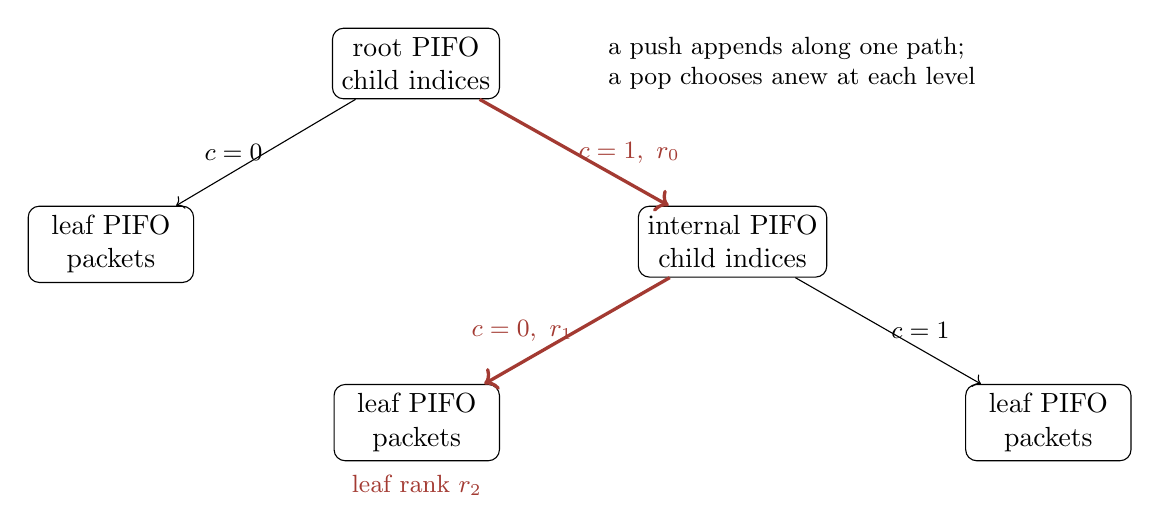
\begin{tikzpicture}[
  q/.style={draw,rounded corners,minimum width=2.1cm,minimum height=.72cm,
            align=center,fill=white},
  every edge/.style={draw,-{Stealth[length=2mm]}},
  lab/.style={font=\small,inner sep=1pt},
  node distance=1.35cm and 1.75cm]
  \node[q] (root) {root PIFO\\child indices};
  \node[q,below left=of root] (left) {leaf PIFO\\packets};
  \node[q,below right=of root] (mid) {internal PIFO\\child indices};
  \node[q,below left=of mid] (mleft) {leaf PIFO\\packets};
  \node[q,below right=of mid] (mright) {leaf PIFO\\packets};
  \draw[->] (root) -- node[lab,left] {$c=0$} (left);
  \draw[->,very thick,pifored] (root) -- node[lab,right] {$c=1,\ r_0$} (mid);
  \draw[->,very thick,pifored] (mid) -- node[lab,left] {$c=0,\ r_1$} (mleft);
  \draw[->] (mid) -- node[lab,right] {$c=1$} (mright);
  \node[lab,pifored,below=.14cm of mleft] {leaf rank $r_2$};
  \node[align=left,anchor=west,font=\small] at ($(root.east)+(1.25,0)$)
    {a push appends along one path;\\a pop chooses anew at each level};
\end{tikzpicture}
\caption{A PIFO-tree state.  Internal entries name children; leaf entries name
packets.  The highlighted annotated path installs ranks \(r_0,r_1,r_2\) with
one shared arrival stamp.  A later pop follows whichever child entry is then
minimal; it need not follow a single source push's path.}
\label{fig:model-tree}
\end{figure}

\subsection{Stateless schedulers and observations}

Fix \(k\in\Nat\) and the finite packet alphabet \(A=\Fin(k)\).  A scheduler is
a topology together with an assignment
\[
  S=(\tau,\mathsf{assign}),
  \qquad \mathsf{assign}:A\to\mathsf{Path}.
\]
It is \emph{valid} when \(\mathsf{assign}(a)\) fits \(\tau\) for every packet
type \(a\).  It is \emph{stateless} because every occurrence of type \(a\)
uses exactly the same annotated path: the same child choices and the same rank
at every level.  The two schedulers compared below may have different
topologies.

An operation is either \(\push(a)\) or \(\popop\).  A run starts from the empty
tree and counter zero.  The \(j\)-th push increments the counter to \(j\) and
uses \(j\) as the arrival stamp.  It emits no observation.  Each pop contributes
exactly one element of \(\mathsf{Option}(A)\): \(\Some(a)\) on success and
\(\None\) on failure.  A failed pop leaves both the tree and arrival counter
unchanged.  Definedness is therefore observable.

The observation records a packet's type, not its source-push identity.  In the
stateless model these observations contain the same ordering information.
Every two occurrences of one type carry equal ranks in every queue they share,
so FIFO tie breaking releases them in their source arrival order.  Hence the
\(i\)-th emitted occurrence of type \(a\) is the \(i\)-th pushed occurrence of
that type.  Relative to a fixed input operation word, the type trace therefore
determines the source-occurrence identity trace.

For a word \(w=a_1\cdots a_n\in A^*\), define its flush operation word by
\begin{equation}
  \flushOps(w)
  =\push(a_1)\cdots\push(a_n)\,\popop^n.
  \label{eq:flush-ops}
\end{equation}
Exactly \(n\) pops suffice: fewer reveal a prefix of the full deterministic
drain, while additional pops append only \(\None\).  Write \(\run(S,o)\) for
the list of pop observations produced by operation word \(o\).

\begin{definition}[The two equivalences]
For valid schedulers \(S,T\) on \(A\),
\begin{align*}
  S\flusheq T
  &\quad\Longleftrightarrow\quad
    \forall w\in A^*.\ 
    \run(S,\flushOps(w))=\run(T,\flushOps(w)),\\
  S\intereq T
  &\quad\Longleftrightarrow\quad
    \forall o\in\mathsf{Op}(A)^*.\ 
    \run(S,o)=\run(T,o).
\end{align*}
\end{definition}

The frozen proposition is the following statement, uniformly over the finite
alphabet size.

\begin{theorem}[Flushes suffice for stateless PIFO trees]
\label{thm:main}
For every \(k\in\Nat\) and all valid stateless schedulers \(S,T\) over
\(\Fin(k)\),
\[
  S\flusheq T \quad\Longrightarrow\quad S\intereq T.
\]
Consequently flush and interleaved equivalence coincide on valid stateless
PIFO trees.
\end{theorem}

The implication from right to left in the final sentence follows immediately
because every \(\flushOps(w)\) is an operation word.  The nontrivial implication
is proved in \autoref{sec:main-proof}.

\subsection{Correspondence with the frozen Lean statement}

\autoref{tab:lean-map} maps the paper notation to the statement's definitions.
The source file is statement-only: its final item is a definition of a
proposition, not a proof of that proposition.

\begin{table}[H]
\centering
\small
\begin{tabularx}{\textwidth}{@{}>{\raggedright\arraybackslash}p{.34\textwidth}
  >{\ttfamily\raggedright\arraybackslash}p{.33\textwidth}
  >{\raggedright\arraybackslash}X@{}}
\toprule
Paper object & \normalfont Lean name & Source lines\\
\midrule
Entry and its three fields & Entry; .val, .rank, .arr & 53--57\\
PIFO contents & Queue & 59--60\\
Strict entry comparison & better & 64--66\\
PIFO pop & qpop & 68--77\\
Tree shape & Topology & 81--86\\
Runtime tree state & Tree & 88--94\\
Empty tree and forest & emptyTree; emptyForest & 96--104\\
Annotated path & Path & 106--113\\
Path well-formedness & pathOk; pathOkAt & 115--126\\
Tree push and list helper & treePush; treePushAt & 128--143\\
Atomic tree pop and list helper & treePop; treePopAt & 145--182\\
Stateless scheduler & Scheduler & 186--193\\
Topology and fixed assignment & Scheduler.topo; Scheduler.assign & 191--192\\
Validity & Scheduler.Valid & 194--197\\
Push/pop operations & Op & 216--220\\
Execution from a state & runFrom & 222--235\\
Execution from the empty state & run & 237--240\\
Flush experiment & flushOps & 244--250\\
Flush equivalence & flushEquiv & 252--254\\
Interleaved equivalence & interEquiv & 256--261\\
Main proposition & statelessFlushImpliesInterleaved & 263--269\\
\bottomrule
\end{tabularx}
\caption{Mathematical-to-Lean correspondence for the frozen formal model.}
\label{tab:lean-map}
\end{table}

% Source pins (SHA-256): PifoStatement.lean=fe9475ebfa2c462d27cb0a99781926074e1281396f2c9e8d32d6dfca788d814e; pifo-elegant-v4.md=356ea38146ced437e20200db04e2ce220c73f9ac9fa892b746f783b8a2d49ab8.
\section{Flushes determine every interleaving}
\label{sec:main-proof}

We prove \autoref{thm:main}.  It is convenient to work over an arbitrary finite
set \(A\); transporting schedulers and operation words along a bijection
\(A\cong\Fin(k)\) gives the frozen statement.

For \(B\subseteq A\), write \(\restrict{w}{B}\) for the subsequence of a word
\(w\) whose letters lie in \(B\).  A natural-valued rank function induces a
total preorder.  For such a preorder \(r\), \(\sort_r(w)\) is the stable sort
of the \emph{occurrences} in \(w\) by
\((r(a),\text{source arrival})\).  For a partition \(P\) of \(A\),
\(\proj{P}(w)\) replaces each letter by its \(P\)-block.  If \(M\) is a
scheduler, \(F_M:A^*\to A^*\) denotes its flush transformer, with the
\(\Some\) constructors erased.  Validity ensures that a flush of \(n\) pushes
has \(n\) successful pops.

\subsection{Operational facts}

The following elementary invariant connects the atomic formal semantics with
the queue-level reasoning used later.

\begin{lemma}[Reference balance]
\label{lem:balance}
At every valid reachable state, for every internal node and each of its
children \(c\),
\begin{equation}
 \#\{\text{queued references to }c\}
 =
 \#\{\text{pending packets in the subtree of }c\}.
 \label{eq:balance}
\end{equation}
Consequently a root pop fails exactly when the total pending-packet count is
zero; after an internal queue selects a child, recursive failure is impossible.
\end{lemma}

\begin{proof}
Initially both sides of \autoref{eq:balance} are zero at every node.  A valid
push through child \(c\) appends exactly one reference to \(c\) and exactly one
packet somewhere below \(c\); it does not affect the equality for another
child.  A successful pop selecting \(c\) removes one such reference and,
recursively, one packet below \(c\).  Induction down the selected path gives a
successful leaf pop.  Hence a positive root count supplies a complete
root-to-leaf pop, while count zero means the root queue is empty.  The atomic
partial-failure branch exists in the definition but is unreachable from a
valid reachable state.
\end{proof}


In particular, for a fixed operation word, the \(\None/\Some\) pattern depends
only on the number of preceding pushes and successful pops, not on ranks or
topology.  Two valid schedulers therefore have identical definedness patterns.

\begin{lemma}[Timestamp compression]
\label{lem:compression}
Replace the arrival stamps occurring in any embedded queue computation by
\(1,2,\ldots\) in their existing strict order.  Every queue selection, and
hence every emitted value, is unchanged.
\end{lemma}

\begin{proof}
Ranks are unchanged.  Equal-rank entries are compared only by the order of
their arrival stamps, which a strictly increasing replacement preserves.
Every choice of a least \((\rank,\arr)\) key is therefore the same.  Induction
over the operation word gives the claim.
\end{proof}

This lemma allows a child invoked at sparse global timestamps to be compared
with a standalone run whose pushes are consecutively stamped.  We will also
attach a ghost source-occurrence tag to every entry when couplings need to
identify an insertion.  The tag is not part of the model and is never
observed; erasing it commutes with every transition because queue ordering uses
only rank and arrival.  Within every reachable queue, and within every abstract
pending-occurrence list used below, arrival stamps are pairwise distinct.  The
same source push may deliberately occur at several selector levels with the
same stamp.  Consequently \((\rank,\arr)\) is a strict key within each
selector: every selection has a unique minimum.  Arrival injectivity is used
in the colored-PIFO coupling, while the strict-key consequence is used in the
diamond and collapse arguments.

\subsection{What two types reveal}

\begin{lemma}[Two-type reduction]
\label{lem:two-type}
For distinct types \(x,y\), the restriction of a stateless PIFO tree to
operation words over \(\{x,y\}\) behaves as one stable PIFO with an effective
comparison
\[
  e(x,y)\in\{x<y,\ x\sim_e y,\ y<x\},
\]
where \(\sim_e\) denotes a rank tie rather than equality of types.
The comparison is determined by the two binary flushes in
\autoref{tab:binary-recovery}.
\end{lemma}

\begin{proof}
Follow the assigned paths of \(x\) and \(y\) together.  Stop at their first
internal node with different child indices, or at their common leaf if their
indices never differ.  At every earlier node all relevant references carry the
same child value.  Such a node forwards one anonymous service for each
successful pop and cannot choose between the two types.

At a decisive internal node, its selected child identifies \(x\) or \(y\), and
the selected child's restricted subtree is monochromatic.  At a decisive leaf,
the queue emits \(x\) or \(y\) directly.  In either case one rank comparison at
this node, with FIFO order on equality, determines every restricted operation
word.  If \(x\) is strictly earlier, both two-letter arrival orders drain as
\(xy\); if the ranks tie, each arrival order is retained; and if \(y\) is
strictly earlier, both drain as \(yx\).  These are exactly the three rows of
\autoref{tab:binary-recovery}.
\end{proof}

\begin{table}[H]
\centering
\begin{tabular}{@{}c@{\qquad}cc@{}}
\toprule
effective comparison \(e(x,y)\) & \(F(xy)\) & \(F(yx)\)\\
\midrule
\(x<y\) & \(xy\) & \(xy\)\\
\(x\sim_e y\) & \(xy\) & \(yx\)\\
\(y<x\) & \(yx\) & \(yx\)\\
\bottomrule
\end{tabular}
\caption{Recovery of the effective binary comparison.  Both arrival orders are
needed to distinguish a rank tie from either strict order.}
\label{tab:binary-recovery}
\end{table}

Notice that \(e(x,y)\) is an extensional fact about the restricted scheduler;
it need not be read from a particular syntactic node.  Flush-equivalent
schedulers have the same \(e\) for every pair by
\autoref{tab:binary-recovery}.

\subsection{A colored-PIFO coupling}

The induction will replace a root preorder while retaining only the sequence
of selected children.  The next lemma justifies that replacement for arbitrary
interleavings, including exact cross-color rank ties.

\begin{lemma}[Colored PIFOs]
\label{lem:colored}
Let \(p,q\) be total preorders on a finite set of types, and let
\(\gamma\) color those types.  Suppose
\begin{equation}
 \gamma(x)\ne\gamma(y)
 \quad\Longrightarrow\quad
 \cmp_p(x,y)=\cmp_q(x,y),
 \label{eq:cross-color-agree}
\end{equation}
where comparison has the three values less, equal, and greater.  PIFO queues
ordered by \(p\) and \(q\), subjected to identical pushes and pops, emit
identical color traces.
\end{lemma}

\begin{proof}
Refine each color into \emph{cross-profile classes}.  Define
\begin{equation}
 x\sim y
 \quad\Longleftrightarrow\quad
 \gamma(x)=\gamma(y)
 \ \land\ 
 \forall z\text{ of another color}.\ 
   \cmp_p(x,z)=\cmp_p(y,z).
 \label{eq:profile-class}
\end{equation}
By \autoref{eq:cross-color-agree}, the same classes are obtained from \(q\).
We use three consequences of totality and transitivity.

First, two distinct classes of one color are strictly separated in the same
direction by both preorders.  Indeed, an outside type witnessing the difference
between their profiles lies weakly on different sides of them; transitivity
rules out reversing that separation.  Second, if a class ties a type of another
color, it is \emph{value-pinned}: every member ties that witness and therefore
all members tie one another, under both \(p\) and \(q\).  Third, comparisons
between differently colored occurrences agree outright by hypothesis.

Couple the two queues while maintaining the following invariant:
\begin{enumerate}
\item every profile class has the same pending count on both sides; and
\item every class that ties another class has literally the same pending list
      of ghost-tagged occurrences on both sides.
\end{enumerate}
The invariant holds initially and identical pushes extend both copies in the
same class.

Consider a pop.  Suppose the \(p\)-queue selects occurrence \(o_1\) in class
\(K_1\), while the \(q\)-queue selects \(o_2\) in a different class \(K_2\).
Equal class counts provide a pending \(K_2\)-occurrence on the \(p\)-side and a
pending \(K_1\)-occurrence on the \(q\)-side.  Minimality of the selected
entries implies, member-wise,
\[
  K_1\le_p K_2
  \qquad\text{and}\qquad
  K_2\le_q K_1.
\]
The classes cannot have one color: their strict, same-direction separation
would contradict these inequalities.  They have different colors, so their
constant cross-class comparison is common to \(p\) and \(q\).  The two
inequalities force that comparison to be a tie in both directions.

Both classes are therefore value-pinned.  By the invariant, each class's
pending occurrence list is identical across the queues.  Thus \(o_1\) and
\(o_2\) are pending in both queues, and their rank components tie within each
queue.  Minimality on the \(p\)-side gives
\(\arr(o_1)\le\arr(o_2)\); minimality on the \(q\)-side gives the reverse, so
the stamps are equal.  Both occurrences lie in each queue, where arrival
stamps are injective, hence \(o_1=o_2\), contradicting \(K_1\ne K_2\).

Both pops therefore select one profile class and emit the same color.  Its
pending count decreases on both sides.  If the class ties another class, it is
value-pinned, so both queues remove its arrival-least pending occurrence---the
same occurrence---and the identical-list clause survives.  Other lists are
untouched.  Empty pops agree because total pending counts agree.  Induction on
the common operation word completes the coupling.
\end{proof}

% Source pin (SHA-256): pifo-elegant-v4.md=356ea38146ced437e20200db04e2ce220c73f9ac9fa892b746f783b8a2d49ab8.
\subsection{Proper flush decompositions}
\label{sec:decompositions}

For induction on the alphabet, we expose the first queue that makes a
nontrivial routing decision.

\begin{lemma}[Proper top decomposition]
\label{lem:decomposition}
If \(|A|>1\), every valid stateless scheduler is online-equivalent to a
scheduler of the form
\begin{equation}
 M=(P,r,(M_B)_{B\in P}),
 \label{eq:decomposition-shape}
\end{equation}
where \(P\) is a proper partition of \(A\) into active root children, \(r\) is
the total preorder induced by root ranks, and \(M_B\) is the child scheduler
restricted to types in \(B\).  Its flush transformer satisfies
\begin{align}
 \restrict{F_M(w)}{B}
   &=F_{M_B}(\restrict{w}{B})
    =F_M(\restrict{w}{B}),
    \label{eq:block-projection}\\
 \proj{P}(F_M(w))
   &=\proj{P}(\sort_r(w)).
    \label{eq:root-pattern}
\end{align}
\end{lemma}

\begin{proof}
Starting at the root, follow the unique active child used by all types for as
long as one exists.  Each skipped queue contains only that child value and
therefore forwards exactly one service per successful pop; removing such a
node preserves every online trace.  The walk ends either at the first node with
at least two active children or at a leaf.  In the former case, partition types
by the chosen child.  Every block is nonempty and, because at least two are
active, proper.

In the leaf case, replace the leaf by an internal root having the old leaf rank
for each type and one FIFO singleton child per type.  The new root queue mirrors
the old leaf queue occurrence-for-occurrence, while a singleton child has no
choice to make.  Since \(|A|>1\), the singleton partition is proper.  This
establishes \autoref{eq:decomposition-shape} without changing online behavior.

During a flush, child \(B\) receives all pushes in
\(\restrict{w}{B}\) before it receives service, and the root calls it exactly
\(|\restrict{w}{B}|\) times.  Its complete output is therefore
\(F_{M_B}(\restrict{w}{B})\), proving the first equality of
\autoref{eq:block-projection}.  On a word confined to \(B\), all root references
select \(B\), which proves the second.  Finally the root drains its reference
occurrences by the stable \((r,\arr)\) order.  Replacing their source types by
their child blocks yields \autoref{eq:root-pattern}.
\end{proof}

We call \((P,r)\) a \emph{decomposition} of a word transformer \(F\) when
\autoref{eq:block-projection} and \autoref{eq:root-pattern} hold.  Two consequences will be used
without further comment:
\begin{align}
  F(v)&=F_{M_B}(v) &&\text{if every letter of \(v\) lies in \(B\)},
  \label{eq:block-autonomy-simple}\\
  \restrict{F(w)}{B}&=F(\restrict{w}{B}) &&\text{for arbitrary \(w\)}.
  \label{eq:block-filter-simple}
\end{align}
The first is \emph{block autonomy}; the second says that deleting other blocks
commutes with the transformer.

\subsection{Combining two decompositions}
\label{sec:meet}

Suppose \((P,r)\) and \((Q,s)\) decompose one common flush transformer \(F\).
Their meet partition is the set of nonempty incidence cells
\begin{equation}
 R=P\wedge Q
  =\{B\cap C\ne\varnothing:B\in P,\ C\in Q\}.
 \label{eq:meet-partition}
\end{equation}
We will construct a total preorder that agrees with \(r\) across \(P\)-blocks
and with \(s\) across \(Q\)-blocks.  We do \emph{not} need to claim that the
resulting pair \((R,t)\) itself decomposes \(F\).

First, every cell inherits autonomy.  For \(D=B\cap C\), repeated use of
\autoref{eq:block-filter-simple} gives
\begin{equation}
\begin{aligned}
 \restrict{F(w)}{D}
 &=\restrict{(\restrict{F(w)}{B})}{C}
  =\restrict{F(\restrict{w}{B})}{C}\\
 &=F(\restrict{(\restrict{w}{B})}{C})
  =F(\restrict{w}{D}).
\end{aligned}
\label{eq:cell-autonomy}
\end{equation}

For types in distinct \(R\)-cells, prescribe the effective comparison
\(e(x,y)\) recovered by \lemref{lem:two-type}.  If \(P\) separates the pair, its
two-type restriction is chosen at the \(P\)-root, and therefore
\begin{equation}
 e(x,y)=\cmp_r(x,y).
 \label{eq:e-from-r}
\end{equation}
Likewise, if \(Q\) separates it,
\begin{equation}
 e(x,y)=\cmp_s(x,y).
 \label{eq:e-from-s}
\end{equation}
The prescriptions agree when both partitions separate the pair because both
are recovered from the same two flushes of \(F\).

\begin{figure}[t]
\centering
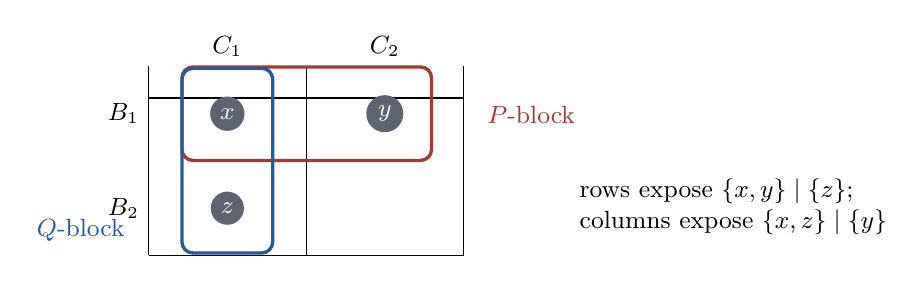
\begin{tikzpicture}[
  cell/.style={minimum width=2.0cm,minimum height=1.2cm,draw},
  pt/.style={circle,fill=pifogray,text=white,inner sep=2.1pt,font=\small},
  every node/.style={font=\small}]
  \draw[step=2cm] (0,0) grid (4,2.4);
  \node[pt] (x) at (1,1.8) {$x$};
  \node[pt] (y) at (3,1.8) {$y$};
  \node[pt] (z) at (1,.6) {$z$};
  \node[above] at (1,2.4) {$C_1$};
  \node[above] at (3,2.4) {$C_2$};
  \node[left] at (0,1.8) {$B_1$};
  \node[left] at (0,.6) {$B_2$};
  \node[draw=pifored,very thick,rounded corners,fit=(x)(y),inner sep=10pt] {};
  \node[draw=pifoblue,very thick,rounded corners,fit=(x)(z),inner sep=10pt] {};
  \node[pifored,anchor=west] at (4.18,1.78) {$P$-block};
  \node[pifoblue,anchor=east] at (-.18,.32) {$Q$-block};
  \node[align=left,anchor=west] at (5.35,.62)
    {rows expose $\{x,y\}\mid\{z\}$;\\
     columns expose $\{x,z\}\mid\{y\}$};
\end{tikzpicture}
\caption{The only nontrivial three-cell incidence shape.  Three meet cells
form an L when neither all \(P\)-coordinates nor all \(Q\)-coordinates are
distinct.  Its two visible decompositions form the diamond used below.}
\label{fig:meet-diamond}
\end{figure}

\begin{lemma}[Three-cell diamond]
\label{lem:diamond}
On one representative type from each of any three distinct meet cells, the
pairwise comparisons \(e\) form a total preorder.
\end{lemma}

\begin{proof}
View the cells as occupied positions in the \(P\times Q\) incidence grid.  If
the three \(P\)-coordinates are distinct, all comparisons come from the genuine
preorder \(r\) by \autoref{eq:e-from-r}.  If their \(Q\)-coordinates are distinct,
they all come from \(s\) by \autoref{eq:e-from-s}.  Otherwise the three positions
form an L as in \autoref{fig:meet-diamond}; naming its corner \(x\), the restricted
transformer has both decompositions
\begin{equation}
  \{x,y\}\mid\{z\},
  \qquad
  \{x,z\}\mid\{y\}.
  \label{eq:l-decompositions}
\end{equation}

Assume that the non-strict relation induced by \(e\) is not transitive.  Since
each pair is totally compared, there are distinct \(a,b,c\) with
\begin{equation}
  a\le_e b,
  \qquad b\le_e c,
  \qquad c<_e a.
  \label{eq:bad-triple}
\end{equation}
Push one occurrence of each in the cycle order \(a,b,c\), then flush.  The
arrival stamps are distinct, so every queue computation has a unique least
\((\rank,\arr)\) key.  The cycle inequalities determine every strict or weak
root comparison, and the fixed arrival order resolves any remaining rank tie;
no separate tie case split is needed.

Consider in full the L orientation whose grouped pairs are \(\{b,c\}\) and
\(\{c,a\}\).  In the decomposition
\(\{b,c\}\mid\{a\}\), separated-pair comparisons give root ranks
\(\rho_a\le\rho_b\) and \(\rho_c<\rho_a\).  Thus
\(\rho_c<\rho_b\), and the root drains references in the order
\(c,a,b\): if \(\rho_a=\rho_b\), arrival puts \(a\) first.  The resulting
child slots are
\[
  \{b,c\},\ a,\ \{b,c\}.
\]
Within the pair child, \(b\) arrived before \(c\) and \(b\le_e c\), so the
binary recovery table says that its output is \(b,c\).  The complete output is
therefore \(b,a,c\).

In the decomposition \(\{c,a\}\mid\{b\}\), separated comparisons give
\(\sigma_a\le\sigma_b\le\sigma_c\).  With arrival order \(a,b,c\), the root
drains references in that same order, producing slots
\[
  \{c,a\},\ b,\ \{c,a\}.
\]
The pair child outputs \(c,a\), since \(c<_e a\), and the complete output is
\(c,b,a\).  The first letters differ, contradicting that both decompositions
compute the same \(F(abc)\).

Cyclic renaming covers the other two placements of the two grouped edges in
the comparison cycle.  Exchanging the roles of the two decompositions covers
the three reflected L orientations.  These exhaust the incidence shape, so no
failure of transitivity is possible.  Reflexivity and totality are already
built into the pair comparisons; hence the restriction is a total preorder.
\end{proof}

\begin{figure}[t]
\centering
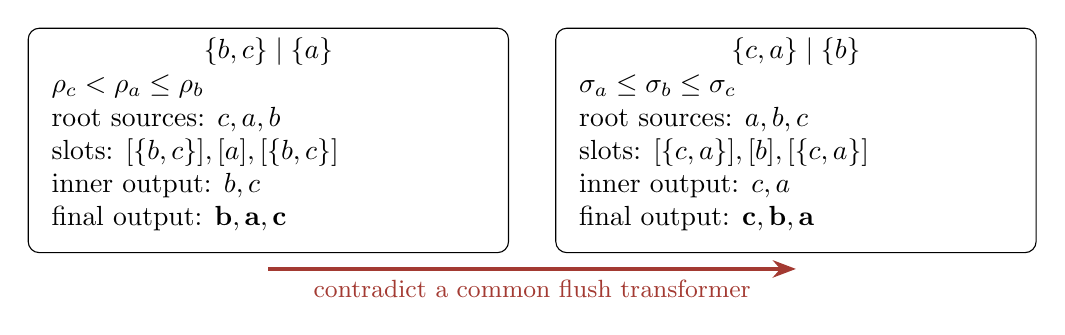
\begin{tikzpicture}[
  panel/.style={draw,rounded corners,minimum width=6.1cm,minimum height=2.85cm,
                align=left,inner sep=8pt},
  title/.style={font=\bfseries}]
  \node[panel] (l) at (-3.35,0) {};
  \node[title,anchor=north] at (l.north) {$\{b,c\}\mid\{a\}$};
  \node[align=left,anchor=north west] at ($(l.north west)+(.18,-.48)$)
    {$\rho_c<\rho_a\le\rho_b$\\
     root sources: $c,a,b$\\
     slots: $[\{b,c\}], [a], [\{b,c\}]$\\
     inner output: $b,c$\\
     final output: $\mathbf{b,a,c}$};
  \node[panel] (r) at (3.35,0) {};
  \node[title,anchor=north] at (r.north) {$\{c,a\}\mid\{b\}$};
  \node[align=left,anchor=north west] at ($(r.north west)+(.18,-.48)$)
    {$\sigma_a\le\sigma_b\le\sigma_c$\\
     root sources: $a,b,c$\\
     slots: $[\{c,a\}], [b], [\{c,a\}]$\\
     inner output: $c,a$\\
     final output: $\mathbf{c,b,a}$};
  \draw[-{Stealth},very thick,pifored] ($(l.south)+(0,-.2)$) --
    node[below,font=\small] {contradict a common flush transformer}
    ($(r.south)+(0,-.2)$);
\end{tikzpicture}
\caption{The representative diamond computation for
\(a\le_e b\le_e c<_e a\), using one common arrival order \(a,b,c\).
Internal references choose child slots; the selected pair child may emit a
different source occurrence.}
\label{fig:diamond-computation}
\end{figure}


The diamond controls triples of cells.  The next argument shows that no
higher-arity obstruction remains.

\begin{lemma}[Meet-compatible preorder]
\label{lem:meet-preorder}
If \((P,r)\) and \((Q,s)\) decompose \(F\), there is a natural-valued total
preorder \(t\) such that
\begin{equation}
 \begin{aligned}
  \cmp_t(x,y)&=\cmp_r(x,y)
    &&\text{whenever \(x,y\) lie in distinct \(P\)-blocks},\\
  \cmp_t(x,y)&=\cmp_s(x,y)
    &&\text{whenever \(x,y\) lie in distinct \(Q\)-blocks}.
 \end{aligned}
 \label{eq:meet-compatibility}
\end{equation}
\end{lemma}

\begin{proof}
Build a directed constraint graph on the types.  Between distinct meet cells,
each relation \(x\le_e y\) contributes a weak edge \(x\to y\), marked exactly
when \(x<_e y\).  Thus a preorder tie contributes unmarked edges in both
directions.  It is enough to prove that no directed cycle contains a marked
edge.

Suppose otherwise.  Choose a marked edge \(a\to b\) as the head of such a
cycle and argue by strong induction on its length.  Let \(c,d\) be the next
vertices after \(b\) when present.  Only the three fixed chord positions
\((a,c)\), \((b,d)\), and \((a,d)\) are needed; they are shown in
\autoref{fig:fixed-chords}.

For length two, the return edge \(b\to a\) contradicts the strict comparison
on the marked head.  For length three, the consecutive edges join three
distinct cells, and \lemref{lem:diamond} supplies a genuine total preorder on
the triple; such a preorder cannot contain a marked directed triangle.

Consider a length-four cycle \((a,b,c,d)\).  If \(a\) and \(c\) occupy
distinct cells, compare that chord.  An edge \(c\to a\) closes the marked
triangle \(a\to b\to c\to a\).  Otherwise totality gives \(a\to c\), and it
is marked: in the three-cell preorder, \(a<_e b\le_e c\) implies
\(a<_e c\).  The cycle \(a\to c\to d\to a\) is then a marked triangle.
Likewise, if \(b,d\) occupy distinct cells, an edge \(b\to d\) yields the
marked triangle \(a\to b\to d\to a\), which retains the original marked
head; if that edge is unavailable, totality makes \(d\to b\) strict, yielding
the marked triangle \(b\to c\to d\to b\).  If both diagonals are intra-cell,
the cycle alternates between two meet cells.
All four cross-cell comparisons then come from one genuine preorder: from
\(r\) when \(P\) separates those cells, and otherwise from \(s\), since \(Q\)
must separate them.  Its ranks would have to satisfy
\[
 \rho_a\le\rho_b\le\rho_c\le\rho_d\le\rho_a
 \quad\text{while}\quad
 \rho_b\le\rho_a\text{ is false},
\]
which is impossible.

Now let the length be at least five.  If \(a,c\) lie in distinct cells, an
edge \(c\to a\) closes the marked triangle through \(a,b,c\).  Otherwise the
forward chord \(a\to c\) is strict by the same three-cell argument, and
replacing \(a\to b\to c\) by this marked head shortens the cycle.  Strong
induction excludes it.

We may therefore assume \(a,c\) are in one cell.  If \(b,d\) are in distinct
cells and the forward edge \(b\to d\) exists, replacing
\(b\to c\to d\) by it shortens the cycle while retaining the original marked
head \(a\to b\).  If the forward edge is unavailable, totality makes the
reverse edge \(d\to b\) strict, closing a marked triangle through \(b,c,d\).
Thus \(b,d\) must also be in one cell.

Now \(a,d\) lie in distinct cells: otherwise \(a,c,d\) would share a cell,
contradicting the cross-cell edge \(c\to d\).  If the chord \(d\to a\) exists,
it closes the already excluded length-four marked cycle
\(a\to b\to c\to d\to a\).  In the other orientation, all four cross-cell
comparisons come from one original root preorder because \(a,c\) share one
cell and \(b,d\) share another.  In that preorder,
\(a<_e b\le_e c\le_e d\), so \(a\to d\) is strict.  Replacing the three-edge
prefix by this marked head produces a shorter marked cycle.  Strong induction
excludes every case, so no marked cycle exists.

It remains to realize all constraints by natural ranks.  Write \(z\leadsto x\)
for reflexive graph reachability, allowing a path of length zero, and set
\begin{equation}
 t(x)=
 \#\{z:z\leadsto x\ \land\ x\not\leadsto z\}.
 \label{eq:counting-linearization}
\end{equation}
Let \(L_x=\{z:z\leadsto x\land x\not\leadsto z\}\).  If \(x\to y\) is a weak
edge and \(z\in L_x\), then \(z\leadsto x\to y\).  A return path
\(y\leadsto z\) would imply \(x\leadsto z\), a contradiction; hence
\(z\in L_y\), and \(L_x\subseteq L_y\).  If \(x\to y\) is marked, no path
returns from \(y\) to \(x\), since it would complete a marked cycle.  Thus
\(x\in L_y\), whereas reflexivity gives \(x\notin L_x\).  The inclusion is
strict and finiteness gives \(t(x)<t(y)\).  A prescribed tie contributes weak
edges both ways, so the two inclusions give equal predecessor sets and equal
ranks.  Thus \(t\) realizes every prescribed \(e\)-comparison.  The constraints in
\autoref{eq:e-from-r} and \autoref{eq:e-from-s} give exactly
\autoref{eq:meet-compatibility}.
\end{proof}

\begin{figure}[t]
\centering
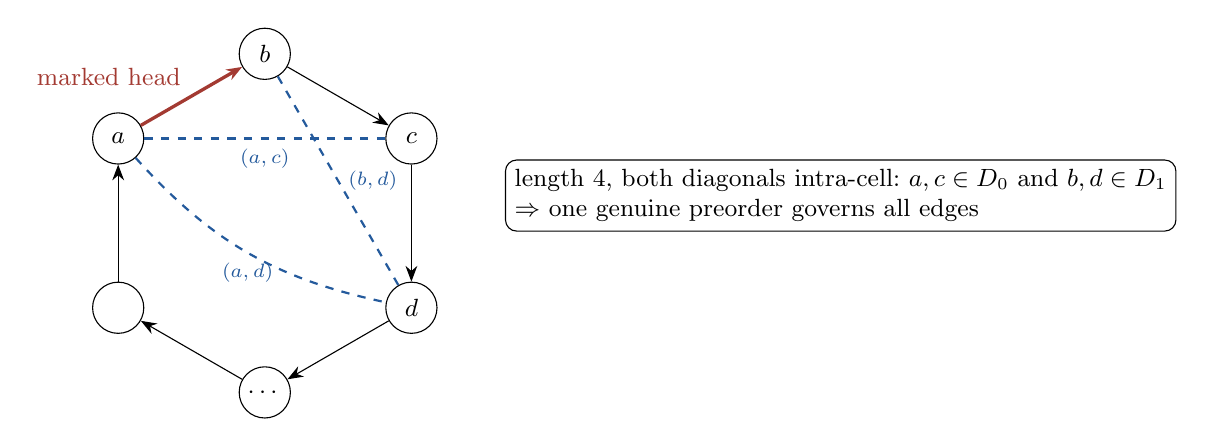
\begin{tikzpicture}[
  v/.style={circle,draw,minimum size=6.5mm,inner sep=0pt,font=\small},
  arr/.style={-{Stealth[length=2mm]}},
  chord/.style={dashed,pifoblue,thick}]
  \node[v] (a) at (150:2.15) {$a$};
  \node[v] (b) at (90:2.15) {$b$};
  \node[v] (c) at (30:2.15) {$c$};
  \node[v] (d) at (-30:2.15) {$d$};
  \node[v] (e) at (-90:2.15) {$\cdots$};
  \node[v] (f) at (-150:2.15) {};
  \draw[arr,very thick,pifored] (a) -- node[above left,font=\small,
    text=pifored] {marked head} (b);
  \draw[arr] (b) -- (c);
  \draw[arr] (c) -- (d);
  \draw[arr] (d) -- (e);
  \draw[arr] (e) -- (f);
  \draw[arr] (f) -- (a);
  \draw[chord] (a) -- node[below,font=\scriptsize] {$(a,c)$} (c);
  \draw[chord] (b) -- node[right,font=\scriptsize] {$(b,d)$} (d);
  \draw[chord] (a) to[bend right=18]
    node[below,font=\scriptsize] {$(a,d)$} (d);
  \node[draw,rounded corners,align=left,font=\small,anchor=west]
    at (3.05,.35) {length $4$, both diagonals intra-cell:\
      $a,c\in D_0$ and $b,d\in D_1$\\
      $\Rightarrow$ one genuine preorder governs all edges};
\end{tikzpicture}
\caption{The fixed-head-chord induction.  A longer marked cycle is shortened
or reduced to a three-cell diamond using only the displayed chord positions;
the alternating length-four case is controlled by one original root preorder.}
\label{fig:fixed-chords}
\end{figure}

\subsection{Strong induction: swap, refine, and collapse}
\label{sec:induction}

We now prove \autoref{thm:main} simultaneously for every finite alphabet by
strong induction on \(|A|\).  If \(A\) is empty, every operation is a failed
pop.  If \(|A|=1\), each successful pop emits the sole type, and
\lemref{lem:balance} says that success is determined only by the push/pop count.

Assume \(|A|>1\), and let \(S,T\) be flush-equivalent valid stateless
schedulers.  By \lemref{lem:decomposition}, normalize them online to proper top
decompositions
\begin{equation}
  S=(P,r,(S_B)_{B\in P}),
  \qquad
  T=(Q,s,(T_C)_{C\in Q}),
  \label{eq:two-top-decompositions}
\end{equation}
with common flush transformer \(F\).  Form \(R=P\wedge Q\) and choose the
meet-compatible preorder \(t\) from \lemref{lem:meet-preorder}.

\paragraph{Swap before refining.}
Replace \(S\)'s root order \(r\) by \(t\), leaving its partition and children
unchanged.  Across distinct \(P\)-blocks the two root preorders agree by
\autoref{eq:meet-compatibility}.  Apply \lemref{lem:colored} with colors \(P\).
The root has the same complete online \(P\)-token trace, so every child receives
the same driven word.  Thus
\begin{equation}
  S\intereq S^t
  \qquad\text{and}\qquad
  F_{S^t}=F.
  \label{eq:s-root-swap}
\end{equation}
Symmetrically \(T\intereq T^t\).  Applying
\autoref{eq:root-pattern} directly to the two swapped schedulers gives both pattern
facts, for every \(w\),
\begin{equation}
 \proj{P}(F(w))=\proj{P}(\sort_t(w)),
 \qquad
 \proj{Q}(F(w))=\proj{Q}(\sort_t(w)).
 \label{eq:both-patterns}
\end{equation}
This order of operations is important: after the swaps, no separate meet-cell
control-word construction is needed.

\paragraph{Refine one proper block.}
For every meet cell \(D\in R\), choose a valid scheduler \(U_D\) realizing the
restricted transformer \(F\) on \(D\).  For example, restrict \(S\)'s fixed
assignment to types in \(D\); cell autonomy
\autoref{eq:cell-autonomy} identifies its flush transformer with
\(\restrict{F}{D}\).

Fix \(B\in P\).  Let \(V_B\) have a \(t\)-ordered root routing to the nonempty
cells \(D=B\cap C\) below \(B\), with child \(U_D\) at cell \(D\).  We claim
\begin{equation}
  F_{S_B}=F_{V_B}.
  \label{eq:block-flush-equality}
\end{equation}
Take a word \(v\) over \(B\).  A word over \(B\) is uniquely reconstructed
from its \(Q\)-block pattern and its subsequence in every \(Q\)-block.  By block
autonomy, \(F_{S_B}(v)=F(v)\), whose \(Q\)-pattern is
\(\proj{Q}(\sort_t(v))\) by \autoref{eq:both-patterns}.  The root-pattern equation
for \(V_B\) gives the same pattern.

Fix a block \(C\in Q\) and set \(D=B\cap C\).  If \(D=\varnothing\), both
\(C\)-subsequences are empty because both output words lie in \(B\).  If
\(D\ne\varnothing\), then \(D\in R\), so \(U_D\) is defined.  Because \(v\)
is a \(B\)-word, \(\restrict{v}{C}=\restrict{v}{D}\), and
\begin{equation}
\begin{aligned}
 \restrict{F(v)}{C}
 &=F(\restrict{v}{C})
  =F(\restrict{v}{D})\\
 &=F_{U_D}(\restrict{v}{D})
  =\restrict{F_{V_B}(v)}{C}.
\end{aligned}
\label{eq:block-subsequences}
\end{equation}
Here the first equality is autonomy for the \(Q\)-decomposition, the third is
the choice of \(U_D\), and the last is
\autoref{eq:block-projection} for \(V_B\); filtering by \(C\) and by \(D\) agrees
because every output of \(V_B\) lies in \(B\).  Equal pattern and equal
subsequences prove \autoref{eq:block-flush-equality}.

The partition \(P\) is proper, so \(|B|<|A|\).  The induction hypothesis
applied to \autoref{eq:block-flush-equality} gives
\begin{equation}
  S_B\intereq V_B.
  \label{eq:block-inter-equality}
\end{equation}
Substitute \(V_B\) for every child \(S_B\) under the already swapped
\(t\)-root.  The root reference queue is unchanged.  Child \(B\) receives its
projected pushes and one anonymous pop whenever a \(B\)-token is selected, so
the driven operation word is the same on both sides.  Its global arrival stamps
may have gaps; \lemref{lem:compression} converts them monotonically to the
standalone instance of \autoref{eq:block-inter-equality}.  Child substitution
therefore preserves the entire online trace.

\paragraph{Collapse equal selector levels.}
After substitution, the scheduler has two routing levels: an outer root over
the \(P\)-blocks and, inside each \(B\), a root over its \(R\)-cells.  Both
levels use preorder \(t\).  Let \(U\) instead have one \(t\)-root routing
directly to the same children \(U_D\).

Couple these schedulers with a set \(\Omega\) of pending ghost-tagged
selector-reference occurrences.  Maintain:
\begin{enumerate}
\item the two-level outer queue is \(\Omega\), labeled by \(P\)-block;
\item \(U\)'s root queue is \(\Omega\), labeled by \(R\)-cell;
\item the inner queue below \(B\) is \(\restrict{\Omega}{B}\), labeled by
      \(R\)-cell; and
\item corresponding \(U_D\) states are identical.
\end{enumerate}
Pushes extend exactly the corresponding queues and child state.  On a pop, let
the outer queue select occurrence \(o\in B\).  Every selector uses the same key
\((t,\arr)\), and arrival stamps within \(\Omega\) are pairwise distinct, so
\(o\) is the unique minimum of \(\Omega\) and therefore also of
\(\restrict{\Omega}{B}\).  The inner queue selects the same occurrence; the
one-level root, holding the same \(\Omega\) with the same keys, also selects
\(o\).  There is no full-key tie case.  Both sides call the same \(U_D\) state.
A successful lower pop removes \(o\) from all corresponding selectors.  An
atomic lower failure rolls both sides back identically.  The invariant
survives, and
\begin{equation}
  S\intereq U.
  \label{eq:s-to-u}
\end{equation}

Starting from \(T\), swap its root to \(t\), refine each proper
\(C\in Q\) into a \(t\)-root over the same meet-cell schedulers \(U_D\), and
collapse.  The proof of block flush equality is the mirror image of
\autoref{eq:block-flush-equality}: use the \(P\)-pattern in
\autoref{eq:both-patterns} and autonomy from the \(S\)-side.  It gives
\begin{equation}
  T\intereq U.
  \label{eq:t-to-u}
\end{equation}
Transitivity of equality of run outputs yields \(S\intereq T\).  The argument
has coupled successful outputs; \lemref{lem:balance} restores the identical
\(\None\) positions for over-pops.  This proves \autoref{thm:main}.

\begin{figure}[t]
\centering
\resizebox{.98\textwidth}{!}{%
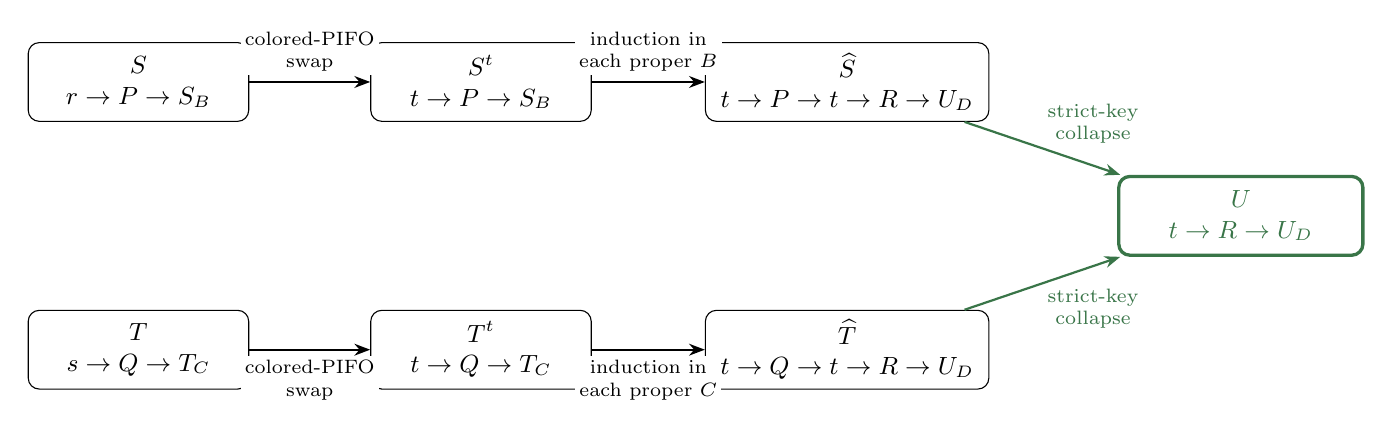
\begin{tikzpicture}[
  box/.style={draw,rounded corners,align=center,minimum width=2.8cm,
              minimum height=1.0cm,font=\small},
  arr/.style={-{Stealth[length=2mm]},thick},
  lab/.style={font=\scriptsize,align=center,fill=white,inner sep=1.5pt}]
  \node[box] (s) at (0,1.7) {$S$\\$r\to P\to S_B$};
  \node[box] (st) at (4.35,1.7) {$S^t$\\$t\to P\to S_B$};
  \node[box,minimum width=3.6cm] (sr) at (9.0,1.7)
    {$\widehat S$\\$t\to P\to t\to R\to U_D$};
  \node[box] (t0) at (0,-1.7) {$T$\\$s\to Q\to T_C$};
  \node[box] (tt) at (4.35,-1.7) {$T^t$\\$t\to Q\to T_C$};
  \node[box,minimum width=3.6cm] (tr) at (9.0,-1.7)
    {$\widehat T$\\$t\to Q\to t\to R\to U_D$};
  \node[box,minimum width=3.1cm,very thick,pifogreen] (u) at (14.0,0)
    {$U$\\$t\to R\to U_D$};
  \draw[arr] (s) -- node[lab,above=2pt] {colored-PIFO\\swap} (st);
  \draw[arr] (st) -- node[lab,above=2pt] {induction in\\each proper $B$} (sr);
  \draw[arr,pifogreen] (sr) -- node[lab,above right] {strict-key\\collapse} (u);
  \draw[arr] (t0) -- node[lab,below=2pt] {colored-PIFO\\swap} (tt);
  \draw[arr] (tt) -- node[lab,below=2pt] {induction in\\each proper $C$} (tr);
  \draw[arr,pifogreen] (tr) -- node[lab,below right] {strict-key\\collapse} (u);
\end{tikzpicture}%
}
\caption{Proof architecture.  The common preorder \(t\) is installed before
the children are refined.  Strong induction produces the same meet-cell
children on both sides, and identical selector levels collapse to one common
scheduler \(U\).}
\label{fig:proof-architecture}
\end{figure}

\paragraph{Why the induction is well founded.}
Only the original blocks \(B\in P\) and \(C\in Q\) are recursive arguments,
and both top partitions are proper.  A meet cell may equal an entire original
block, and \(V_B\) may consequently have just one active cell, but the measure
is still \(|B|<|A|\), not tree height or the size of an introduced child.
Repeated packet types cause no problem: every projection, stable sort, and
reconstruction above is a computation on occurrences.

% Source pins (SHA-256): PifoStatement.lean=fe9475ebfa2c462d27cb0a99781926074e1281396f2c9e8d32d6dfca788d814e; pifo-verify-all/VERIFICATION.md=c97ed5daa11c97f71a5d0e3867f96ddabe74438f1f598c049050c735a96b1887 (artifact audit; the universal calculation is proved below).
\section{A stateful separation}
\label{sec:stateful}

The fixed type-to-path assignment in \autoref{thm:main} is essential.  We now
work through two flat three-leaf trees whose assignment may inspect the
persistent arrival counter.  They agree on every flush word but disagree on a
five-operation interleaving.

For this example only, let a transaction for push number \(j\) choose a triple
\[
  \mathsf{tx}(j)=(\text{leaf},\text{leaf rank},\text{root rank}).
\]
The choice is independent of the packet label but depends on \(j\).  A pop does
not reset the arrival counter.  In \autoref{tab:stateful-assignments}, notation
\(C(1,1)\) means leaf \(C\), leaf rank \(1\), root rank \(1\).

\begin{table}[H]
\centering
\begin{tabular}{@{}c@{\qquad}l@{\qquad}l@{}}
\toprule
push number & scheduler \(S_1\) & scheduler \(S_2\)\\
\midrule
\(1\) & \(C(1,1)\) & \(E(1,3)\)\\
\(2\) & \(B(1,3)\) & \(E(2,1)\)\\
\(3\) & \(C(2,2)\) & \(F(1,2)\)\\
\(j\ge4\) & \(G(j,100+j)\) & \(G(j,100+j)\)\\
\bottomrule
\end{tabular}
\caption{Arrival-dependent assignments for the counterexample.  Leaf names
are local to a scheduler; both trees have three leaves.}
\label{tab:stateful-assignments}
\end{table}

\begin{proposition}[Stateful flush/interleaving separation]
\label{prop:stateful-separation}
The schedulers in \autoref{tab:stateful-assignments} have identical flush output
for every finite packet word.  They are not interleaved-equivalent.
\end{proposition}

\begin{proof}
First label packet occurrences by their source arrival numbers.  After pushes
\(1,2,3\), scheduler \(S_1\)'s root priority order is
\[
  C_1,\ C_3,\ B_2,
\]
because the respective root ranks are \(1,2,3\).  Leaf \(C\) contains
occurrences \(1,3\) at leaf ranks \(1,2\), while \(B\) contains occurrence
\(2\).  The drain is therefore \(1,3,2\).

Scheduler \(S_2\)'s root priority order is instead
\[
  E_2,\ F_3,\ E_1.
\]
Leaf \(E\) contains occurrence \(1\) at rank \(1\) and occurrence \(2\) at
rank \(2\); \(F\) contains occurrence \(3\).  The first root reference,
\(E_2\), selects leaf \(E\), but that leaf emits occurrence \(1\), not the
occurrence that created the root reference.  Then \(F\) emits \(3\), and the
last \(E\)-service emits \(2\).  The drain is again \(1,3,2\).  This is the
indirection visible in \autoref{fig:counterexample-hijack}.

For \(j\ge4\), both schedulers insert into the common tail leaf \(G\), with
root ranks \(100+j\) and leaf ranks \(j\).  These entries follow the first
three and are ordered increasingly, so both append \(4,5,\ldots,n\).  Directly
checking the shorter prefixes gives
\begin{equation}
 \begin{array}{c|c}
 n & \text{identity drain}\ \\
 \hline
 0 & \epsilon\\
 1 & 1\\
 2 & 1,2\\
 n\ge3 & 1,3,2,4,5,\ldots,n.
 \end{array}
 \label{eq:stateful-flush-pattern}
\end{equation}
Now take an arbitrary label word \(x_1\cdots x_n\).  The transactions ignore
labels, so replacing each identity in \autoref{eq:stateful-flush-pattern} by its
source label shows that both schedulers return
\(x_1x_3x_2x_4\cdots x_n\), with the displayed short cases.  Thus they agree
on every flush word, not merely on words with distinct labels.

For the interleaving
\begin{equation}
  \push;\ \popop;\ \push;\ \push;\ \popop,
  \label{eq:diverging-ops}
\end{equation}
the first push/pop emits occurrence \(1\) and empties both trees, but leaves
the counter at one.  Scheduler \(S_1\) then inserts occurrence \(2\) into
\(B\) at root rank \(3\) and occurrence \(3\) into \(C\) at root rank \(2\),
so the final pop emits \(3\).  Scheduler \(S_2\) inserts occurrence \(2\) into
\(E\) at root rank \(1\) and occurrence \(3\) into \(F\) at root rank \(2\).
The old rank-\(1\) packet in \(E\) is gone; the selected \(E\) leaf therefore
emits occurrence \(2\).  The identity traces are \(1,3\) and \(1,2\).

This is observable with a two-type alphabet.  Choose labels
\(x_1=0,x_2=0,x_3=1\).  The operation word
\(\push(0);\popop;\push(0);\push(1);\popop\) produces type traces
\(0,1\) for \(S_1\) and \(0,0\) for \(S_2\).  Hence interleaved equivalence
fails.
\end{proof}

\begin{figure}[t]
\centering
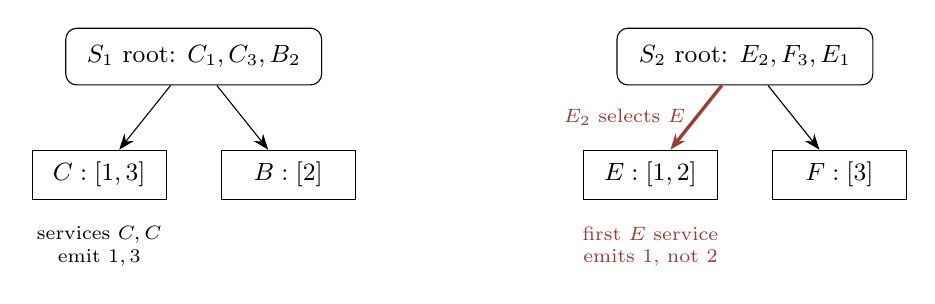
\begin{tikzpicture}[
  q/.style={draw,rounded corners,minimum width=3.25cm,minimum height=.72cm,
            align=center,font=\small},
  leaf/.style={draw,minimum width=1.7cm,minimum height=.62cm,font=\small},
  arr/.style={-{Stealth[length=2mm]}},
  note/.style={font=\scriptsize,align=center}]
  \node[q] (r1) at (-3.5,1.5) {$S_1$ root: $C_1,C_3,B_2$};
  \node[leaf] (c) at (-4.7,0) {$C:[1,3]$};
  \node[leaf] (b) at (-2.3,0) {$B:[2]$};
  \draw[arr] (r1) -- (c);
  \draw[arr] (r1) -- (b);
  \node[note,below=.22cm of c] {services $C,C$\\emit $1,3$};
  \node[q] (r2) at (3.5,1.5) {$S_2$ root: $E_2,F_3,E_1$};
  \node[leaf] (e) at (2.3,0) {$E:[1,2]$};
  \node[leaf] (f) at (4.7,0) {$F:[3]$};
  \draw[arr,very thick,pifored] (r2) --
    node[left,note,text=pifored] {$E_2$ selects $E$} (e);
  \draw[arr] (r2) -- (f);
  \node[note,below=.22cm of e,text=pifored] {first $E$ service\\emits $1$, not $2$};
\end{tikzpicture}
\caption{The three-push flush.  A root entry selects a child queue, not its
source packet.  The \(E_2\) reference can therefore release occurrence \(1\),
allowing the two different trees to realize the same permutation.}
\label{fig:counterexample-hijack}
\end{figure}

The artifact's executable model stores packet identity as the arrival number,
which is a stronger observation than type alone.  Lean kernel-checks the
separating interleaving and the flush equations through \(n=8\) in
\lean{Pifo.lean} using \lean{decide}; a separate \lean{native\_decide}
theorem in \lean{Extended.lean} checks them through \(n=30\).  The universal
flush claim in
\propref{prop:stateful-separation} is established by the symbolic calculation
\autoref{eq:stateful-flush-pattern}; the artifact explicitly does not contain an
all-\(n\) induction.  This boundary is recorded again in
\autoref{sec:mechanization}.

The standalone checker records only successful pop outputs, whereas the frozen
model records a failed pop as \(\None\).  Instrumenting it with observable
failures embeds the example in the paper's observation convention: every pop
in every flush and in the separating trace succeeds, so none of the displayed
outputs changes.

% Source pins (SHA-256): PifoStatement.lean=fe9475ebfa2c462d27cb0a99781926074e1281396f2c9e8d32d6dfca788d814e; pifo-elegant-v4.md=356ea38146ced437e20200db04e2ce220c73f9ac9fa892b746f783b8a2d49ab8; pifo-nbe.md=5f7efd28922efc5dedad29a375f030ad6e3fe29f96ba94e77ec308f521541f14; pifo-normalization.md=2d287de7924aa30479218da3e0a9a31577ecb97c5a34395c089f7abed98f61e7; pifo-eta-decision.md=50159fe6aaf8273fc1d811f941de4e2246f7ec84e2270fefc1144c0a890e2ec9; pifo-confluence.md=58274d7fa628cbd04ae265a415cd11bce671e950d53a1653c6e23fe5ee1342ec; pifo-noinduction-codex2.md=97eef33723fdd15eff0003d02ce1cd387a1b1dcd86a42f89302421f0fa614933; pifo-verify-all/VERIFICATION.md=c97ed5daa11c97f71a5d0e3867f96ddabe74438f1f598c049050c735a96b1887.
\section{What a stateless PIFO tree is}
\label{sec:discussion}

The proof suggests an extensional reading that is simpler than the concrete
queue state.  A stateless PIFO tree is an \emph{arbitration hierarchy}.  Each
internal PIFO arbitrates among child colors; its selected reference grants one
service to a child, whose own queue decides which packet that service releases.
The parent reference and the emitted packet need not come from the same push.
This distinction is not an implementation corner case: it drives both the
three-cell diamond and the stateful example.

\paragraph{Pairwise orders live at first divergence.}
For two types, all nodes above their first different child choice are merely
forwarders.  Their effective order is the rank comparison at that first
divergence, or at their common leaf if they never diverge.  In tree language,
this is the decisive queue at the pair's lowest shared routing point.  The
binary recovery table observes exactly that comparison, including equality.
Thus a complicated topology has a simple two-type projection.

Pairwise comparisons do not mean that an entire tree is one flat priority
queue.  Different pairs may be decided at different queues, and a parent's
choice names only a subtree.  Inside the chosen subtree, another type may be
released first.  The meet proof is precisely the argument that the
cross-block comparisons needed to reconcile \emph{two} flush-equivalent
hierarchies have no cyclic obstruction.  It does not claim that an arbitrary
scheduler's entire semantics can be read from an unconstrained global table of
pair comparisons.

\paragraph{Partitions are structural witnesses, not observables.}
The proof takes the top partitions \(P\) and \(Q\) from the two supplied trees.
It never reconstructs either partition from the common flush transformer
\(F\).  This matters when strict comparisons happen to align across a hidden
boundary, or when tied blocks can be merged without affecting a drain.  The
construction is pair-dependent: it refines the two known partitions to
\(P\wedge Q\) and builds only the common preorder required for this pair of
schedulers.

\paragraph{Depth is not itself observable.}
The phrase requires care.  Arbitrary changes to a tree's hierarchy can change
behavior, but several forms of depth have no extensional content:

\begin{itemize}
\item a chain of nodes through which every active type chooses one child is an
      online-inert forwarding chain and can be contracted;
\item a terminal leaf can be expanded into a root with the leaf's ranks and
      FIFO singleton children, occurrence-for-occurrence; and
\item two consecutive selector levels over the same type preorder collapse to
      one level because all three relevant queues choose the same unique
      \((\rank,\arr)\)-minimum.
\end{itemize}

Accordingly the main induction is on alphabet size, not topology height.  The
tree supplies a recursive partition of types; raw distance from the root is
not part of the observation.

\paragraph{Why statelessness changes the observational theory.}
A fixed annotated path gives every occurrence of one type the same ranks and
routing choices.  Same-type occurrences therefore retain source order, so a
type trace also determines the identity trace.  More importantly, restricting
to a block or cell yields another scheduler on a smaller alphabet, suitable
for induction.  With a stateful assigner, two occurrences carrying the same
label can be sent to different leaves or assigned different ranks.  A prefix
pop can then remove the packet that a future root reference would have caused
a child to release.  The counterexample exploits this residual-state change.

The result should therefore be read as a class theorem.  Stateless PIFO trees
admit no flush-equivalent but interleaving-distinct pair; once arrival- or
state-dependent assignment is admitted, such pairs exist.  This does not say
that every stateful scheduler has a distinguishable partner, only that the
unqualified implication is false for the enlarged class.

\paragraph{What ``testing by flushes'' guarantees.}
Suppose two valid stateless implementations are known to agree on the drain of
every finite packet word.  The theorem guarantees agreement for mixed command
traces, including failed over-pops and arbitrarily sparse arrivals to a child.
That implication alone does not provide an effective test.  The separate
structural analysis in \autoref{sec:normalization-canonical} and
\autoref{sec:deciding-equivalence} supplies a canonical component tree as a
complete invariant, an \(O(k^3h)\) decision procedure on a unit-cost RAM, and
a two-or-three-push suite whose \(\Theta(k^3)\) triple-support count is optimal
among tests using at most three types.  The pair-dependent comparator in
\autoref{sec:eta-decision} gives a
second decision route that constructs no normal form and returns either a
small flush witness or an equivalence proof DAG.

\paragraph{Normalization is semantic, not rewrite irreducibility.}
The active rank-swap, collapse/regrouping, and leaf-explosion equations are
useful proof moves, but their bidirectional relation is nonterminating and a
canonical tree can still take a regrouping step.  The bottom-up normalizer of
\autoref{sec:confluence-bottom-up} succeeds by carrying exact restriction-ready
pair/triple summaries and reconstructing the canonical tree, not by seeking an
irreducible term.  The NbE construction of \autoref{sec:nbe} gives a different
semantic organization: it evaluates to the whole flush transformer and
reifies factor partitions, yielding another finite-alphabet proof but no
effective factor test.  Finally, meet promotion in
\autoref{sec:infinite-alphabets} removes alphabet-size induction; its
topology-recursive theorem extends the main observational result to arbitrary
alphabets one finite operation support at a time, without claiming a global
infinite-alphabet normal form.


% Source pins (SHA-256): PifoStatement.lean=fe9475ebfa2c462d27cb0a99781926074e1281396f2c9e8d32d6dfca788d814e; pifo-normalization.md=2d287de7924aa30479218da3e0a9a31577ecb97c5a34395c089f7abed98f61e7.
\section{Normalization and canonical forms}
\label{sec:normalization-canonical}

The proof of \autoref{thm:main} joins two schedulers through a decomposition
chosen from both of them.  A stronger consequence is that each scheduler has
its own canonical decomposition tree.  The tree is finite, is recoverable from
flush behavior, and completely characterizes interleaved behavior.

Throughout this section \(A=\Fin(k)\), with its fixed enumeration, and all
schedulers are valid.  For \(X\subseteq A\), write \(S|_X\) for the scheduler
obtained by retaining only the types in \(X\).  Runs whose pushes lie in \(X\)
are unchanged by this restriction.

\subsection{The local data}

For distinct \(x,y\in A\), let
\[
  \mathsf{eff}_S(x,y)\in\{<,=,>\}
\]
be the effective comparison of their two-type restriction.  Concretely,
follow their assigned paths together through every common child.  At their
first different child, compare the two reference ranks; if they instead end
at one leaf, compare their leaf ranks.  By \lemref{lem:two-type}, this one
comparison determines the restricted scheduler on every operation word.  It
is local under restriction and is recovered from the two drains in
\autoref{tab:binary-recovery}.

Triples carry one further bit.  For comparisons \(c,d\in\{<,=,>\}\), let
\(\operatorname{comp}(c,d)\) be their transitive composition: composing with
\(=\) returns the other comparison, two \(<\)'s compose to \(<\), two
\(>\)'s compose to \(>\), and opposite strict signs give \(\None\).

\begin{definition}[Rooted-triple obstruction]
\label{def:rooted-obstruction}
For pairwise-distinct \(x,y,z\), restrict \(S\) to these three types and use
the triple-flattening lemma to replace that restriction by an
interleaved-equivalent flat scheduler.  Write \(\ell(u)\) for the leaf of
type \(u\) in this representative.  Then \(R_S(x,y\mid z)\) holds when
\begin{equation}
\begin{split}
  &\ell(x)=\ell(y)\ne\ell(z),\\
  &\operatorname{comp}
      \bigl(\mathsf{eff}_S(x,z),\mathsf{eff}_S(z,y)\bigr)=\Some(c),
    \qquad c\ne\mathsf{eff}_S(x,y).
\end{split}
\label{eq:rooted-obstruction}
\end{equation}
The triple lemma makes this predicate independent of the chosen flat
representative.  It is also local under every further restriction containing
\(x,y,z\).
\end{definition}

The structural construction of the required flat representative is given in
\autoref{sec:structural-decision}; its \(2+1\) case is important because the two
types in the shared branch must be collapsed to one synthetic leaf.

For \(X\subseteq A\), form an undirected graph \(G_S(X)\) on \(X\) by putting
an edge between distinct \(x,y\) exactly when some
\(z\in X\setminus\{x,y\}\) satisfies
\begin{equation}
  R_S(x,y\mid z)\ \lor\ R_S(y,x\mid z).
  \label{eq:obstruction-edge}
\end{equation}
Let \(\Pi_S(X)\) be the partition of \(X\) into connected components of this
graph.

\begin{lemma}[Locality and properness]
\label{lem:canonical-properness}
The data \(\mathsf{eff}_S\) and \(R_S\) on \(X\) agree with the corresponding
data of \(S|_X\).  If \(|X|>1\), every block of \(\Pi_S(X)\) is a proper
subset of \(X\).
\end{lemma}

\begin{proof}
Pair locality follows by suppressing path prefixes used by both types; triple
locality follows from the same common-prefix suppression and the
triple-flattening lemma.  For properness, descend through every node at which
all types in \(X\) use one child.  If this reaches a leaf, every triple lies in
one flat leaf and \autoref{eq:rooted-obstruction} is false, so the graph has no
edges.  Otherwise the first branching node partitions \(X\) into at least two
nonempty child alphabets, and no obstruction edge crosses those alphabets.
Thus \(G_S(X)\) is disconnected in either case.
\end{proof}

The component partition has exactly the compatibility needed at a canonical
root.

\begin{lemma}[Cell feasibility]
\label{lem:canonical-cell-feasibility}
For every \(X\subseteq A\) with \(|X|>1\), there is a rank function
\(q_X:X\to\Nat\) such that
\begin{equation}
  \cmp_{q_X}(x,y)=\mathsf{eff}_S(x,y)
  \qquad
  \text{whenever \(x,y\) lie in different \(\Pi_S(X)\)-blocks.}
  \label{eq:canonical-cell-feasibility}
\end{equation}
There is no constraint on the root comparison of two types in one block.
\end{lemma}

The lemma is the cell-feasibility part of the top-decomposition argument: one
normalizes each child order in turn, while the strong preservation clause
keeps all previously treated components fixed.  The resulting finite total
preorder is represented by natural ranks.  The absence of a within-block
constraint is essential---that comparison is resolved by the child and is
not an observable root invariant.

\subsection{The component-decomposition normal form}

\begin{definition}[Abstract canonical tree]
\label{def:abstract-canonical-tree}
Define \(\mathcal N_X(S)\) by strong recursion on \(|X|\).
\begin{itemize}
\item If \(X=\varnothing\), it is the empty tree, represented by a zero-child
      node.
\item If \(X=\{x\}\), it is one leaf carrying \(x\).
\item If \(|X|>1\), let
      \(\Pi_S(X)=\{C_1,\ldots,C_m\}\).  The root is labelled by this
      partition and by the table
      \begin{equation}
        \mathsf{eff}_S\bigm|_{
          \{(x,y):[x]_{\Pi_S(X)}\ne[y]_{\Pi_S(X)}\}},
        \label{eq:canonical-node-label}
      \end{equation}
      and its children are
      \(\mathcal N_{C_i}(S|_{C_i})\), one for each block.
\end{itemize}
Put \(\mathcal N(S)=\mathcal N_A(S)\).  The recursion terminates by
\lemref{lem:canonical-properness}.
\end{definition}

For \(k>0\), a concrete normal form \(N(S)\) is any scheduler realizing
\(\mathcal N(S)\): list siblings in a fixed order, use a witness from
\lemref{lem:canonical-cell-feasibility} at each internal node, and continue
through the recursively assigned child to the singleton leaf, where the
irrelevant leaf rank may be set to zero.  Such a scheduler is valid by
construction.

The empty alphabet needs a separate concrete convention.  Let
\begin{equation}
  E_0.\mathsf{topo}=\mathsf{node}[\,],
  \qquad
  E_0.\mathsf{assign}:\Fin(0)\to\mathsf{Path}
  \text{ the unique empty function},
  \qquad N(S)=E_0.
  \label{eq:empty-canonical-scheduler}
\end{equation}
This is valid vacuously.  Since an operation over \(\Fin(0)\) cannot push,
every operation is a pop and every pop from the initial state returns
\(\None\).  Hence all zero-type schedulers are interleaved-equivalent to
\(E_0\).

The concrete representative is canonical only up to inessential
presentation.  Equality of normal forms below means literal equality of the
labelled abstract trees \(\mathcal N\), or, equivalently, equality of concrete
realizations after identifying:
\begin{enumerate}
\item a permutation of sibling blocks together with the corresponding
      remapping of child indices;
\item any root-rank reparametrization preserving all cross-block comparisons,
      with within-block root ranks left free; and
\item any leaf-rank reparametrization preserving the induced weak order.
\end{enumerate}
Child indices do not break ties, so the first identification is operationally
invisible; queues inspect only ranks and arrival stamps.

\begin{theorem}[Canonical normalization]
\label{thm:canonical-normalization}
For every valid scheduler \(S\),
\begin{equation}
  S\intereq N(S).
  \label{eq:canonical-normalization}
\end{equation}
\end{theorem}

\begin{proof}
The \(k=0\) case was just proved.  If \(k=1\), unary active nodes merely
forward service, and the lone type is FIFO at its leaf; contracting those
nodes and setting the irrelevant leaf rank to zero gives the singleton leaf
\(N(S)\).  For \(k>1\), use strong induction on the support size and suppress
every unary active node.  If the reduced scheduler is a leaf, expand it to a
root ordered by the old leaf ranks and route each type to a singleton child;
this preserves every run.  Otherwise the canonical top-decomposition lemma
replaces the root by one child for each
\(C\in\Pi_S(A)\), uses a feasible root order satisfying
\autoref{eq:canonical-cell-feasibility}, and gives that child the behavior of
\(S|_C\).  Colored root congruence and stable child projection make this
replacement online-invisible.

Every \(C\) is proper, so the induction hypothesis replaces \(S|_C\) by
\(N(S|_C)\).  Interleaved equivalence is a congruence for the node
construction: the root couples only the component color, and paired children
then emit the same packets.  The resulting scheduler is \(N(S)\).
\end{proof}

\subsection{Flush determination and completeness}

\begin{lemma}[Flush determination]
\label{lem:canonical-flush-determination}
The pair \((\mathsf{eff}_S,R_S)\), and therefore \(\mathcal N(S)\), is
determined by the flush transformer \(F_S\).
\end{lemma}

\begin{proof}
For each distinct pair, the two drains of \(xy\) and \(yx\) recover the exact
comparison by \autoref{tab:binary-recovery}; both arrival orders are needed.  For
each distinct triple, restrict and relabel its types, flatten the restriction,
and use the finite three-label recovery lemma.  The drains of the injective
words of lengths two and three determine every rooted obstruction bit; the
singleton drains are fixed.  Thus all of \(\mathsf{eff}_S\) and \(R_S\) are
functions of \(F_S\).

At every recursive support \(X\), locality makes \(G_S(X)\), and hence
\(\Pi_S(X)\), a function of the restricted \(R_S\)-table.  The node label then
uses only the corresponding cross-block part of \(\mathsf{eff}_S\).  Strong
recursion therefore reconstructs the whole labelled tree.
\end{proof}

\begin{theorem}[Canonical characterization]
\label{thm:canonical-characterization}
For valid schedulers \(S,T\) over \(A\),
\begin{equation}
  S\intereq T
  \quad\Longleftrightarrow\quad
  \mathcal N(S)=\mathcal N(T)
  \quad\Longleftrightarrow\quad
  \bigl(\mathsf{eff}_S=\mathsf{eff}_T
        \ \land\ R_S=R_T\bigr).
  \label{eq:canonical-characterization}
\end{equation}
In particular, the canonical normal form is determined by flush behavior.
\end{theorem}

\begin{proof}
Equality of the two data tables forces equal canonical trees: locality gives
the same graph and component partition on every recursively reached support,
and equality of \(\mathsf{eff}\) gives the same cross-block label.  Conversely,
if the canonical trees agree, choose one concrete realization \(N_0\) of
their common tree.  By \autoref{thm:canonical-normalization},
\(S\intereq N_0\intereq T\).  This implies flush equivalence, so
\lemref{lem:canonical-flush-determination} recovers equal data tables.  This
semantic argument is important: an arbitrary triple need not itself occur as
a support in the canonical recursion, so \(R\) cannot in general be read
directly from one node of the tree.

Finally, interleaved equivalence implies flush equivalence and hence equal
data and equal trees.  The reverse implication is the common-realization
argument above.  These implications establish both equivalences in
\autoref{eq:canonical-characterization}.
\end{proof}

% Source pins (SHA-256): PifoStatement.lean=fe9475ebfa2c462d27cb0a99781926074e1281396f2c9e8d32d6dfca788d814e; pifo-normalization.md=2d287de7924aa30479218da3e0a9a31577ecb97c5a34395c089f7abed98f61e7.
\section{Deciding equivalence}
\label{sec:deciding-equivalence}

The canonical characterization turns universal operational equivalence into a
finite structural comparison.  This section gives the extractor, accounts for
its cost, and then identifies an asymptotically optimal finite-support test
class.

\subsection{Structural extraction}
\label{sec:structural-decision}

An effective comparison is obtained by scanning two assigned paths.  Advance
while both paths choose the same child.  If they reach a common leaf, compare
their leaf ranks; at their first different child, compare their reference
ranks at that node.  The scan takes time linear in the path length and returns
\(\mathsf{eff}_S(x,y)\).

The rooted-triple extractor must do more than suppress a common unary prefix.
For pairwise-distinct \(x,y,z\), define
\(\mathsf{TripleDescriptor}(S;x,y,z)\) as follows.
\begin{enumerate}
\item Advance the three path cursors while all three select the same child.
      If they end in one common leaf, return a one-leaf flat descriptor with
      the three encountered leaf ranks.
\item At the first node where their selected children are not all equal,
      retain the three reference ranks at that node as synthetic root ranks.
\item For a \(1+1+1\) child split, route the three types to three synthetic
      singleton leaves.
\item For a \(2+1\) split, suppose \(u,v\) select the shared child.  Replace
      their entire residual subtrees by \emph{one} synthetic shared leaf.  Use
      leaf ranks
      \begin{equation}
        (r_u,r_v)=
        \begin{cases}
          (0,1),&\text{if }\mathsf{eff}_S(u,v)\text{ is }<,\\
          (0,0),&\text{if }\mathsf{eff}_S(u,v)\text{ is }=,\\
          (1,0),&\text{if }\mathsf{eff}_S(u,v)\text{ is }>.
        \end{cases}
        \label{eq:synthetic-pair-ranks}
      \end{equation}
      Route the remaining type to another singleton leaf; its leaf rank is
      immaterial.
\end{enumerate}
Evaluate \autoref{eq:rooted-obstruction} on this constant-size flat descriptor.
The result is \(R_S(x,y\mid z)\).  Unary transparency justifies the initial
scan, the two-type lemma justifies the synthetic shared leaf, and the
triple-flattening lemma identifies the descriptor's obstruction bit with that
of the original restriction.

\begin{example}[Why the residual pair must be collapsed]
\label{ex:residual-pair-collapse}
Take topology
\(\mathsf{node}[\mathsf{node}[\mathsf{leaf},\mathsf{leaf}],
\mathsf{leaf}]\) and paths
\begin{equation}
\begin{array}{c|cc|c}
 & \text{root }(\text{child},\text{rank})
 & \text{inner }(\text{child},\text{rank})
 & \text{leaf rank}\\
\hline
x&(0,0)&(0,2)&0\\
y&(0,2)&(1,0)&0\\
z&(1,1)&\text{--}&0
\end{array}
\label{eq:residual-pair-example}
\end{equation}
The first split is \(2+1\), but \(x\) and \(y\) end at different terminal
leaves.  Their residual effective comparison is \(>\), so the shared
synthetic leaf receives ranks \((1,0)\), while its flat root receives ranks
\((0,2,1)\) for \(x,y,z\).  Hence
\[
 \mathsf{eff}(x,z)=<,\qquad
 \mathsf{eff}(z,y)=<,\qquad
 \operatorname{comp}(<,<)=<\ne\mathsf{eff}(x,y),
\]
and \(R_S(x,y\mid z)\) is true.  Directly, \(F_S(xyz)=yzx\): the root removes
the reference inserted by \(x\), but the selected inner queue emits \(y\).
Looking only at terminal-leaf equality would incorrectly return false.
\end{example}

For valid input schedulers \(S,T\), the Boolean decision procedure streams
these local invariants.
\begin{enumerate}
\item For every unordered pair \(\{x,y\}\), compute and cache one orientation
      of \(\mathsf{eff}_S(x,y)\) and \(\mathsf{eff}_T(x,y)\); reject on the
      first mismatch.  The reverse orientation is determined automatically.
\item For every ordered pairwise-distinct triple \((x,y,z)\), compute
      \(R_S(x,y\mid z)\) and \(R_T(x,y\mid z)\) with the descriptor above and
      compare the bits immediately.  Reject on a mismatch; do not store the
      cubic tables.
\item Accept if both loops finish.
\end{enumerate}
For \(k=0\) or \(k=1\), the relevant loops are empty, as required by the base
cases of the canonical form.

\begin{theorem}[Structural decision]
\label{thm:structural-decision}
For valid schedulers \(S,T\), the procedure accepts exactly the
interleaved-equivalent pairs:
\begin{equation}
 \mathsf{Decide}(S,T)=\mathsf{true}
 \quad\Longleftrightarrow\quad
 S\intereq T.
 \label{eq:structural-decision-correct}
\end{equation}
\end{theorem}

\begin{proof}
Acceptance says exactly that the effective-comparison tables and all rooted
obstruction bits agree.  Apply \autoref{thm:canonical-characterization}.  The
two finite loops also prove termination.
\end{proof}

\begin{theorem}[Decision complexity]
\label{thm:decision-complexity}
For valid input schedulers \(S,T\), let \(h\) be the larger of \(1\) and the
maximum number of constructors in an assigned path of either input, including
its terminal leaf; thus \(h=1\) when \(k=0\).  On a unit-cost RAM, structural
equivalence is decidable in
\begin{equation}
  O(k^3h)\ \text{time}
  \qquad\text{and}\qquad
  O(k^2)\ \text{working space}
  \label{eq:decision-complexity}
\end{equation}
beyond the immutable input.
\end{theorem}

\begin{proof}
There are \(\Theta(k^2)\) pair scans, each of length at most \(h\), and their
ternary results occupy \(O(k^2)\) entries.  There are
\(\Theta(k^3)\) triple scans.  A common-prefix scan, together with at most one
pair-suffix scan if the cache were absent, visits \(O(h)\) path cells; with the
cache, \autoref{eq:synthetic-pair-ranks} is constant time.  Each pair of
obstruction bits is discarded after comparison, so no cubic table is stored.
An iterative cursor implementation uses constant transient space; a recursive
one adds an \(O(h)\) call stack.
\end{proof}

If ranks and child indices have maximum bit width \(B\), charging comparison
by bit complexity gives the conservative time bound \(O(k^3hB)\).  The bound
in \autoref{thm:decision-complexity} is for the Boolean decision only: it does
not hide construction of \(\mathcal N\) or synthesis of concrete ranks.  For
comparison, if all \(R\)-bits are first stored, a direct decomposition-tree
construction scans
\begin{equation}
  O\!\left(k^3h+\sum_X |X|^3\right)
  \subseteq O(k^3h+k^4)
  \label{eq:normal-form-construction-cost}
\end{equation}
over the laminar family of canonical blocks \(X\), using
\(\Theta(k^3)\) extra storage.  There are at most \(k-1\) non-singleton
blocks, which gives the displayed \(O(k^4)\) summand.  Re-extracting rather
than storing the bits gives the looser \(O(k^4h)\) bound.  No separate
complexity claim is made for choosing integer witnesses to cell feasibility.

\subsection{Two- and three-push tests suffice}

Define the finite suite
\begin{equation}
 \mathcal T(A)=
 \{\flushOps(w): w\text{ is injective and }2\le |w|\le3\}.
 \label{eq:three-push-suite}
\end{equation}
It has
\begin{equation}
 k(k-1)+k(k-1)(k-2)=\Theta(k^3)
 \label{eq:three-push-suite-size}
\end{equation}
tests, each with at most three pushes and three pops.  Singleton drains are
fixed by packet conservation and supply no test information.

\begin{theorem}[Two- and three-push sufficiency]
\label{thm:three-push-sufficiency}
Suppose valid \(S,T\) agree on every test in \(\mathcal T(A)\).  Then
\(S\intereq T\).
\end{theorem}

\begin{proof}
Fix distinct \(x,y\).  The tests \(xy\) and \(yx\), after restricting and
consistently relabelling the two types, recover
\(\mathsf{eff}(x,y)\) by \autoref{tab:binary-recovery}.  Thus the two effective
tables agree.

Now fix distinct \(x,y,z\).  Restrict and relabel these types as \(\Fin(3)\).
The triple-flattening lemma supplies a valid flat representative for each
restriction; this is a semantic replacement, not an assertion that the
original restrictions are flat.  Their length-two and length-three injective
drains agree by hypothesis, and their singleton drains agree automatically.
The finite three-label recovery lemma says that these fifteen nonempty
injective drains determine the effective table and all labelled obstruction
bits of a flat realization.  Transporting back gives
\(R_S(x,y\mid z)=R_T(x,y\mid z)\).  Varying the pair and triple gives equal
\((\mathsf{eff},R)\), so \autoref{thm:canonical-characterization} applies.  When
\(k<2\), the empty or singleton canonical base case gives the conclusion.
\end{proof}

Thus repetitions are unnecessary: one occurrence of each of at most three
types recovers the complete invariant.

\subsection{A cubic support lower bound}

Pair data alone is insufficient.  The following explicit family will also
force every unordered triple support to appear in any universal suite whose
tests use at most three types.

\begin{example}[Equal pair behavior, different triple behavior]
\label{ex:cubic-support-witness}
On types \(x,y,z\), use the flat topology
\(\mathsf{node}[\mathsf{leaf},\mathsf{leaf},\mathsf{leaf}]\).  In type order
\(x,y,z\), let \(\ell\), \(\rho\), and \(\lambda\) denote the leaf, root-rank,
and leaf-rank vectors:
\begin{equation}
\begin{array}{c|ccc}
 & \ell & \rho & \lambda\\
\hline
 S  &(0,0,1)&(0,2,1)&(1,0,0)\\
 S' &(0,1,1)&(1,0,2)&(0,1,0)
\end{array}
\label{eq:cubic-support-witness}
\end{equation}
The third leaf is initially unused.  Both schedulers have
\begin{equation}
 \bigl(\mathsf{eff}(x,y),\mathsf{eff}(x,z),
       \mathsf{eff}(z,y)\bigr)=(>,<,<).
 \label{eq:cubic-support-effective}
\end{equation}
Consequently their restrictions to every pair agree on all operation words.
However, \(R_S(x,y\mid z)\) is true and
\(R_{S'}(z,y\mid x)\) is true, giving component partitions
\(\{\{x,y\},\{z\}\}\) and \(\{\{x\},\{y,z\}\}\), respectively.  The
distinction is visible in one flush:
\begin{equation}
  F_S(xyz)=yzx,
  \qquad
  F_{S'}(xyz)=zxy.
  \label{eq:cubic-support-distinguishing-flush}
\end{equation}
For example, \(S\)'s root first selects the reference inserted by \(x\), but
the shared child emits \(y\); this is the same reference-hijacking phenomenon
as in \exref{ex:residual-pair-collapse}.
\end{example}

\begin{theorem}[Support-level optimality]
\label{thm:support-lower-bound}
For test suites whose individual tests use at most three packet types, every
universal equivalence suite over \(k\) types needs at least
\begin{equation}
  \binom{k}{3}=\Omega(k^3)
  \label{eq:support-lower-bound}
\end{equation}
distinct triple supports.  Together with \autoref{eq:three-push-suite}, the
support complexity is \(\Theta(k^3)\).
\end{theorem}

\begin{proof}
Embed \exref{ex:cubic-support-witness} on an arbitrary target triple
\(\{a,b,c\}\).  Route every outsider identically in both schedulers to the
common unused third leaf, give it root rank \(3\), and give it leaf rank \(0\);
retain target ranks \(0,1,2\).  The choice \(3\) is load-bearing.  Every
target--outsider effective comparison is identical, and an outsider cannot
obstruct a shared target pair because the two comparisons through it have
opposite strict signs.  A target likewise cannot obstruct a pair of
outsiders.

Therefore the two extended schedulers agree on every restriction omitting at
least one of \(a,b,c\), while their target-triple flush still differs.  A test
using at most three types can cover only one unordered triple, so a universal
suite must cover every one of the \(\binom{k}{3}\) choices.
\end{proof}

This is a lower bound on supports.  It does not say that a particular order of
each triple is sufficient, that every pair word is indispensable, or that
\(\mathcal T(A)\) is inclusion-minimal.

\subsection{Orientations and shortened drains}

The six orders of one triple cannot be replaced by a fixed choice of three.
In fact, any selected orientation can be the only distinguishing one.

\begin{example}[A uniquely distinguishing triple orientation]
\label{ex:missing-orientation}
Consider the following flat realizations, with all vectors in type order
\(0,1,2\):
\begin{equation}
\begin{array}{c|ccc}
 & \text{leaf} & \text{root rank} & \text{leaf rank}\\
\hline
 U&(0,0,2)&(2,1,1)&(2,2,2)\\
 V&(0,1,0)&(0,0,0)&(1,0,0)
\end{array}
\label{eq:missing-orientation-pair}
\end{equation}
Both have effective table
\((\mathsf{eff}_{01},\mathsf{eff}_{02},\mathsf{eff}_{12})=(=,>,=)\), while
their obstruction-edge tuples \((01,02,12)\) are
\((\mathsf{true},\mathsf{false},\mathsf{false})\) and
\((\mathsf{false},\mathsf{true},\mathsf{false})\).  All ordered-pair drains
agree:
\begin{equation}
  01\mapsto01,\quad 02\mapsto20,\quad 10\mapsto10,\quad
  12\mapsto12,\quad 20\mapsto20,\quad 21\mapsto21.
  \label{eq:missing-orientation-pairs}
\end{equation}
Five of the six triple drains also agree; exactly \(012\) differs:
\begin{equation}
\begin{array}{c|cc}
\hline
\text{push order}&F_U&F_V\\
\hline
012&021&210\\
021&201&201\\
102&120&120\\
120&120&120\\
201&201&201\\
210&210&210\\
\hline
\end{array}
\label{eq:missing-orientation-drains}
\end{equation}
\end{example}

\begin{proposition}[No three-orientation subfamily]
\label{prop:no-three-orientations}
For each of the six orders of three fixed types, there are valid flat
schedulers that differ on exactly that triple drain while agreeing on the
other five and on all ordered-pair drains.  Hence no fixed choice of three
triple orientations, even together with all pair drains, is universally
sufficient.
\end{proposition}

\begin{proof}
Relabelling types by a permutation relabels every successful output, by an
induction on \(\run\).  It can therefore move the sole differing word \(012\)
in \exref{ex:missing-orientation} to any chosen orientation while preserving
agreement on the other five and on every pair observation.
\end{proof}

Thus each orientation is individually indispensable when the other five and
all pair observations are retained.  This is a statement about the
triple-orientation subfamily, not inclusion-minimality of a mixed global
suite.

One observation in every full drain is nevertheless redundant.

\begin{proposition}[One-pop redundancy]
\label{prop:one-pop-redundancy}
Let \(w\) be an injective push word of length \(n>0\).  For valid schedulers,
agreement after pushing \(w\) and performing \(n-1\) pops is equivalent to
agreement on the full \(n\)-pop flush.  For \(n=1\), no observed pop is needed.
\end{proposition}

\begin{proof}
Every valid push adds one leaf packet and one matching reference at each
internal node on its path.  The balance invariant makes all \(n\) drain pops
succeed, with outputs a permutation of the known input types.  After the
first \(n-1\) outputs, the last output is the unique input type not yet
emitted.  Thus the prefix determines the full drain, and equality of prefixes
is equivalent to equality of full drains.  When \(n=1\), the sole output is
already determined by the input.
\end{proof}

Consequently every test in \(\mathcal T(A)\) may omit its final pop without
losing information.  No claim is made about the globally sparsest mixture of
orientations, pair tests, and still shorter prefixes.

% Source pins (SHA-256): PifoStatement.lean=fe9475ebfa2c462d27cb0a99781926074e1281396f2c9e8d32d6dfca788d814e; pifo-eta-decision.md=50159fe6aaf8273fc1d811f941de4e2246f7ec84e2270fefc1144c0a890e2ec9; pifo-elegant-v4.md=356ea38146ced437e20200db04e2ce220c73f9ac9fa892b746f783b8a2d49ab8; pifo-verify-all/VERIFICATION.md=c97ed5daa11c97f71a5d0e3867f96ddabe74438f1f598c049050c735a96b1887.
\section{An eta-style decision procedure}
\label{sec:eta-decision}

The decision procedure in \autoref{sec:deciding-equivalence} follows the
normalization route: it computes scheduler-independent pair and triple data
from which the canonical tree is determined.  There is also a direct,
pair-dependent route.  It recursively compares restrictions of the two input
schedulers and constructs only the meet preorders needed for that pair; it
never computes either scheduler's normal form.  The analogy with eta-equality
of functions is deliberately limited but useful: equality is established
extensionally, by comparing behavior at the arguments exposed by the two
objects, rather than by first normalizing their bodies.

Throughout this section \(A\) is a finite named alphabet, transported to
\(\Fin(k)\) when interfacing with the frozen statement, and all schedulers are
valid.  We retain the paper's notation \(F_S\) for the flush output with
\(\Some\) erased.  By \lemref{lem:balance}, every pop in a flush succeeds, so
inequality of these packet words is equivalent to inequality of the exact
\(\lean{List (Option (Fin k))}\) values returned by \(\run\).

Four operational facts support the recursion.  A run mentioning only
\(X\subseteq A\) is unchanged when performed in the restriction \(S|_X\), so
interleaved equivalence is hereditary under restriction.  A selector with one
active child is online-transparent.  Finally, an online-equivalent child may
be substituted below a fixed selector: the child receives projected pushes
and anonymous pops, and \lemref{lem:compression} accounts for gaps in its
global arrival stamps.  These facts preserve exact failed-pop behavior as
well as successful outputs.

At every recursive support \(X\) with \(|X|>1\), apply
\lemref{lem:decomposition} to expose
\begin{equation}
 \begin{aligned}
  S|_X&\intereq (P,r,(S_B)_{B\in P}),
  &S_B&\intereq S|_B,\\
  T|_X&\intereq (Q,s,(T_C)_{C\in Q}),
  &T_C&\intereq T|_C,
 \end{aligned}
 \label{eq:eta-exposures}
\end{equation}
where \(P,Q\) are proper partitions of \(X\).  Write
\(e_S(x,y)=\mathsf{eff}_S(x,y)\) for the effective comparison computed by
following the two assigned paths to their first decisive queue.  It can be
read directly from the finite paths or recovered from the two flushes \(xy\)
and \(yx\) by \autoref{tab:binary-recovery}; both arrival orders are needed to
distinguish a FIFO tie from either strict order.

\subsection{The pair-dependent local meet test}
\label{sec:eta-local}

Form the incidence meet
\begin{equation}
 R=P\wedge Q
   =\{B\cap C:B\in P,\ C\in Q,\ B\cap C\ne\varnothing\}.
 \label{eq:eta-meet}
\end{equation}
The local test first compares \(e_S(x,y)\) and \(e_T(x,y)\) for every pair in
distinct \(R\)-cells.  If they differ, one of \(xy\) and \(yx\) has different
flush output by \autoref{tab:binary-recovery}; the test runs both and returns the
one that differs.  Testing every cross-cell pair is essential.  On an
L-shaped triple one edge can be internal to a \(P\)-block and another internal
to a \(Q\)-block, so testing only pairs separated by both roots would assume
the very equivalence being decided.

Suppose all binary tests pass, and write \(e(x,y)\) for their common value.
Build a directed constraint graph using only pairs in distinct \(R\)-cells:
\begin{itemize}
\item a strict comparison \(x<_e y\) contributes a marked edge
      \(x\to y\);
\item a tie \(x\sim_e y\) contributes unmarked edges in both directions.
\end{itemize}
These constraints extend to a total preorder exactly when no strongly
connected component contains a marked edge.  In that case, collapse the
components, linearly extend the resulting DAG, and assign one natural rank to
each component.  Members of one component must receive the same rank: merely
placing them consecutively would incorrectly turn a required FIFO tie into a
strict comparison.  The resulting preorder \(t\) satisfies
\begin{equation}
 \begin{aligned}
  \cmp_t(x,y)&=\cmp_r(x,y)
    &&\text{if }P(x)\ne P(y),\\
  \cmp_t(x,y)&=\cmp_s(x,y)
    &&\text{if }Q(x)\ne Q(y).
 \end{aligned}
 \label{eq:eta-root-compatibility}
\end{equation}
Indeed, a \(P\)-separated pair is decided at \(S\)'s exposed root and a
\(Q\)-separated pair at \(T\)'s; the preceding binary phase makes the two
prescriptions agree whenever both roots separate the pair.

If a marked edge lies in an SCC, the cycle itself is only a graph failure, not
yet an observational certificate.  The shortest-marked-cycle argument behind
\lemref{lem:meet-preorder} has the following constructive adaptation.  Shorten
a marked closed walk whenever vertices two steps apart occupy distinct cells
and their three-cell comparisons are transitive.  A failed shortcut exposes
three distinct cells on which \(e\) is not a preorder.  If no shortcut and no
such triple existed, the walk would alternate between two cells.  All
comparisons between those fixed cells come from one genuine root preorder---
from \(r\) if their \(P\)-blocks differ, and otherwise from \(s\)---so a
marked alternating cycle is impossible.

The resulting bad triple must form an L in the \(P\times Q\) incidence grid.
If all three \(P\)-coordinates were distinct, \(r\) would govern every edge;
if all three \(Q\)-coordinates were distinct, \(s\) would.  Nontransitivity
therefore gives distinct \(a,b,c\) with
\begin{equation}
  a\le_e b,\qquad b\le_e c,\qquad c<_e a.
 \label{eq:eta-bad-triple}
\end{equation}
Use the arrival word \(\sigma=abc\), whose order orients either of the first
two ties forward.  Let \(\prec_\sigma\) denote the resulting stable pairwise
precedence.  After possibly exchanging \((S,P)\) with \((T,Q)\), cyclically
name the L's common corner \(x\) so that
\(x\prec_\sigma y\prec_\sigma z\prec_\sigma x\), without changing
\(\sigma\).  The possible exchange ensures that \(y\), rather than \(z\), is
the neighbor sharing \(x\)'s \(P\)-block.  Thus the \(P\)-decomposition groups
\(\{x,y\}\mid\{z\}\): its root slots are
\(\{x,y\},z,\{x,y\}\), its pair child emits \(x,y\), and its output is
\(xzy\).  The \(Q\)-decomposition groups
\(\{x,z\}\mid\{y\}\): its slots are
\(\{x,z\},y,\{x,z\}\), its pair child emits \(z,x\), and its output is
\(zyx\).  This is the L-diamond calculation of \lemref{lem:diamond}, now used
after actual binary agreement rather than under an assumed common flush
transformer.  An implementation need not reconstruct the orientation: it can
run all six permutations of the extracted triple and return the first unequal
one.

\begin{lemma}[Local extension or witness]
\label{lem:eta-local-alternative}
At a recursive support, the finite local test returns exactly one of:
\begin{enumerate}
\item a total preorder \(t\) satisfying
      \autoref{eq:eta-root-compatibility}; or
\item an injective packet word \(w\), with \(|w|=2\) or \(3\), such that
      \(F_S(w)\ne F_T(w)\).
\end{enumerate}
\end{lemma}

\begin{proof}
A binary mismatch gives the second alternative on one of the two arrival
orders.  After binary agreement, the SCC criterion either constructs \(t\) or
the marked-walk shortening produces the L-diamond witness above.  These are
the exhaustive, mutually exclusive branches of the local test.
\end{proof}

\subsection{Recursive comparison without normal forms}

The procedure \(\mathsf{Compare}(X)\) always compares the two original input
schedulers restricted to \(X\); equal subsets are memoized.
\begin{enumerate}
\item If \(|X|\le1\), return an equivalence base certificate.
\item Otherwise expose \(S|_X\) and \(T|_X\) as in
      \autoref{eq:eta-exposures}, form \(R=P\wedge Q\), and run the local test.
\item Return immediately if the local test found a distinguishing word.
      Otherwise retain its preorder \(t\).
\item Recursively compare every distinct block occurring in \(P\cup Q\).
      A word returned by a child remains a witness at \(X\) by restriction
      exactness.
\item If all children succeed, return a proof node recording \(P,Q,R,t\) and
      references to their certificates.
\end{enumerate}
Both top partitions are proper, so every recursive block is smaller than
\(X\).  Strong recursion therefore terminates even without memoization; the
memo table is needed for the polynomial implementation analyzed below.

Equivalently, for \(|X|>1\) the procedure establishes the exact recursive
characterization
\begin{equation}
\boxed{
 S|_X\intereq T|_X
 \quad\Longleftrightarrow\quad
 \begin{array}{l}
 e_S=e_T\text{ on pairs in distinct }P\wedge Q\text{-cells},\\
 \text{those comparisons extend to a total preorder }t,\\
 S|_Y\intereq T|_Y\text{ for every distinct }Y\in P\cup Q.
 \end{array}}
\label{eq:eta-recursive-characterization}
\end{equation}
The partition, extension, and proof bridge are chosen for this pair at this
recursive support.  None is a normal form for either input.

\subsection{The refinement bridge}
\label{sec:eta-bridge}

The successful local node is sufficient because it supports a one-sided
refinement that does not assume the two schedulers equivalent.  For every
\(D\in R\), choose
\begin{equation}
 U_D=S|_D,
 \qquad
 U=(R,t,(U_D)_{D\in R}).
 \label{eq:eta-bridge-U}
\end{equation}
For \(C\in Q\), let \(W_C=U|_C\): after inactive children are removed, this
is a \(t|_C\)-root over the nonempty cells \(D=B\cap C\), with child \(U_D\).

\begin{lemma}[One-sided refinement]
\label{lem:eta-one-sided-refinement}
If the local test returns \(t\), then, for every \(C\in Q\),
\begin{equation}
  S|_C\intereq W_C.
 \label{eq:eta-one-sided-refinement}
\end{equation}
This conclusion does not assume \(S\intereq T\).
\end{lemma}

\begin{proof}
Restrict the exposed \(P\)-root of \(S\) to \(C\).  Its active colors are
exactly the nonempty cells \(D=B\cap C\).  Below color \(D\), its child is
\(S_B|_D\).  The exposure equivalence in
\autoref{eq:eta-exposures}, heredity, and restriction idempotence give
\begin{equation}
  S_B|_D\intereq (S|_B)|_D=S|_D=U_D.
 \label{eq:eta-cell-child}
\end{equation}
This also covers the unary-prefix and terminal-leaf-expansion cases used to
obtain the exposure; unary transparency alone would not justify the displayed
child equivalence.

Two distinct cells inside the fixed \(Q\)-block \(C\) lie in distinct
\(P\)-blocks.  Hence \autoref{eq:eta-root-compatibility} says that \(r\) and
\(t\) have the same exact comparison between their colors, including ties.
Apply \lemref{lem:colored} and then substitute the equivalent children from
\autoref{eq:eta-cell-child}.  The resulting scheduler is \(W_C\), proving
\autoref{eq:eta-one-sided-refinement}.  Balance gives common \(\None\) outputs
on over-pops.
\end{proof}

\begin{lemma}[Successful-node sufficiency]
\label{lem:eta-successful-node}
Suppose the local test returns \(t\) and recursive certificates prove
\begin{equation}
 E_Y:S|_Y\intereq T|_Y
 \qquad\text{for every distinct }Y\in P\cup Q.
 \label{eq:eta-child-certificates}
\end{equation}
Then \(S|_X\intereq T|_X\).
\end{lemma}

\begin{proof}
First transform \(T|_X\) into the bridge \(U\).  For each \(C\in Q\), the
exposure, recursive certificate, and one-sided refinement give
\begin{equation}
 T_C\intereq T|_C\intereq S|_C\intereq W_C.
 \label{eq:eta-T-child-chain}
\end{equation}
Substitute \(W_C\) below the exposed \(s\)-root.  This leaves an outer
\(s\)-selector over \(Q\) and, inside each block, a \(t\)-selector over the
\(R\)-cells.  By \autoref{eq:eta-root-compatibility} and
\lemref{lem:colored}, recolor the outer selector from \(s\) to \(t\) without
changing its \(Q\)-trace.  The two selector levels now use identical
\((t,\arr)\) keys and collapse occurrence-for-occurrence as in
\autoref{sec:induction}.  Thus
\begin{equation}
  T|_X\intereq U.
 \label{eq:eta-T-to-U}
\end{equation}

For each \(B\in P\), restrict \autoref{eq:eta-T-to-U} to \(B\) and use the
recursive certificate:
\begin{equation}
 S_B\intereq S|_B\intereq T|_B\intereq U|_B.
 \label{eq:eta-S-child-chain}
\end{equation}
After inactive children are deleted, \(U|_B\) is the \(t|_B\)-root over the
cells \(D\subseteq B\).  Substitute these restrictions below \(S\)'s exposed
\(r\)-root, recolor \(r\) to \(t\), and collapse the duplicated \(t\)-levels.
This gives \(S|_X\intereq U\), which combines with
\autoref{eq:eta-T-to-U} to prove the claim.

The collapse couples pending source occurrences, not merely packet labels:
the outer queue, the relevant inner queue, and the flat queue choose the same
unique \((t,\arr)\)-minimum.  It therefore covers FIFO ties and repeated
packet types.  Balance makes selected children nonempty; a common over-pop
returns \(\None\) and changes neither state.
\end{proof}

Necessity in \autoref{eq:eta-recursive-characterization} is direct.  If the two
restrictions are interleaved-equivalent, heredity supplies every block
equivalence, their two-type restrictions agree, and a marked SCC is
impossible because \lemref{lem:eta-local-alternative} would replay an unequal
three-push flush.  This argument does not reconstruct either top partition
from observations.

The successful-node proof also does not derive refined child transformers from
a globally common flush function.  Recursive certificates directly supply
equivalence on every original \(P\)- and \(Q\)-block, while
\lemref{lem:eta-one-sided-refinement} supplies the missing bridge.  Thus a full
cell-autonomy or meet control-word calculation for constructing the refined
children is not an implicit premise of this comparator.

\subsection{Correctness and small counterexamples}

\begin{theorem}[Eta-style comparison]
\label{thm:eta-comparison}
For every finite \(X\), \(\mathsf{Compare}(X)\) terminates and returns exactly
one of:
\begin{itemize}
\item \(\mathsf{Equivalent}(c)\), where \(c\) proves
      \(S|_X\intereq T|_X\); or
\item \(\mathsf{Distinguishing}(w)\), where \(w\) is injective,
      \(|w|\in\{2,3\}\), and \(F_S(w)\ne F_T(w)\).
\end{itemize}
In particular,
\begin{equation}
 \mathsf{Compare}(X)=\mathsf{Equivalent}
 \quad\Longleftrightarrow\quad
 S|_X\intereq T|_X.
 \label{eq:eta-comparison-correct}
\end{equation}
\end{theorem}

\begin{proof}
Use joint strong induction on \(|X|\), proving termination and the stated
semantic alternative simultaneously.  For \(|X|=0\), every operation is a
failed pop.  For \(|X|=1\), every successful pop emits the unique type and
success depends only on the pending count.

For \(|X|>1\), a binary mismatch is a correct two-letter witness by
\autoref{tab:binary-recovery}; a graph failure is a correct three-letter witness
by the L-diamond branch of \lemref{lem:eta-local-alternative}.  A word returned
from a proper block remains unequal in the original restrictions because it
contains no outside pushes, so even its arrival stamps are unchanged.  If all
recursive calls succeed, \lemref{lem:eta-successful-node} constructs the
equivalence proof.  Every call is on a smaller support, completing the joint
induction.  Thus no equivalent pair can take a negative branch, since every
such branch contains a replayed unequal run, and every positive branch has the
bridge proof above.
\end{proof}

Let
\begin{equation}
 \mathcal W_3(A)=
 \{w\in A^*:w\text{ is injective and }|w|\in\{2,3\}\}.
 \label{eq:eta-W3}
\end{equation}

\begin{corollary}[Two- or three-push counterexamples]
\label{cor:eta-small-counterexample}
For valid stateless schedulers over \(A\),
\begin{equation}
 S\intereq T
 \quad\Longleftrightarrow\quad
 \forall w\in\mathcal W_3(A).\ F_S(w)=F_T(w).
 \label{eq:eta-finite-observation}
\end{equation}
Consequently, if \(S\not\intereq T\), there is a differing flush word with
exactly two or three pushes of pairwise-distinct packet types.
\end{corollary}

\begin{proof}
The forward implication is immediate.  For the reverse implication, apply
the induction in \autoref{thm:eta-comparison}.  Binary equality supplies the
common cross-meet comparisons; if they did not extend, the L-diamond would
give a word in \(\mathcal W_3(A)\).  Every proper \(P\)- or \(Q\)-block
inherits the same hypothesis, so its recursive comparison succeeds, and
\lemref{lem:eta-successful-node} finishes.  Equivalently, run the comparator:
its only negative leaves are words in \(\mathcal W_3(A)\).
\end{proof}

A simple streaming implementation may therefore test
\begin{equation}
 2\binom{k}{2}+6\binom{k}{3}=k(k-1)^2
 \label{eq:eta-stream-count}
\end{equation}
words and stop on the first difference.  This observational implementation
does not materialize a profile, but its correctness proof is the recursive
meet argument above.  The structural comparator can do less work on shallow
inputs.

\subsection{Memoized complexity}
\label{sec:eta-complexity}

A machine bound requires a representation for the mathematical assignment
function.  Assume the topology and all assigned paths are finite encoded data;
let \(N\) be their read and tabulation cost, measured in words for a word-RAM
bound and in bits for a bit-cost bound.  Validity is promised or checked during
preprocessing.  Type and cluster identifiers and compressed rank classes fit
one word, and \(b\) is the maximum bit length of an input rank when bit cost is
charged.  Thus inactive topology and long common unary paths are included in
\(N\), rather than treated as free.  The asymptotic discussion below assumes
\(k\ge2\); the cases \(k=0,1\) terminate at the base case after the input is
read.

For each input scheduler, contract active unary nodes and apply the terminal
leaf expansion from \lemref{lem:decomposition} recursively.  The result is an
\emph{active support hierarchy}: a rooted laminar tree with the \(k\) types as
singleton leaves and no unary internal node.  It has at most \(k-1\) internal
nodes for \(k\ge1\).  This is syntax-directed indexing of the input, not a
semantic canonical form.  At every active selector, retain the rank class of
each descendant type.  For input \(i\in\{1,2\}\), put
\begin{equation}
 a_i(x)=\#\{\text{active support clusters on \(x\)'s ancestor chain}\},
 \qquad
 L_i=\sum_x a_i(x).
 \label{eq:eta-L}
\end{equation}
Up to the harmless convention for singleton clusters,
\begin{equation}
  k\le L_i\le k^2.
 \label{eq:eta-L-range}
\end{equation}
Rank compression at the selectors costs
\(O(bL_i\log k)\) bit operations by comparison sorting.  LCA and
selector/type lookup tables then make an effective two-type comparison
constant-time.

Every subset reached by the recursion has the form
\begin{equation}
  X'=X_1\cap X_2,
 \label{eq:eta-cluster-intersection}
\end{equation}
where \(X_i\) is a cluster in input \(i\)'s active hierarchy.  Indeed, the
exposed top of \(S|_{X'}\) is the least first-hierarchy cluster containing
\(X'\), and its blocks are intersections of \(X'\) with that cluster's
children; the second hierarchy is symmetric.  Starting from the full
alphabet, recursion on a \(P\)- or \(Q\)-block therefore preserves the
intersection form.

Replacing \(X_1,X_2\) by the least clusters containing \(X'\) gives a
canonical memo key and preserves the intersection.  If
\(X'=X_1^0\cap X_2^0\), the two least clusters satisfy
\(X_i\subseteq X_i^0\) while still containing \(X'\), so their intersection
is exactly \(X'\).  Each hierarchy has \(O(k)\) clusters, so there are only
\(O(k^2)\) nonempty memo states.  Memoization is crucial:
opposite combs can expose two different \((m-1)\)-blocks and make the unfolded
recurrence satisfy
\begin{equation}
  T(m)\ge2T(m-1)+O(m),
 \label{eq:eta-unmemoized}
\end{equation}
so the literal recursive call tree can be exponential even for equivalent
inputs.

Scanning every pair independently in every state gives the safe but loose
bound \(O(N+k^4)\).  Instead enumerate exactly the pairs separated by the
current \(P\) or \(Q\), which are the pairs in distinct meet cells.  In the
sums below, \(x<y\) uses the fixed alphabet enumeration only to select each
unordered pair once.  Fix types \(x,y\).  At a state where \(P\) separates
them, the first hierarchy's
cluster coordinate is forced to \(\operatorname{lca}_1(x,y)\); the other
coordinate can be only a common ancestor of \(x,y\), giving at most
\(\min(a_2(x),a_2(y))\) choices.  The symmetric charge applies when \(Q\)
separates them.  Hence the total number of generated pair constraints is
\begin{equation}
\begin{aligned}
 E_{\mathrm{all}}
 &=O\!\left(
   \sum_{x<y}\min(a_1(x),a_1(y))
   +\sum_{x<y}\min(a_2(x),a_2(y))\right)\\
 &=O\bigl(k(L_1+L_2)\bigr).
\end{aligned}
\label{eq:eta-edge-charge}
\end{equation}
The last step uses \(\min(u,v)\le(u+v)/2\); in the unordered-pair sum each
\(a_i(x)\) occurs \(k-1\) times.  The total number of type occurrences over
all memo states also satisfies
\begin{equation}
 Z\le\sum_x a_1(x)a_2(x)
   \le k\min(L_1,L_2).
 \label{eq:eta-vertex-charge}
\end{equation}
Partition construction, pair checking, SCCs, and topological extension are
linear in these state vertices and edges.  Shortening a marked cycle to its
bad triple costs \(O(|X'|^2)\) within the single failing state and remains
within the same aggregate bound.  A simpler implementation may enumerate
triples instead; this adds \(O(k^3)\), preserves the cubic worst-case bound,
but can lose the sharper quadratic bound on a shallow failing input.

\begin{theorem}[Eta comparator complexity]
\label{thm:eta-complexity}
After input and rank preprocessing, the optimized memoized comparator uses
\begin{equation}
 O\bigl(k(L_1+L_2)\bigr)\subseteq O(k^3)
 \label{eq:eta-word-time}
\end{equation}
word-RAM operations.  Its working decision space, including the encoded
input but excluding a retained positive certificate, can be \(O(N+k^2)\) by
storing the memo keys and one local graph at a time.
\end{theorem}

The word bound assumes that an identifier, graph endpoint, memo key, and
compressed rank class occupy \(O(\log k)\) bits.  Charging their bit
operations and the comparison sorting gives the conservative combined bound
\begin{equation}
 O\bigl(
   N+b(L_1+L_2)\log k
    +k(L_1+L_2)\log k
 \bigr),
 \label{eq:eta-bit-time}
\end{equation}
where \(N\) is measured in bits.  In particular, the structural word term in
\autoref{eq:eta-word-time} acquires a \(\log k\) factor; unbounded natural ranks
are not silently unit-cost.  When both hierarchies are shallow,
\(L_1+L_2=\Theta(k)\), the direct structural work is \(O(k^2)\).  Opposite
combs can make \(L_i=\Theta(k^2)\) and attain the cubic charge.

This adaptive improvement is not a subcubic worst-case claim.  For comparison,
one can store one three-valued code for every unordered pair and six flush
outputs, one for each input permutation of every unordered triple, for
\begin{equation}
 \binom{k}{2}+6\binom{k}{3}=\Theta(k^3)
 \label{eq:eta-dense-profile-size}
\end{equation}
constant-size codes.  After the same hierarchy and LCA preprocessing, a
two- or three-type restriction has only constantly many active branching
selectors, reached by jumping to the LCA of the selected types and, when
needed, of the remaining pair.  Its drain therefore uses \(O(1)\)
compressed-rank comparisons.  The scheduler-independent profile takes
\(O(k^3)\) additional time to write and is reusable in later comparisons.
The direct comparator has the same cubic
worst-case exponent, but avoids materializing two dense profiles, may stop at
the first witness, and can take only quadratic structural work on shallow
pairs.  The \(\Omega(k^3)\) output cost applies only when that explicit dense
profile is written, and the opposite-comb charge analyzes this implementation;
neither is a lower bound for every exact algorithm or canonical syntax.  In
particular, no claim is made that worst-case \(o(k^3)\) decision or
representation after input reading and rank compression is impossible.

\subsection{Certificates in both directions}

On inequivalence, the returned \(w\) is injective and has two or three
letters.  The certificate is the operation word \(\flushOps(w)\), of length
four or six.  A checker simply runs both original schedulers and verifies that
their exact \(\lean{List (Option (Fin k))}\) outputs differ.  Once replayed,
this certificate is independent of the comparator's correctness proof.  Its
constant operation length follows because primitive failures are binary-table
failures or L-diamonds and restriction lifting never changes the word.  Its
two or three type identifiers still occupy \(O(\log k)\) bits each.

There is no single positive test word.  An equivalence certificate is a
finite, pair-dependent proof DAG keyed by the reachable cluster intersections
in \autoref{eq:eta-cluster-intersection}.  Every non-base node records
\begin{itemize}
\item its partitions \(P,Q,R\);
\item rank classes for \(t\), preserving every required cross-cell strict
      comparison and tie; and
\item references to certificate nodes for every distinct block in
      \(P\cup Q\).
\end{itemize}
The checker recomputes both exposures, checks the recorded
\(R=P\wedge Q\), and recomputes both effective comparisons for every required
cross-cell pair.  It checks equality, verifies \(t\) against the common
strict-or-tie value, checks that every required proper block is referenced,
and applies the fixed
one-sided-refinement, substitution, recoloring, and collapse inference from
\autoref{sec:eta-bridge}.  Supplying \(t\) avoids constructing an extension but
not checking its constraints.  It scans the same \(Z\) occurrences and
\(E_{\mathrm{all}}\) pair constraints as successful decision, so its checking
cost after preprocessing is
\begin{equation}
 O(Z+E_{\mathrm{all}})=O\bigl(k(L_1+L_2)\bigr)
 \label{eq:eta-certificate-check}
\end{equation}
word operations, cubic for opposite combs.  Storing every chosen \(t\) and
the DAG metadata takes \(O(Z\log k)\) bits, at most \(O(k^3\log k)\).

The two certificate directions have different modes of checking.  The negative
word is independently replayable against the frozen \(\run\) definition.
Development~16 of the pinned verification manifest encodes the comparator as a
terminating computable definition and kernel-checks its soundness,
completeness, and two-or-three-push witness-size theorem; its soundness and
witness-size gates use only \(\{\lean{propext},\lean{Quot.sound}\}\).  Its
trust-level-zero audit passes, and its \lean{\#eval} probes execute the
comparator and replay separating witnesses through the frozen semantics.  In
the positive direction, \lean{etaCompare\_complete} validates the comparator's
equivalent outcome.  A positive proof DAG cannot be validated merely by
replaying scheduler outputs; its recursive inference is instead covered by
that kernel-checked completeness theorem.  A common dense profile of
\autoref{eq:eta-dense-profile-size}, together with replay of all its entries and
\corref{cor:eta-small-counterexample}, is an alternative canonical positive
certificate.  The proof DAG, like the comparator itself, remains pair-dependent.
This is the precise eta-style advantage: it decides
equivalence without first computing normal forms, while making no claim of a
better worst-case exponent.

% Source pins (SHA-256): PifoStatement.lean=fe9475ebfa2c462d27cb0a99781926074e1281396f2c9e8d32d6dfca788d814e; pifo-confluence.md=58274d7fa628cbd04ae265a415cd11bce671e950d53a1653c6e23fe5ee1342ec.
\section{Confluence and bottom-up normalization}
\label{sec:confluence-bottom-up}

The canonical tree of \autoref{sec:normalization-canonical} is a semantic normal
form, but it is not the irreducible form of the natural equations used in the
proofs above.  This distinction is sharp.  The bidirectional rewrite inventory
is locally confluent for a generic equational reason, yet it is nonterminating
and even a canonical tree has an outgoing step.  In contrast, a compositional
bottom-up evaluator does compute the canonical form, provided that each fold
value carries the complete restriction-ready pair-and-triple summary.

\subsection{The active rewrite inventory}

Fix a finite nonempty support \(X\).  In the raw restriction, annotate every
subtree by the types whose paths visit it; inactive pruning \(\mathsf I\) acts
on this raw supported syntax.  After inactive child slots have been deleted
and indices remapped consistently, the remaining rules use the active syntax
\begin{equation}
 K ::= \mathsf L_\lambda[X]
   \mid \mathsf N_p\bigl(P;(K_B)_{B\in P}\bigr),
 \label{eq:rewrite-active-syntax}
\end{equation}
where \(P\) partitions \(X\) into nonempty child supports, \(p:X\to\Nat\)
is the selector rank map, and \(\lambda:X\to\Nat\) is a leaf rank map.
Equivalently, \(\mathsf U\) may match a raw supported node with exactly one
nonempty-support child, contracting it while discarding its inactive siblings.
This raw-syntax form makes the \(\mathsf I/\mathsf U\) overlap below well typed.
Zero support is handled separately by the fixed
\(E_0=\mathsf{node}[\,]\) from
\autoref{eq:empty-canonical-scheduler}.

The relation \(\longrightarrow_{\mathcal R}\) is the contextual closure on
the supported raw/active syntax of the following inventory.  Equality in
every side condition is equality of the full three-way rank comparison; FIFO
is still determined by arrival stamps.

\begin{enumerate}
\item \emph{Inactive pruning} \((\mathsf I)\) deletes an empty-support child,
      remaps larger indices, and replaces a wholly zero-support term by
      \(E_0\).
\item \emph{Unary contraction} \((\mathsf U)\) is directed:
      \begin{equation}
       \mathsf N_p(\{X\};K_X)\longrightarrow K_X.
       \label{eq:rewrite-unary}
      \end{equation}
\item \emph{Rank swap} \((\mathsf{RS})\) is bidirectional:
      \begin{equation}
       \mathsf N_p(P;(K_B))\longleftrightarrow
       \mathsf N_q(P;(K_B)),
       \label{eq:rewrite-rank-swap}
      \end{equation}
      when \(\cmp_p(x,y)=\cmp_q(x,y)\) for types in distinct
      \(P\)-blocks.  This is the colored-PIFO law
      \lemref{lem:colored}.
\item \emph{Context} \((\mathsf{CTX})\) lifts one local child step through an
      unchanged parent.  Arbitrary semantic child equivalence is not itself
      an atomic rewrite step.
\item \emph{Equal-key collapse/regrouping} \((\mathsf{EC/RG})\) is
      bidirectional.  If \(R\) refines \(P\), then
      \begin{equation}
      \mathsf N_t\!\left(P;
        \left(\mathsf N_t(R|_B;(K_D)_{D\subseteq B})\right)_{B\in P}
      \right)
      \longleftrightarrow
      \mathsf N_t(R;(K_D)_{D\in R}).
      \label{eq:rewrite-collapse-regroup}
      \end{equation}
      The same type rank \(t\) occurs at both levels, so the selectors remove
      the same unique \((t,\arr)\)-minimum occurrence.
\item \emph{Leaf explosion/contraction} \((\mathsf{LE/LX})\) is
      bidirectional.  For any finite partition \(Q\) of \(X\),
      \begin{equation}
       \mathsf L_\lambda[X]
       \longleftrightarrow
       \mathsf N_s\bigl(Q;
          (\mathsf L_{\lambda|C}[C])_{C\in Q}\bigr),
       \label{eq:rewrite-leaf-explosion}
      \end{equation}
      provided \(s\) and \(\lambda\) have the same comparisons across
      distinct \(Q\)-blocks.  The inventory permits the one-block partition.
\end{enumerate}

A behavioral decomposition can also be \emph{realized} at the root, but this
promotion is a derived, recursively constructed finite conversion using the
rules above.  Its side condition quantifies over the flush transformer, so it
is not another primitive local rule.

\begin{definition}[Representation equivalence]
\label{def:rewrite-representation}
Let \(\equiv_{\mathrm{rep}}\) be the least contextual congruence generated by
permuting siblings with the corresponding child-index remapping, replacing an
internal rank map while preserving every cross-block comparison, and
replacing a leaf rank map while preserving its weak order.  This equivalence
preserves the active block-labelled shape; in particular, it cannot insert or
delete selector levels.
\end{definition}

The larger relation \(\mathcal N(S)=\mathcal N(T)\) is deliberately not part
of \(\equiv_{\mathrm{rep}}\): by
\autoref{thm:canonical-characterization} it is already semantic interleaved
equivalence, so using it as the rewrite quotient would assume the desired
normalization result.

For the termination question, use the explicit existential class step
\begin{equation}
 [K]_{\mathrm{rep}}\Rightarrow_{\mathcal R}[L]_{\mathrm{rep}}
 \quad\Longleftrightarrow\quad
 [K]_{\mathrm{rep}}\ne[L]_{\mathrm{rep}}
 \ \land\ 
 \exists K'\equiv_{\mathrm{rep}}K,\ L'\equiv_{\mathrm{rep}}L.\
 K'\longrightarrow_{\mathcal R}L'.
 \label{eq:rewrite-quotient-step}
\end{equation}
This is a relation on classes; no representative-coherent implementation is
being assumed.

\subsection{The rewrite relation does not terminate}

\begin{theorem}[Failure of rewrite normalization]
\label{thm:rewrite-nontermination}
The literal relation \(\longrightarrow_{\mathcal R}\) and the existential
quotient relation \(\Rightarrow_{\mathcal R}\) are nonterminating.  No
well-founded measure can
strictly decrease on every supplied rewrite step, and the semantic canonical
forms are not the irreducible terms of this relation.
\end{theorem}

\begin{proof}
Let
\[
 A=\{a,b,c,d\},\qquad
 R=\{\{a\},\{b\},\{c\},\{d\}\},\qquad
 P=\{\{a,b\},\{c,d\}\},
\]
let \(t(x)=0\) for every type, and let every \(K_{\{x\}}\) be a singleton
leaf.  Put
\begin{align*}
 T&=\mathsf N_t(R;(K_D)_{D\in R}),\\
 U&=\mathsf N_t\!\left(P;
       \left(\mathsf N_t(R|_B;(K_D)_{D\subseteq B})\right)_{B\in P}
     \right).
\end{align*}
Regrouping and collapse give
\begin{equation}
 T\xrightarrow{\mathsf{RG}}U
  \xrightarrow{\mathsf{EC}}T.
 \label{eq:rewrite-regroup-cycle}
\end{equation}
The two classes remain distinct modulo \(\equiv_{\mathrm{rep}}\): \(T\) has
one selector level, whereas \(U\) has an outer selector and two nontrivial
inner selectors.  A strictly decreasing measure would therefore imply
\(\mu([T])>\mu([U])>\mu([T])\).

There is also a two-step instance of the unrestricted leaf rule.  For any
nonempty \(X\), choose \(Q=\{X\}\) in
\autoref{eq:rewrite-leaf-explosion}; its side condition is vacuous, and
\begin{equation}
 \mathsf L_\lambda[X]
 \xrightarrow{\mathsf{LE}}
 \mathsf N_s(\{X\};\mathsf L_\lambda[X])
 \xrightarrow{\mathsf U}
 \mathsf L_\lambda[X].
 \label{eq:rewrite-leaf-cycle}
\end{equation}
Forbidding this one-block explosion would not remove
\autoref{eq:rewrite-regroup-cycle}.

Finally, \(T\) is already canonical up to representation.  Every type has a
distinct singleton root child, so its rooted-obstruction graph is edgeless,
its component partition is exactly \(R\), and its children are singleton
leaves.  Thus \(T\equiv_{\mathrm{rep}}N(T)\), yet the
\(\mathsf{RG}\) step in \autoref{eq:rewrite-regroup-cycle} leaves it.  Hence
``canonical'' does not mean ``irreducible.''
\end{proof}

The topology potential used by a recursive realization construction is not a
rewrite measure.  Rank swap preserves topology, leaf explosion and regrouping
add selector levels, and collapse removes them.  That potential proves that
one selected conversion is finite, not that every contextual rewrite chain
terminates.  Newman's lemma therefore does not apply, and the proposed
identity
\[
 \{\text{irreducible terms of }\mathcal R\}
   =\{N(S)\}/\!\equiv_{\mathrm{rep}}
\]
is false.  This refutes the supplied unrestricted inventory, not the possible
existence of a different phased or target-directed calculus.

\subsection{What the critical pairs do show}

The overlap ledger is useful but should not be mistaken for a terminating
critical-pair proof.  Representative cases are as follows.

\begin{itemize}
\item Two inactive deletions commute after index adjustment; pruning against
      unary contraction reaches the same active child; two nested unary
      contractions reach the same grandchild.
\item Two rank swaps at one node swap directly between the two target rank
      maps.  A rank-swap/collapse peak first returns to the common \(t\)
      representative and then collapses.
\item Two leaf explosions through partitions \(P,Q\) join at
      \begin{equation}
       \mathsf N_\lambda\bigl(P\wedge Q;
          (\mathsf L_{\lambda|D})_{D\in P\wedge Q}\bigr).
       \label{eq:rewrite-leaf-meet-join}
      \end{equation}
      First rank-swap each branch's outer selector to \(\lambda\), then refine
      its children to the meet and collapse the duplicate
      \(\lambda\)-levels.
\item Two adjacent collapses flatten to the finest displayed partition.  Two
      regroupings can instead collapse back to their common source.  An
      \(\mathsf{EC/RG}\) peak at one boundary consists of literal inverse
      steps.
\item A descendant step commutes with collapse or regrouping by
      \(\mathsf{CTX}\); the same child occurs on both sides.
\end{itemize}

These examples are representative, not an exhaustive positional table.  The
generic argument supplies local confluence.  If both arms of a one-step peak
are reversible, either endpoint returns to the source and follows the other
arm.  If exactly one arm is \(\mathsf I\) or \(\mathsf U\), reverse the other
arm and then eliminate.  If both arms are eliminations, disjoint redexes
commute and nested redexes reduce to the deletion/splicing diamonds above.
Thus the literal relation is locally confluent for an equational reason.  The
same argument proves local confluence of the existential relation on
\(\equiv_{\mathrm{rep}}\)-classes.  It does not prove the stronger coherence
needed to execute collapse independently of the chosen representative, and
several joins run backward.  It therefore supplies no orientation or useful
rewrite-normal-form theorem.

\subsection{A compositional semantic normalizer}

The positive result uses a different interface.  A fold value on support
\(X\) carries
\begin{equation}
 D_X=(E_X,H_X),\qquad
 E_X(x,y)=\mathsf{eff}(x,y),\qquad
 H_X(x,y\mid z)=R(x,y\mid z).
 \label{eq:bottom-up-summary}
\end{equation}
These tables are restriction-ready: the summary on \(Y\subseteq X\) is
simply \(D_X|_Y\).  Pair data alone does not suffice, as
\exref{ex:cubic-support-witness} shows.  Write
\[
 \mathsf{bad}(a,b,c)
 \quad\Longleftrightarrow\quad
 \operatorname{comp}(a,b)=\Some(d)
 \text{ for some }d\ne c.
\]

At a leaf \(\mathsf L_\lambda[X]\), the summary algebra is
\begin{equation}
 E(x,y)=\cmp_\lambda(x,y),
 \qquad H(x,y\mid z)=\mathsf{false}.
 \label{eq:bottom-up-leaf-summary}
\end{equation}
At a node
\(M=\mathsf N_\rho(P;(M_B)_{B\in P})\), let \(b(x)\) be the active child
block of \(x\), and suppose the children provide \((E_B,H_B)\).  Then
\begin{equation}
 E(x,y)=
 \begin{cases}
  E_B(x,y),&b(x)=b(y)=B,\\
  \cmp_\rho(x,y),&b(x)\ne b(y),
 \end{cases}
 \label{eq:bottom-up-node-E}
\end{equation}
and, for pairwise-distinct \(x,y,z\),
\begin{equation}
 H(x,y\mid z)=
 \begin{cases}
  H_B(x,y\mid z),&b(x)=b(y)=b(z)=B,\\
  \mathsf{bad}(E(x,z),E(z,y),E(x,y)),
    &b(x)=b(y)\ne b(z),\\
  \mathsf{false},&b(x)\ne b(y).
 \end{cases}
 \label{eq:bottom-up-node-H}
\end{equation}
The middle line uses the child's effective two-type comparison and therefore
already accounts for reference hijacking; it does not identify a parent
reference with the packet eventually emitted below it.

For a certified realizable summary \(D=(E,H)\), define
\(\mathsf{Canon}(X,D)\) by the reconstruction of
\defref{def:abstract-canonical-tree}.  It returns \(E_0\) when \(X\) is empty
and a rank-zero leaf when \(X\) is a singleton.  Otherwise form the graph
\begin{equation}
 x-y
 \quad\Longleftrightarrow\quad
 \exists z\in X\setminus\{x,y\}.\
 H(x,y\mid z)\lor H(y,x\mid z),
 \label{eq:bottom-up-component-graph}
\end{equation}
recurse on its connected components \(C\) with summary \(D|_C\), and choose
root ranks \(q\) satisfying
\begin{equation}
 C\ne C',\ x\in C,\ y\in C'
 \quad\Longrightarrow\quad
 \cmp_q(x,y)=E(x,y).
 \label{eq:bottom-up-rank-realization}
\end{equation}
Cell feasibility \lemref{lem:canonical-cell-feasibility} supplies these ranks;
fixed sibling ordering and a fixed topological ordering of the strict rank
classes select one deterministic representative.

The smart constructors are now simple.

\begin{itemize}
\item \(\mathsf{mkLeaf}(X,\lambda)\) computes
      \autoref{eq:bottom-up-leaf-summary} and returns
      \(\mathsf{Canon}(X,D)\).  For \(|X|>1\) this is a discrete
      singleton-child selector ordered by \(\lambda\); for \(|X|=1\) it
      resets the irrelevant leaf rank to zero; for \(X=\varnothing\) it
      returns \(E_0\).
\item \(\mathsf{mkNode}\) discards inactive children.  With zero active
      blocks it returns \(E_0\); with one block it returns that normalized
      child; with at least two blocks it computes
      \autoref{eq:bottom-up-node-E} and \autoref{eq:bottom-up-node-H}, then returns
      \(\mathsf{Canon}(X,D)\).
\end{itemize}

In particular, a normal value includes the exact summary of every
restriction.  Its concrete restriction need not itself remain structurally
normal.

\paragraph{Precise bottom-up normal invariant.}
A fold value \((T,E,H)\) on support \(X\) satisfies \(\mathsf{NF}(X)\) when all
of the following hold.
\begin{enumerate}
\item \(T\) is a valid concrete scheduler with active support exactly \(X\).
\item \(T\) is active-reduced: it has no inactive children and no active unary
      nodes.
\item \(T\equiv_{\mathrm{rep}}\mathsf{Canon}(X,(E,H))\).
\item \(E=\mathsf{eff}_T\) and \(H=R_T\).
\item For every \(Y\subseteq X\), \((E|_Y,H|_Y)\) is the exact summary of
      \(T|_Y\); the concrete restriction \(T|_Y\) need not itself remain
      structurally normal.
\item Structurally, the empty case is \(E_0\), singleton cells are leaves,
      and every larger cell has as its child supports the pairwise-disjoint
      components of \autoref{eq:bottom-up-component-graph}, covering its support.
      Its cross-child ranks realize \(E\), and each child on \(C\) has summary
      \((E|_C,H|_C)\) and recursively satisfies this invariant.
\end{enumerate}

\begin{theorem}[Bottom-up canonical normalization]
\label{thm:bottom-up-normalization}
Prune inactive syntax and fold \(\mathsf{mkLeaf}\) and \(\mathsf{mkNode}\)
over any valid finite-alphabet scheduler \(S\) on \(A\).  The resulting fold
value \((\mathsf{norm}(S),\mathsf{eff}_S,R_S)\) satisfies
\(\mathsf{NF}(A)\).  Its abstract tree is exactly \(\mathcal N(S)\), its
concrete tree is \(N(S)\) up to \(\equiv_{\mathrm{rep}}\), and
\[
 S\intereq\mathsf{norm}(S).
\]
\end{theorem}

\begin{proof}
Induct on the active input topology.  The leaf equations are exact, and
\(\mathsf{mkLeaf}\) reconstructs their canonical tree.  Rank zero is sound
on a singleton because its queue is ordered only by FIFO arrival.

At a node, first apply the induction hypothesis to every active child.  Child
congruence preserves the parent's run: the unchanged parent sends
corresponding children the same projected pushes and anonymous pops.  If no block remains, the
support is empty and the result is \(E_0\).  If one block remains, both node
equations reduce pointwise to the child's tables, unary transparency removes
the parent, and the child induction hypothesis applies unchanged.  If at
   least two blocks remain, \autoref{eq:bottom-up-node-E} and
   \autoref{eq:bottom-up-node-H} compute the exact pair/triple data of the
   composite.  Canonical normalization
\autoref{thm:canonical-normalization} makes reconstruction from those data
interleaved-equivalent, while
\autoref{thm:canonical-characterization} identifies the resulting abstract
tree with \(\mathcal N(S)\).  Restriction locality of the two tables preserves
the fold invariant for the parent.
\end{proof}

\subsection{Why a smart node may have to reopen a normal child}

The call to \(\mathsf{Canon}\) in \(\mathsf{mkNode}\) cannot in general be
implemented by wrapping immutable normal child roots.  Consider the
already-normal child on
\(B=\{x,y,z,u\}\) with top blocks
\begin{equation}
 \{x,y\}\mid\{z\}\mid\{u\},
 \qquad
 \rho(u)=0,\ \rho(x)=1,\ \rho(z)=2,\ \rho(y)=3,
 \label{eq:bottom-up-five-child}
\end{equation}
and an inner singleton selector on \(\{x,y\}\) ordered \(y<x\).  Its data
include
\[
 E(x,y)=>,\qquad E(x,z)=<,\qquad E(z,y)=<,
\]
so \(H(x,y\mid z)\) holds, and its canonical top components are exactly the
three displayed blocks.

Place this child below a new parent beside a singleton \(w\), with
\begin{equation}
 p(x)=0,\qquad p(w)=1,\qquad p(y)=p(z)=p(u)=2.
 \label{eq:bottom-up-five-parent}
\end{equation}
The old \(x-y\) obstruction remains, and
\[
 E_B(x,u)=>,\qquad E(x,w)=<,\qquad E(w,u)=<
\]
makes \(w\) witness \(H(x,u\mid w)\).  The five-type component partition is
therefore
\begin{equation}
 C=\{x,y,u\},\qquad \{z\},\qquad \{w\}.
 \label{eq:bottom-up-five-components}
\end{equation}
This list is exhaustive.  Through witness \(w\), the \(x-z\) comparisons
compose to the already equal value and create no edge, while every pair among
\(y,z,u\) has opposite strict signs and hence no composition; any rooted pair
containing \(w\) is separated at the parent.  The old child contributes only
the \(x-y\) edge.

When reconstructing the child on \(C\), restriction removes both witnesses
\(z\) and \(w\).  The only remaining candidate inside an old shared block is
\(x,y\), but
\[
 E(x,u)=>,\qquad E(u,y)=<
\]
has opposite strict signs; pairs involving \(u\) were separated by the old
child root.  Its obstruction graph is therefore edgeless, so \(N(C)\) is a
one-level singleton selector ordered \(u<y<x\).  Merely restricting the old
normal child instead leaves a two-level tree with outer blocks
\(\{x,y\}\mid\{u\}\) and an inner \(x\mid y\) selector.  The parent
constructor must therefore use the cached restriction summary to dissolve and
reblock structure inside that child.

The conclusion is semantic rather than literal rewrite reachability to the
chosen deterministic representative.  Decomposition realization yields at
most a finite local-equation conversion from \(S\) to some
\(C_{\mathrm{real}}\) with
\begin{equation}
 C_{\mathrm{real}}\equiv_{\mathrm{rep}}\mathsf{norm}(S).
 \label{eq:bottom-up-conversion-mod-rep}
\end{equation}
For example, \(\mathsf L_7[\{x\}]\) normalizes to the chosen
\(\mathsf L_0[\{x\}]\), but none of the primitive rules changes a terminal
leaf rank: leaf explosion copies it, rank swap changes an internal selector,
collapse/regrouping rearranges selectors, and pruning/contraction only remove
structure.  Thus \autoref{thm:bottom-up-normalization} asserts semantic
equivalence and equality of the abstract canonical object, not a literal
rewrite path to \(\mathsf{Canon}\).

\subsection{Cost}

Use a unit-cost RAM model for child indices and natural-rank comparisons, with
every assigned path represented explicitly.  Let \(k=|A|\), let \(n\) and
\(d_{\mathrm{raw}}\) be the raw topology size and depth, let \(h\) be the
maximum active path length (zero when \(k=0\)), and let \(k_v\) be the number
of active types visiting node \(v\).  Here \(n\) includes inactive subtrees
visited by the full validation pass.  That validation and pruning pass costs
\(O(n+kh)\) time and an
\(O(d_{\mathrm{raw}})\) stack.  The pair/triple algebra at \(v\) costs
\(O(k_v^3)\), and charging a type triple to its common active ancestors gives
\begin{equation}
 \sum_v k_v^3\le k^3(h+1).
 \label{eq:bottom-up-triple-cost}
\end{equation}
With persistent summaries, restriction views, and one final materialization,
the total time is
\begin{equation}
 O\bigl(n+k^3(h+1)\bigr).
 \label{eq:bottom-up-lazy-cost}
\end{equation}
The concrete output has \(O(k+1)\) topology nodes and
\(O(k(h+1))\) path/rank entries.  Eagerly rebuilding a complete concrete
normal tree at every intermediate constructor has the safer bound
\begin{equation}
 O\bigl(n+k^3(h+1)^2\bigr).
 \label{eq:bottom-up-eager-cost}
\end{equation}
Postorder release of child tables and zero-copy restriction views give
\(O(1+k^3+kh+d_{\mathrm{raw}})\) auxiliary space; copying every restricted
triple table instead gives
\(O(1+k^3(h+1)+kh+d_{\mathrm{raw}})\).  For trusted pointer-resident input,
path-guided pruning omits the \(n\) and \(d_{\mathrm{raw}}\) terms.  Bit-cost
accounting additionally charges the encoded-rank comparison cost.

Thus rewriting cannot orient the theory as supplied: its useful equations
are reversible and cyclic.  Semantic bottom-up normalization succeeds because
it evaluates the complete local summary and reconstructs the canonical object,
rather than searching for an irreducible term.

% Source pins (SHA-256): PifoStatement.lean=fe9475ebfa2c462d27cb0a99781926074e1281396f2c9e8d32d6dfca788d814e; pifo-nbe.md=5f7efd28922efc5dedad29a375f030ad6e3fe29f96ba94e77ec308f521541f14 (direct source); pifo-elegant-v4.md=356ea38146ced437e20200db04e2ce220c73f9ac9fa892b746f783b8a2d49ab8; pifo-normalization.md=2d287de7924aa30479218da3e0a9a31577ecb97c5a34395c089f7abed98f61e7 (semantic dependencies).
\section{Normalization by evaluation}
\label{sec:nbe}

We now give a second proof of \autoref{thm:main}, organized as normalization by
evaluation (NbE).  The semantic value of a scheduler is its literal flush
transformer; no topology is retained.  Semantic factor partitions then support
a canonical reification, and a common-refinement argument proves that
reification preserves every interleaved observation.

Throughout this section \(A\) is finite and carries a fixed enumeration; in the
frozen statement, \(A=\Fin(k)\).  We use the notation from
\autoref{sec:main-proof}: \(F_S:A^*\to A^*\) is the drain of a valid scheduler
\(S\), \(\restrict{w}{B}\) filters a word to \(B\subseteq A\),
\(\proj{P}(w)\) is its word of blocks for a partition \(P\), and
\(\sort_a(w)\) stably sorts occurrences by type rank \(a:A\to\Nat\) and
source arrival.  By \lemref{lem:balance},
\[
  \run(S,\flushOps(w))=\operatorname{map}(\Some,F_S(w)).
\]
Thus \(F_S(w)\) is a content-preserving permutation of the occurrences of
\(w\).  Occurrence identities need not be stored separately: equal-type
occurrences have identical paths and ranks and emerge in arrival order, so the
\(j\)-th output occurrence of a type is its \(j\)-th input occurrence.

\subsection{Drain semantics and factors}

\begin{definition}[Semantic domain and evaluation]
\label{def:nbe-semantics}
Define the realizable semantic domain by
\begin{equation}
 \mathsf{Sem}(A)
 =\{F:A^*\to A^*:F=F_S\text{ for some valid stateless scheduler }S\}.
 \label{eq:nbe-semantic-domain}
\end{equation}
Evaluation is literal draining:
\begin{equation}
  \denote{S}=F_S.
  \label{eq:nbe-evaluation}
\end{equation}
Consequently, for valid schedulers,
\[
  \denote{S}=\denote{T}
  \quad\Longleftrightarrow\quad S\flusheq T.
\]
\end{definition}

The reification phase must recover enough hierarchy from an extensional
\(F\in\mathsf{Sem}(A)\).  Its basic units are the following semantic
partitions.  For a partition \(P\), write \(P(x)\) for the unique block
containing \(x\).

\begin{definition}[Factor partition]
\label{def:nbe-factor}
A partition \(P\) of \(A\) is a \emph{factor} of \(F\in\mathsf{Sem}(A)\) when
both of the following hold.
\begin{enumerate}
\item \emph{Block locality}: for every \(B\in P\) and \(w\in A^*\),
\begin{equation}
  \restrict{F(w)}{B}=F(\restrict{w}{B}).
  \label{eq:factor-locality}
\end{equation}
\item \emph{Stable control}: some \(a:A\to\Nat\) satisfies, for every \(w\),
\begin{equation}
  \proj{P}(F(w))=\proj{P}(\sort_a(w)).
  \label{eq:factor-control}
\end{equation}
We call \(a\) a control witness.  It need not be constant within a block.
\end{enumerate}
\end{definition}

The indiscrete partition is always a factor; on the empty alphabet it is the
unique empty partition.  At an internal root, the partition into used children
is a factor.  Indeed, the root ranks give the control witness, and its stable
drain fixes the word of child invocations.  Because every push precedes every
pop, the subsequence emitted from a child is exactly the full drain of the
input subword routed there, which gives locality.  The child's global arrival
stamps may have gaps, but their order is unchanged.  A leaf will be treated as
its online-equivalent presentation with a ranked root and singleton children,
as in \lemref{lem:decomposition}.

\subsection{The factor meet}

The central semantic fact is stronger than merely amalgamating two particular
root decompositions: factors are closed under common refinement.

\begin{lemma}[Factor meet]
\label{lem:factor-meet}
Let \(F\in\mathsf{Sem}(A)\), and let \(P,Q\) be factors of \(F\).  Then
\begin{equation}
 R=P\wedge Q
   =\{B\cap C:B\in P,\ C\in Q,\ B\cap C\ne\varnothing\}
 \label{eq:factor-meet}
\end{equation}
is also a factor of \(F\).
\end{lemma}

\begin{proof}
\smallskip\noindent\emph{Locality.}
For \(D=B\cap C\in R\), filters commute, and the two factor-locality equations
give
\begin{equation}
\begin{aligned}
 \restrict{F(w)}{D}
 &=\restrict{(\restrict{F(w)}{B})}{C}
  =\restrict{F(\restrict{w}{B})}{C}\\
 &=F(\restrict{(\restrict{w}{B})}{C})
  =F(\restrict{w}{D}).
\end{aligned}
\label{eq:factor-meet-locality}
\end{equation}

\smallskip\noindent\emph{The two controls.}
Let \(a\) witness \(P\) and \(b\) witness \(Q\).  Identify each nonempty
\(R\)-cell with its pair of containing blocks.  Position by position,
\begin{equation}
 \proj{R}(F(w))
 =\operatorname{zip}\bigl(
      \proj{P}(\sort_a(w)),
      \proj{Q}(\sort_b(w))\bigr).
 \label{eq:factor-control-zip}
\end{equation}
The zip is not an arbitrary pairing: its two coordinates are the \(P\)- and
\(Q\)-projections, at the same positions, of the single permutation \(F(w)\).
It therefore has exactly the multiset of nonempty \(R\)-cells occurring in
\(w\), for every word and every choice of multiplicities.

For types in distinct \(R\)-cells, impose the exact comparison of \(a(x)\) and
\(a(y)\) when \(P\) separates \(x,y\), and the exact comparison of \(b(x)\) and
\(b(y)\) when \(Q\) separates them.  Exactness includes \(<,=,>\).  If both
partitions separate the pair, the two requirements agree.  Otherwise one of
the two arrival orders \(xy,yx\) in \autoref{eq:factor-control-zip} would pair
the diagonal coordinates into an absent off-diagonal cell, including when one
control ties the pair and the other orders it strictly.

\smallskip\noindent\emph{No finite obstruction.}
Represent a strict requirement \(x<y\) by a flagged edge \(x\to y\), and a
required tie by unflagged edges in both directions.  These constraints extend
to a weak order precisely when there is no closed directed walk containing a
flagged edge.  Suppose there is one and choose a shortest such walk.  It is a
simple cycle apart from its repeated endpoint.  A two-cycle is the pairwise
conflict just excluded.

For a longer shortest cycle, two nonconsecutive vertices in distinct
\(R\)-cells have a comparison chord.  A strict chord and the oppositely
directed cycle arc give a shorter flagged cycle; for a tie chord, choose the
arc containing the original flagged edge.  Thus every two nonconsecutive
vertices of a shortest obstruction must occupy one \(R\)-cell.  A cycle of
length at least five is then impossible: \(x_0,x_2,x_3\) would occupy one
cell, contradicting the comparison edge \(x_2\to x_3\).  In a four-cycle,
the opposite vertices form two cells.  Either \(P\) separates these cells, in
which case all four edges come from \(a\), or \(Q\) does, in which case they
all come from \(b\).  Neither weak order contains a flagged cycle.

It remains to exclude a triangle.  If either partition separates all three
pairs, one of \(a,b\) governs the triangle.  The only remaining incidence
shape, up to relabeling, is the L
\begin{equation}
 P(x)=P(y)\ne P(z),
 \qquad
 Q(y)=Q(z)\ne Q(x).
 \label{eq:factor-l-shape}
\end{equation}
Put
\begin{equation}
 (u,v,t)=
 \bigl(\cmp_b(x,y),\ \cmp_a(y,z),\ \cmp(z,x)\bigr),
 \label{eq:factor-l-comparisons}
\end{equation}
where the last comparison is common to \(a\) and \(b\).  Of the \(27\)
triples, \(13\) are compatible with a weak order.  For each of the other
\(14\), \autoref{tab:factor-l-obstructions} gives an arrival word for which the
zip in \autoref{eq:factor-control-zip} contains the missing fourth
\(P\times Q\) cell, or has the wrong cell multiplicity.  This contradicts the
all-arity content condition following \autoref{eq:factor-control-zip}.

\begin{table}[H]
\centering
\small
\begin{tabular}{@{}cc@{\qquad\qquad}cc@{}}
\toprule
\((u,v,t)\) & arrival word & \((u,v,t)\) & arrival word\\
\midrule
\((<,<,<)\) & \(xyz\) & \((>,>,>)\) & \(xyz\)\\
\((<,<,=)\) & \(yzx\) & \((>,>,=)\) & \(xyz\)\\
\((<,=,<)\) & \(xyz\) & \((>,=,>)\) & \(xzy\)\\
\((<,=,=)\) & \(yzx\) & \((>,=,=)\) & \(xzy\)\\
\((=,<,<)\) & \(xyz\) & \((=,>,>)\) & \(yxz\)\\
\((=,<,=)\) & \(zxy\) & \((=,>,=)\) & \(yxz\)\\
\((=,=,<)\) & \(xyz\) & \((=,=,>)\) & \(zyx\)\\
\bottomrule
\end{tabular}
\caption{The fourteen inconsistent L-shaped controls.  Changing the arrival
word is essential in the rows involving FIFO ties.}
\label{tab:factor-l-obstructions}
\end{table}

There is no flagged cycle.  Collapse the tie strongly connected components
and topologically order the resulting strict DAG; natural ranks for this order
give a weak priority \(g\) satisfying every imposed comparison.  Exact
cross-block comparisons determine a colored stable sort, so
\begin{equation}
 \proj{P}(\sort_g(w))=\proj{P}(\sort_a(w)),
 \qquad
 \proj{Q}(\sort_g(w))=\proj{Q}(\sort_b(w)).
 \label{eq:factor-amalgamated-controls}
\end{equation}
Zipping these equalities and using \autoref{eq:factor-control-zip} yields
\[
  \proj{R}(F(w))=\proj{R}(\sort_g(w)),
\]
which is stable control for \(R\).  Together with
\autoref{eq:factor-meet-locality}, this proves that \(R\) is a factor.
\end{proof}

The all-word condition in this proof cannot be replaced by the collection of
two-type restrictions.

\begin{example}[Pairwise flush data is insufficient]
\label{ex:pairwise-insufficient}
On types \(A,B,C\), consider the two two-leaf schedulers
\begin{equation}
\begin{array}{@{}c|c|c@{}}
 & \text{root routing and ranks} & \text{ranks in nonsingleton child}\\
\hline
 S_1 & \{A,B\}\mid\{C\},\quad A=1,\ B=C=2
     & A=B\\
 S_2 & \{A,C\}\mid\{B\},\quad A=B=C
     & A<C.
\end{array}
\label{eq:pairwise-witness-schedulers}
\end{equation}
All leaf ranks of \(S_1\) tie; the singleton leaf ranks are immaterial.  On
every word over each displayed pair, repetitions included, their drains agree:
\begin{equation}
 \{A,B\}:\mathrm{FIFO},
 \qquad
 \{A,C\}:\text{\(A\) stably before \(C\)},
 \qquad
 \{B,C\}:\mathrm{FIFO}.
 \label{eq:pairwise-witness-restrictions}
\end{equation}
Nevertheless the ternary word distinguishes them:
\begin{equation}
  F_{S_1}(CBA)=BCA,
  \qquad
  F_{S_2}(CBA)=ABC.
  \label{eq:pairwise-witness-ternary}
\end{equation}
Thus complete pairwise flush behavior does not determine a flush transformer;
the arbitrary-multiplicity content constraint in the factor-meet proof is
essential.
\end{example}

\subsection{Reification and adequacy}

There are finitely many partitions of finite \(A\).  The indiscrete partition
is a factor, and repeated application of \lemref{lem:factor-meet} shows that
the meet of all factors is a factor.  Call this finest factor \(P_F\).  When
\(A\ne\varnothing\), among the control witnesses whose ranks have been
replaced by consecutive rank classes, choose the lexicographically least
compressed weak-order witness
\[
 g_F:A\to\{0,\ldots,m-1\}.
\]
Here \(m\) is its number of nonempty rank classes.  This choice is from a
finite set and depends only on \(F\).  On the empty alphabet take the unique
empty function.

If \(|A|>1\), \(P_F\) is proper.  To see this, take any scheduler realizing
\(F\), discard unused children, and contract roots with only one used child.
A branching root supplies a proper root factor.  If the first live node is a
leaf, then \(F=\sort_a\) for its leaf ranks \(a\), and the discrete singleton
partition is a proper factor.  Since \(P_F\) refines every factor, it is proper
as well.

We may therefore define \(\mathsf{reify}_A(F)\) by recursion on \(|A|\).
For \(|A|\le1\), use a rank-zero leaf, with the vacuous assignment when \(A\)
is empty.  Otherwise, make a root with one canonically ordered child for every
\(B\in P_F\), and give type \(x\) root rank \(g_F(x)\).  The child for \(B\)
is
\[
  \mathsf{reify}_B(F|_B),
  \qquad
  F|_B:B^*\to B^*,
  \qquad
  F|_B(v)=F(v).
\]
Factor locality and content preservation make the displayed restriction
well typed.  It is realizable by restricting any witness for \(F\) to types
in \(B\), and the recursive call is smaller because \(P_F\) is proper.  The
root annotation followed by the recursively produced path is well formed, so
the result is a valid scheduler.

\begin{lemma}[Increasing arrival renaming]
\label{lem:nbe-arrival-renaming}
In a queue or tree computation, replace the global arrival stamps of source
pushes by any strictly increasing relabeling, using the same new stamp at every
node visited by one push.  Every emitted type is unchanged.
\end{lemma}

\begin{proof}
Ranks are unchanged, and a strictly increasing relabeling preserves every
lexicographic \((\rank,\arr)\) comparison.  Structural induction through the
queue pop and recursive tree pop therefore preserves each selection and
emitted type.  This is the structural fact needed for embedded child states.
\end{proof}

\begin{theorem}[Reification adequacy]
\label{thm:nbe-adequacy}
For every \(F\in\mathsf{Sem}(A)\),
\begin{equation}
  F_{\mathsf{reify}_A(F)}=F.
  \label{eq:nbe-adequacy}
\end{equation}
\end{theorem}

\begin{proof}
Proceed by induction on \(|A|\).  The base cases are immediate.  For a word
\(w\), the reified root invokes blocks in the order
\begin{equation}
 \proj{P_F}(\sort_{g_F}(w))=\proj{P_F}(F(w)).
 \label{eq:nbe-root-skeleton}
\end{equation}
For \(B\in P_F\), let \(h_B(j)\) be the one-based global position in \(w\) of
the \(j\)-th letter of \(\restrict{w}{B}\).  After all pushes, the embedded
child state is its standalone state with local arrival \(j\) replaced by the
strictly increasing \(h_B(j)\).  Apply
\lemref{lem:nbe-arrival-renaming} before the induction hypothesis.  The child
then supplies the output subsequence
\[
 F(\restrict{w}{B})=\restrict{F(w)}{B},
\]
where the equality is factor locality.  The block skeleton in
\autoref{eq:nbe-root-skeleton}, together with all of these block subsequences,
uniquely reconstructs \(F(w)\).  This proves \autoref{eq:nbe-adequacy}.
\end{proof}

\subsection{From batch control to online control}

One queue-level fact upgrades factor control to arbitrary interleavings.  It
is the semantic form of \lemref{lem:colored}.

\begin{lemma}[Batch skeletons determine online colors]
\label{lem:nbe-colored}
Let \(c:A\to C\) be a coloring and let \(a,g:A\to\Nat\) be weak priorities.
Extend \(c\) pointwise to words.
If
\begin{equation}
 c(\sort_a(w))=c(\sort_g(w))
 \label{eq:nbe-colored-batch}
\end{equation}
for every word \(w\), then two priority queues ranked by \(a\) and \(g\),
driven from empty by the same arbitrary push/pop word, emit the same color on
every pop, including \(\None\) when empty.
\end{lemma}

\begin{proof}
The two two-letter arrival orders show that
\autoref{eq:nbe-colored-batch} is equivalent to equality of the exact comparison
on every pair of differently colored types.  Normalize either weak order into
\emph{observable bands}.  Retain a rank level containing multiple colors as a
mixed FIFO band, whose abstract state is its FIFO color word.  Collapse every
maximal consecutive run of levels containing only one color into a
monochromatic band, whose state is only its pending count.

The exact comparisons with types of other colors give each type an external
signature.  These signatures, together with forced cross-color ties,
reconstruct the same ordered bands for \(a\) and \(g\); a boundary invisible
to all cross-color comparisons can occur only inside one monochromatic band.
A push therefore increments the same count or appends the same color to a
mixed FIFO word.  A pop uses the first nonempty band and performs the same
abstract transition.  If all bands are empty, both queues emit \(\None\).

The concrete queues may remove different types of one color only within a
monochromatic band having one external comparison profile.  If the band ties
an external color, it is mixed instead, and the common global arrival order
selects the same oldest occurrence.  Thus the abstract coupling covers both
hidden same-color identities and FIFO ties.
\end{proof}

\subsection{Soundness through a common semantic refinement}

We prove a statement stronger than the reification equation: any two valid
schedulers with one semantic value have identical online behavior.  This is
an alternative route to \autoref{thm:main}.

\begin{theorem}[Common-refinement soundness]
\label{thm:nbe-common-refinement}
If valid stateless schedulers \(S,T\) over finite \(A\) satisfy
\(F_S=F_T\), then \(S\intereq T\).
\end{theorem}

\begin{proof}
Use strong induction on \(|A|\); the cases \(|A|\le1\) are immediate.  First
apply two online-preserving presentation changes.  A node with one used child
can be contracted because its queue only counts child calls.  A leaf with
type ranks \(a\) can be expanded to an \(a\)-ranked root routing to singleton
children: root and child select the same occurrence, including on FIFO ties.
Thus both schedulers may be presented with proper used-child root factors.

Let the common flush function be \(F\), and write those root factors as
\((P,a)\) for \(S\) and \((Q,b)\) for \(T\).  By
\lemref{lem:factor-meet}, \(R=P\wedge Q\) has a control witness \(g\).  For
each \(D\in R\), choose one scheduler \(U_D\) realizing \(F|_D\), for example
\(\mathsf{reify}_D(F|_D)\).

Fix \(B\in P\).  Build \(V_B\) with a \(g|_B\)-ranked root whose children are
the cells \(D\subseteq B\), and put \(U_D\) below the corresponding child.
The factor equations give
\begin{equation}
  F_{V_B}=F|_B.
  \label{eq:nbe-block-refinement}
\end{equation}
Indeed, the \(R\)-control equation supplies the output cell skeleton, and
factor locality supplies the output subsequence in every cell; together they
reconstruct the word.  The actual \(B\)-child of \(S\) has the same flush
function \(F|_B\).

To use the induction hypothesis in the frozen statement's finite-alphabet
presentation, reindex the subtype \(B\) by a bijection
\(\Fin(|B|)\cong B\).  Runs commute with this transport because queue
selection inspects ranks and arrivals, never packet values.  Since \(P\) is
proper, \(|B|<|A|\), so the induction hypothesis makes the actual child and
\(V_B\) interleaved-equivalent.  Substitute every such child under the
unchanged root.  Corresponding children receive the same local operation
words.  Their global arrival stamps form a strictly increasing, possibly
gapped subsequence; apply \lemref{lem:nbe-arrival-renaming} before the
induction hypothesis.  The contextual substitutions therefore preserve the
complete observation trace.

The resulting presentation of \(S\) has an outer \(a\)-queue routing to
\(P\), followed inside every block by a \(g\)-queue routing to \(R\).  Since
\(P\) coarsens \(R\), factor control gives, for every \(w\),
\begin{equation}
 \proj{P}(\sort_a(w))
 =\proj{P}(F(w))
 =\proj{P}(\sort_g(w)).
 \label{eq:nbe-root-swap}
\end{equation}
By \lemref{lem:nbe-colored}, the outer queue can be replaced, in the system
built from empty, by a \(g\)-queue without changing the stream of \(P\)-child
calls.  This constructs a new coupled run; it does not mutate a live queue
while retaining state ordered by incompatible ranks.

The consecutive \(g\)-levels now collapse occurrence-for-occurrence.  Tag
root references by global arrival and maintain that the inner queue for \(B\)
is the \(B\)-projection of the outer queue.  A push preserves this invariant.
If the outer queue removes the unique minimum
\((g(x),\arr)\) lying in \(B\), that occurrence is also the unique minimum of
the projected inner queue.  Removing both levels therefore gives one
\(g\)-ranked root routing directly to \(R\), with the fixed children \(U_D\).

Repeating the construction from \(T\), using \(Q,b\), produces the identical
one-level scheduler.  Hence \(S\intereq T\).  Every recursive call was on a
proper root block; arrival renaming was a structural queue fact, so there is
no circular appeal to the theorem.  Finally, validity makes recursive child
pops succeed whenever a root reference is present.  Root emptiness depends
only on the preceding pushes and successful pops, so excess pops emit
\(\None\) on both sides.
\end{proof}

Combining adequacy with common-refinement soundness gives the NbE equation
\begin{equation}
 S\intereq
 \mathsf{reify}_A(\denote{S}).
 \label{eq:nbe-soundness}
\end{equation}
If \(S\flusheq T\), their semantic values are equal, so the deterministic
choices above give the same canonical reification.  Applying
\autoref{eq:nbe-soundness} on both sides yields \(S\intereq T\), proving
\autoref{thm:main} by this second route.  This is normalization by evaluation,
not a scheduler rewrite system: evaluation forgets topology, factors are
properties of the denoted function, and soundness joins two presentations
through a semantic common refinement.

\subsection{Scope}

\paragraph{No decision procedure from this construction.}
The semantic object in \autoref{eq:nbe-semantic-domain} is an extensional function
on all words.  Testing factor locality and stable control, finding all factors,
and selecting \(P_F\) quantify over infinitely many words.  The reification
above is therefore a classical mathematical map, not an algorithm supplied by
this proof.  For fixed \(k>0\), pruning unused children, erasing unary used
nodes, and compressing ranks leaves finitely many reduced presentations, with
at most \(k-1\) internal nodes because every internal node splits a nonempty
support into proper supports.  For \(k=0\), the unused root collapses to a leaf.
This finiteness supplies neither an effective factor test nor a computable
normalizer or bound on a distinguishing word.  Searching words enumerates
non-equivalence, but this argument does not terminate on equivalent
schedulers.  Thus this NbE construction by itself proves no algorithmic
decidability result for \(\intereq\); the finite structural procedure in
\autoref{sec:deciding-equivalence} uses the separate pair-and-triple invariant.

\paragraph{Infinite alphabets by finite support.}
The implication itself extends propositionally to an arbitrary packet-type
alphabet \(\alpha\).  Given one finite interleaved operation word, let \(B\)
be the finite set of types it pushes and enumerate \(B\) as \(\Fin(n)\), using
a classical enumeration of this finite image (or decidable equality on the
support), not a global enumeration of \(\alpha\).
Restrict both fixed assignment maps to \(B\).  Validity is preserved, and
flush equivalence over \(\alpha\) implies flush equivalence of the restricted
schedulers.  The finite theorem gives equality on the restricted operation
word; every emitted type lies in \(B\), so transporting back gives equality
over \(\alpha\).  This is a finite-support corollary.  It constructs neither
one global canonical scheduler on an infinite alphabet nor a decision
procedure there.

% Source pins (SHA-256): PifoStatement.lean=fe9475ebfa2c462d27cb0a99781926074e1281396f2c9e8d32d6dfca788d814e; pifo-noinduction-codex2.md=97eef33723fdd15eff0003d02ce1cd387a1b1dcd86a42f89302421f0fa614933; pifo-noinduction-codex.md=6aea2cf52bbeb98c855054543edc53531d6b458509b27e176f8690bec97e0a25; pifo-noinduction-fable.md=c90151cf07b362c8f49068920f68dba03fb6ca99723354d717e186ecdb068cd2.
\section{Eliminating alphabet induction and infinite alphabets}
\label{sec:infinite-alphabets}

The proof in \autoref{sec:induction} uses strong induction on the number of
packet types.  That dependency is eliminable.  In this section we give a
second organization in which the main theorem is proved simultaneously for
all finite alphabets by well-founded recursion on the two supplied finite
topologies.  The argument still uses ordinary structural induction to prove a
single-scheduler promotion lemma; what disappears is every appeal to the main
theorem merely because a type set is smaller.

The new ingredient is that a flush decomposition may be promoted all the way
to an online root interface.  A direct induction on tree height would not
establish this: the target partition can cross the actual child partition, so
its rank cannot simply be installed at the actual root.  At each internal
node we instead pass through the meet of the actual and target partitions.

\subsection{Reduced restrictions and selector laws}

For a nonempty set of types \(B\), let \(M[B]\) be the \emph{reduced
restriction} of \(M\) to \(B\).  Begin with the literal restriction, delete
inactive children, reindex the remaining child values, and recursively
suppress every internal node having only one active child.  These operations
preserve every interleaved trace.  In particular, a unary active root contains
only one child value, so each successful root pop makes exactly one anonymous
call to that child; \lemref{lem:balance} supplies the same success and failure
pattern.  Write \(\nu(M)\) for the number of nodes in this reduced topology.

It is useful to make the root construction explicit.  Let
\begin{equation}
 \mathcal C(P,r,(M_B)_{B\in P})
 \label{eq:selector-construction}
\end{equation}
denote an \(r\)-ranked root whose child selected by a type is its \(P\)-block
and whose scheduler below block \(B\) is \(M_B\).  If reduced \(M\) has an
internal root, then
\begin{equation}
 M=\mathcal C(P,r,(M_B)_{B\in P})
 \label{eq:reduced-root-presentation}
\end{equation}
up to the harmless reductions above; its actual root pair \((P,r)\)
decomposes \(F_M\).  If \(\varnothing\ne D\subseteq B\), then
\(M[D]=M_B[D]\), and this restriction has strictly smaller reduced topology
than \(M\).

We will use two consequences of the operational lemmas already proved.  First,
interleaved-equivalent corresponding children may be substituted below an
unchanged root.  The root supplies the same projected pushes and anonymous
child-pop calls, and \lemref{lem:compression} accounts for their sparse global
timestamps.  Second, if \(K\) refines \(P\), then equal selector levels
collapse:
\begin{equation}
 \mathcal C\bigl(P,u,
   (\mathcal C(K|_B,u|_B,
      (X_E)_{E\in K,\ E\subseteq B}))_{B\in P}\bigr)
 \intereq
 \mathcal C(K,u,(X_E)_{E\in K}).
 \label{eq:selector-tandem-law}
\end{equation}
Indeed, ghost-tag the references by source occurrence.  If the pending set of
the outer selector is \(\Omega\), the pending set of its inner selector below
\(B\) is \(\restrict{\Omega}{B}\), while the flat selector also has
\(\Omega\).  The outer \(u\)-minimum occurrence in \(B\) is the minimum of
\(\restrict{\Omega}{B}\); all three selectors therefore remove the same
occurrence, including when ranks tie, and invoke the same \(K\)-child.  This
is an exact occurrence coupling only because the two selector levels were
deliberately given identical \((u,\arr)\) keys.

\subsection{A finite meet that is itself a decomposition}

Recall that \((P,r)\) decomposes \(F\) when block filtering commutes with \(F\)
and the root-block word is the stable \(r\)-sorted block word, as in
\autoref{eq:block-projection} and \autoref{eq:root-pattern}.  The meet construction used in the
main proof has the following strengthened conclusion.

\begin{lemma}[Finite meet decomposition]
\label{lem:finite-meet-decomposition}
Let \(A\) be finite.  If \((P,r)\) and \((Q,s)\) decompose the same transformer
\(F:A^*\to A^*\), put
\[
 R=P\wedge Q
   =\{B\cap C:B\in P,\ C\in Q,\ B\cap C\ne\varnothing\}.
\]
There is a natural-valued total preorder \(t\) such that \((R,t)\) decomposes
\(F\), and, with equality included among the three comparison outcomes,
\begin{align}
 \cmp_t(x,y)&=\cmp_r(x,y)
   &&\text{if \(x,y\) lie in distinct \(P\)-blocks},\notag\\
 \cmp_t(x,y)&=\cmp_s(x,y)
   &&\text{if \(x,y\) lie in distinct \(Q\)-blocks}.
 \label{eq:finite-meet-interfaces}
\end{align}
The lemma uses no instance of flush-implies-interleaved equivalence.
\end{lemma}

\begin{proof}
For a cell \(D=B\cap C\), successive applications of block autonomy through
\(P\) and \(Q\) give
\begin{equation}
 \restrict{F(w)}{D}=F(\restrict{w}{D}).
 \label{eq:finite-meet-cell-autonomy}
\end{equation}
For types in distinct meet cells, prescribe the effective binary comparison
recovered by \lemref{lem:two-type}.  If \(P\) separates a pair, the
prescription is its \(r\)-comparison; if \(Q\) separates it, the prescription
is its \(s\)-comparison.  When both apply they agree because both are recovered
from the same two binary flushes.

The three-cell diamond in \lemref{lem:diamond} shows that, for any choice of
one representative from each of three distinct cells, these comparisons form
a total preorder.  Equivalently, put
oppositely directed weak edges for a prescribed tie and a marked directed
edge for a prescribed strict comparison.  The fixed-head-chord argument of
\lemref{lem:meet-preorder} excludes every directed cycle containing a marked
edge.  After collapsing the strongly connected components, a
topological ordering of the finite quotient realizes all prescriptions by
natural ranks.  This gives \(t\) and
\autoref{eq:finite-meet-interfaces}.

It remains to record the strengthening beyond
\lemref{lem:meet-preorder}.  Colored-PIFO congruence first compares \(r\) with
\(t\), using \(P\)-blocks as colors, and yields
\[
 \proj{P}(F(w))=\proj{P}(\sort_t(w)).
\]
Within a fixed \(P\)-block \(B\), apply its autonomy and compare \(s\) with
\(t\), now using \(Q\)-blocks as colors.  This yields equality of the
\(Q\)-subword inside each \(B\) between \(F(w)\) and \(\sort_t(w)\).  The
global \(P\)-word together with these per-\(P\)-block \(Q\)-subwords uniquely
reconstructs the sequence of intersections \(B\cap C\).  Hence
\begin{equation}
 \proj{R}(F(w))=\proj{R}(\sort_t(w)).
 \label{eq:finite-meet-root-pattern}
\end{equation}
Equations \eqref{eq:finite-meet-cell-autonomy} and
\eqref{eq:finite-meet-root-pattern} say exactly that \((R,t)\) decomposes
\(F\).  Unary partitions are harmless degenerate cases: their meet is the
other partition and its preorder may be used directly.
\end{proof}

\subsection{Promoting one supplied decomposition}

The next lemma is the point at which alphabet-size induction is avoided.

\begin{lemma}[Single-scheduler meet promotion]
\label{lem:meet-promotion}
Let \(M\) be a valid stateless scheduler on a nonempty finite alphabet, and
suppose that \((R,t)\) decomposes \(F_M\).  Then
\begin{equation}
 M\intereq \operatorname{Ref}(M;R,t)
 :=\mathcal C(R,t,(M[D])_{D\in R}).
 \label{eq:meet-promotion}
\end{equation}
This is a statement about one scheduler and one supplied decomposition; it
does not assume the main theorem on a smaller alphabet.
\end{lemma}

\begin{proof}
Proceed by well-founded induction on the reduced topology of \(M\), with the
induction statement quantified over every finite alphabet and every supplied
decomposition.

Suppose first that \(M\) is a leaf with type preorder \(\lambda\).  Its flush
transformer is \(\sort_\lambda\).  Applying the root-pattern equation for
\((R,t)\) to the words \(xy\) and \(yx\) shows that, across distinct
\(R\)-blocks,
\begin{equation}
 \cmp_t(x,y)=\cmp_\lambda(x,y),
 \label{eq:leaf-promotion-interface}
\end{equation}
including the rank-tie case.  Color the original \(\lambda\)-queue and the
new \(t\)-root by \(R\).  By \lemref{lem:colored} they select the same block
at every pop.  Below a selected block \(D\), maintain that the restricted leaf
\(M[D]\) contains exactly the \(D\)-projection of the original leaf queue.
The original global \(\lambda\)-minimum is also the minimum of that
projection, so the two leaves remove and emit the same occurrence.  The
residue of the \(t\)-root need not equal the residue of the original leaf;
only its block trace is coupled.

Now let \(M\) have the actual root presentation
\begin{equation}
 M=\mathcal C(P,r,(M_B)_{B\in P}).
 \label{eq:promotion-actual-root}
\end{equation}
Apply \lemref{lem:finite-meet-decomposition} to the actual decomposition
\((P,r)\) and the target decomposition \((R,t)\).  It supplies
\begin{equation}
 K=P\wedge R,\qquad u,
 \label{eq:promotion-common-meet}
\end{equation}
where \((K,u)\) decomposes \(F_M\), \(u\) agrees with \(r\) across distinct
\(P\)-blocks, and \(u\) agrees with \(t\) across distinct \(R\)-blocks.  Put
\begin{equation}
 W=\mathcal C(K,u,(M[E])_{E\in K}).
 \label{eq:promotion-W}
\end{equation}

We first compare \(M\) with \(W\).  For every \(B\in P\), restrict the two
decomposition equations for \((K,u)\) to words over \(B\).  They say precisely
that
\begin{equation}
 (K|_B,u|_B)\text{ decomposes }F_{M_B}.
 \label{eq:promotion-child-decomposition}
\end{equation}
Because \(M_B\) is an actual child, its reduced topology is strictly smaller
than that of \(M\).  The structural induction hypothesis, applied only here,
therefore gives
\begin{equation}
 M_B\intereq
 \mathcal C(K|_B,u|_B,(M[E])_{E\in K,\ E\subseteq B}).
 \label{eq:promotion-child-recursion}
\end{equation}
Substitute these schedulers below the \(P\)-root.  Change the outer root from
\(r\) to \(u\) by \lemref{lem:colored}, coloring by \(P\); only the sequence of
\(P\)-services is asserted equal.  Both selector levels now carry the same
preorder \(u\), so \autoref{eq:selector-tandem-law} collapses them to \(W\).
Thus
\begin{equation}
 M\intereq W.
 \label{eq:promotion-left-W}
\end{equation}

For the other comparison, fix \(D\in R\) and define
\begin{align}
 K_D&=\{B\cap D:B\in P,\ B\cap D\ne\varnothing\},\notag\\
 Z_D&=\mathcal C(K_D,u|_D,(M[E])_{E\in K_D}).
 \label{eq:promotion-ZD}
\end{align}
There is a direct online equivalence
\begin{equation}
 M[D]\intereq Z_D.
 \label{eq:promotion-restriction-direct}
\end{equation}
If \(D\) meets at least two \(P\)-blocks, the reduced restriction \(M[D]\)
has root partition \(K_D\), actual root preorder \(r|_D\), and child
\(M_B[B\cap D]=M[B\cap D]\) in each cell.  The \(r\)- and \(u\)-comparisons
agree across these actual child colors, so \lemref{lem:colored} changes only
that root.  If \(D\) meets one \(P\)-block, \(Z_D\) is a unary root over
\(M[D]\) and unary suppression proves the same claim.  No child rank is
lifted in either branch, and no recursive hypothesis is used.

Substitute \eqref{eq:promotion-restriction-direct} below the outer \(t\)-root
of \(\operatorname{Ref}(M;R,t)\).  Change that root from \(t\) to \(u\), now
coloring by \(R\), and collapse the two identical \(u\)-selector levels.  The
result is again \(W\), so
\begin{equation}
 \operatorname{Ref}(M;R,t)\intereq W.
 \label{eq:promotion-right-W}
\end{equation}
Together with \eqref{eq:promotion-left-W}, this proves
\eqref{eq:meet-promotion}.  The induction terminates because its sole
recursive call, \eqref{eq:promotion-child-recursion}, is on an actual child
topology.  Constructed refinements such as \(W\) and \(Z_D\) are never used as
induction arguments.
\end{proof}

This factorization also pinpoints why naive height induction fails.  A target
cell may contain types belonging to different actual \(P\)-children, so the
target \(t\)-comparison need not control their actual root comparison.
Meet-promotion uses \(K=P\wedge R\) and a new \(u\) with two safe interfaces:
\(r\) to \(u\) only across \(P\)-colors, and \(t\) to \(u\) only across
\(R\)-colors.  Residues may drift within a color.  Exact parent/inner
occurrence equality is invoked only by the equal-\(u\) tandem law.

\subsection{The main theorem by reduced-topology size}

\begin{theorem}[Topology-recursive flush sufficiency]
\label{thm:topology-recursive-flush-sufficiency}
For every finite alphabet \(A\) and all valid stateless schedulers \(S,T\) on
\(A\),
\[
 S\flusheq T\quad\Longrightarrow\quad S\intereq T.
\]
The proof uses no induction on \(|A|\).
\end{theorem}

\begin{proof}
Prove the statement simultaneously for all finite alphabets by well-founded
recursion on
\begin{equation}
 \nu(S)+\nu(T),
 \label{eq:topology-recursion-measure}
\end{equation}
where both schedulers have first been reduced.  Thus the recursive hypothesis
at a smaller value of \eqref{eq:topology-recursion-measure} is available for
every finite alphabet, not only a smaller subset of the present one.  If
\(A=\varnothing\), every operation is a failed pop, so assume \(A\) nonempty
and write \(F\) for the common flush transformer.

If both reduced schedulers are leaves, let their preorders be
\(\lambda\) and \(\mu\).  The two binary flushes of
\autoref{tab:binary-recovery} give
\[
 \cmp_\lambda(x,y)=\cmp_\mu(x,y)
 \qquad\text{for every \(x,y\in A\)}.
\]
Different types therefore have the same comparison, while occurrences of one
type tie on rank and use the same arrival order.  The two queues couple
occurrence-for-occurrence under every operation word.

Suppose next that \(S\) is a \(\lambda\)-leaf and
\begin{equation}
 T=\mathcal C(Q,s,(T_C)_{C\in Q})
 \label{eq:topology-leaf-internal}
\end{equation}
has an internal root.  Since \(F=\sort_\lambda\), the pair
\((Q,\lambda)\) decomposes \(F\): stable sorting commutes with restriction, and
its root-pattern equation is tautological.  Apply
\lemref{lem:meet-promotion} to both schedulers with this same supplied
decomposition:
\begin{align}
 S&\intereq \mathcal C(Q,\lambda,(S[C])_{C\in Q}),\notag\\
 T&\intereq \mathcal C(Q,\lambda,(T[C])_{C\in Q}).
 \label{eq:topology-leaf-promotions}
\end{align}
For every \(C\in Q\) and word \(w\in C^*\), literal restriction and unary
reduction give
\[
 F_{S[C]}(w)=F(w)=F_{T[C]}(w).
\]
The restriction \(S[C]\) is a leaf, while \(T[C]\) lies strictly below
\(T\)'s root.  Consequently their topology-size sum is strictly smaller than
\eqref{eq:topology-recursion-measure}.  The recursive hypothesis gives
\(S[C]\intereq T[C]\), and child substitution in
\eqref{eq:topology-leaf-promotions} proves \(S\intereq T\).  The case in which
\(T\) is the leaf is symmetric.

Finally suppose both reduced roots are internal:
\begin{equation}
 S=\mathcal C(P,r,(S_B)_{B\in P}),
 \qquad
 T=\mathcal C(Q,s,(T_C)_{C\in Q}).
 \label{eq:topology-both-internal}
\end{equation}
Apply \lemref{lem:finite-meet-decomposition} to their actual decompositions of
\(F\).  It supplies \(R=P\wedge Q\) and \(t\) such that \((R,t)\) decomposes
\(F\).  Meet-promotion gives
\begin{align}
 S&\intereq \mathcal C(R,t,(S[D])_{D\in R}),\notag\\
 T&\intereq \mathcal C(R,t,(T[D])_{D\in R}).
 \label{eq:topology-both-promoted}
\end{align}
Every \(D\in R\) lies in one \(P\)-block and one \(Q\)-block.  Hence both
\(S[D]\) and \(T[D]\) lie strictly below the corresponding original roots,
and for \(w\in D^*\),
\[
 F_{S[D]}(w)=F_S(w)=F_T(w)=F_{T[D]}(w).
\]
Their topology-size sum is strictly smaller than
\eqref{eq:topology-recursion-measure}; the recursive hypothesis yields
\(S[D]\intereq T[D]\).  Substitution into the literally identical outer
\(t\)-selectors in \eqref{eq:topology-both-promoted} completes the proof.

The only recursive arguments in the last two cases are restrictions lying
strictly below at least one original internal root (below both roots in the
internal--internal case).  No constructed refinement is measured, and no
inequality of the form \(|D|<|A|\) is used.  Transporting a finite \(A\) along
a bijection with \(\Fin(|A|)\) recovers \autoref{thm:main} exactly.
\end{proof}

\begin{remark}[Alternative constructions]
\label{rem:alternative-no-induction}
A decomposition--realization route first realizes a finite behavioral
decomposition of one scheduler by structural recursion on its concrete
topology, then builds a pair-dependent common laminar refinement of the two
schedulers.  Its proof deliberately separates measures: raw internal-node count,
including inactive and active-unary nodes, decreases during realization,
whereas the two-scheduler recursion uses the sum of the internal-node counts
of the active, unary-contracted topologies.

A second route is asymmetric: refine \(S\) by the entire topology of \(T\),
flatten the residual \(S\)-subtrees against \(T\)'s leaves, and reconcile
ranks bottom-up.  Its termination measure is lexicographic in the current
\(T\)- and \(S\)-topology sizes, with \(T\) first; because its meet-rank step
uses finiteness, this construction is scoped to finite alphabets and does not
extend verbatim to infinite alphabets.  The extension below is instead a
finite-support reduction and constructs no global infinite intermediate
scheduler.
\end{remark}

\subsection{Arbitrary alphabets by finite support}

The topology-recursive formulation also makes the following finite-support
consequence transparent.

\begin{corollary}[Finite-support extension]
\label{cor:infinite-alphabet-finite-support}
Let \(A\) be an arbitrary type set, finite or infinite, and let \(S,T\) be
valid stateless schedulers with finite topologies.  If their flush outputs
agree on every finite word over \(A\), then their observations agree on every
finite interleaved operation word over \(A\).
\end{corollary}

\begin{proof}
Fix a finite operation word \(o\), and let \(B\subseteq A\) be the finite set
of types pushed in it.  The literal restrictions \(S|_B\) and \(T|_B\) are
valid finite-alphabet schedulers, and their flushes agree on every word over
\(B\) by hypothesis.  Transport \(B\) to \(\Fin(|B|)\) and apply
\autoref{thm:topology-recursive-flush-sufficiency}.  Running \(o\) in either
restriction is exactly its run in the original scheduler because no type
outside \(B\) occurs.  Thus the two observations on \(o\) agree.  Since \(o\)
was arbitrary, the result follows.
\end{proof}

The scope of \corref{cor:infinite-alphabet-finite-support} is deliberately
local to each finite experiment.  The finite meet lemma realizes a finite
constraint graph by natural ranks.  On an infinite alphabet, consistency of
all finite constraint sets does not by itself supply one global
natural-valued rank: an infinite acyclic order can have the wrong order type.
Accordingly the corollary neither constructs nor claims a single
finite-topology canonical form, or a globally chosen meet rank, for the whole
infinite scheduler.  No global canonical form is needed for the observational
conclusion.


% Source pins (SHA-256): PifoStatement.lean=fe9475ebfa2c462d27cb0a99781926074e1281396f2c9e8d32d6dfca788d814e; pifo-elegant-v4.md=356ea38146ced437e20200db04e2ce220c73f9ac9fa892b746f783b8a2d49ab8; pifo-nbe.md=5f7efd28922efc5dedad29a375f030ad6e3fe29f96ba94e77ec308f521541f14; pifo-normalization.md=2d287de7924aa30479218da3e0a9a31577ecb97c5a34395c089f7abed98f61e7; pifo-eta-decision.md=50159fe6aaf8273fc1d811f941de4e2246f7ec84e2270fefc1144c0a890e2ec9; pifo-confluence.md=58274d7fa628cbd04ae265a415cd11bce671e950d53a1653c6e23fe5ee1342ec; pifo-noinduction-codex2.md=97eef33723fdd15eff0003d02ce1cd387a1b1dcd86a42f89302421f0fa614933; pifo-noinduction-codex.md=6aea2cf52bbeb98c855054543edc53531d6b458509b27e176f8690bec97e0a25; pifo-noinduction-fable.md=c90151cf07b362c8f49068920f68dba03fb6ca99723354d717e186ecdb068cd2; pifo-verify-all/VERIFICATION.md=c97ed5daa11c97f71a5d0e3867f96ddabe74438f1f598c049050c735a96b1887.
\section{Mechanization and source discipline}
\label{sec:mechanization}

The formal development separates the proposition being decided from every
attempt to prove it.  The frozen file \lean{PifoStatement.lean} contains only
definitions: entries, queues, topology and state, annotated paths, atomic push
and pop, schedulers, runs, the two equivalences, and finally
\lean{statelessFlushImpliesInterleaved : Prop}.  It contains no imports,
theorems, proofs, \lean{sorry}, or proof-specific helper definitions.  Its
SHA-256 digest is
\[
\sourcehash{fe9475ebfa2c462d27cb0a99781926074e1281396f2c9e8d32d6dfca788d814e},
\]
which exactly matches its accompanying \lean{FROZEN.sha256} entry.

This arrangement makes statement drift mechanically visible.  An independent
proof must target the same final proposition over the same definitions; a
change to an operational convention---for example, whether a failed recursive
pop rolls back or whether \(\None\) is observable---changes the frozen digest.
The paper follows that file even where a more abstract presentation might have
hidden these choices.  \autoref{tab:lean-map} records the definition-level
correspondence.

The consolidated clean-slate verification manifest, \lean{VERIFICATION.md},
has SHA-256
\[
\sourcehash{c97ed5daa11c97f71a5d0e3867f96ddabe74438f1f598c049050c735a96b1887}.
\]
Its inventory records entries 1--16, with cleaned and compressed variants
recorded separately as 7b and 8b, and reports 19 gated results.  It records
eleven gated main-theorem artifacts across eight distinct architectures,
credits seven certificate-free main-theorem proofs, and records two executable
deciders.
Development 14, the NbE route, comprises 13,732 lines across 43 files:
41 proof modules under \lean{PifoNbe/} (13,582 lines), the 21-line root
umbrella \lean{PifoNbe.lean}, and the 129-line \lean{PifoNbe/Audit.lean}; its
answer and all 89 audited declarations are standard-gated or axiom-free.

The manifest's \lean{std} gate permits subsets of
\(\{\lean{propext},\lean{Classical.choice},\lean{Quot.sound}\}\); its
\lean{nat} gate additionally permits the documented \lean{native\_decide}
certification mechanism.  Numbered general developments 7, 8, 9, and 12--16
are \lean{std}-gated, while developments 10 and 11 are \lean{nat}-gated
through the documented L3 certificate; variants 7b and 8b are also
\lean{std}-gated.  Independence is tracked per artifact, and development 7 is
explicitly not counted as independent.  No blanket independence or common
axiom-footprint claim is made.

Development~15 adds a 72-module, 25,260-line canonical-form/normalization
route.  All seven gated endpoints report exactly
\(\{\lean{propext},\lean{Classical.choice},\lean{Quot.sound}\}\), including
\lean{interEquiv\_normalForm}, which proves \(S\intereq N(S)\) for valid
\(S\), \lean{structuralDecision\_correct}, \lean{smallFlushTests\_suffice},
and a tenth gated proof of the frozen main theorem.  Here the structural
procedure of \autoref{sec:structural-decision}, \lean{structuralDecision}, is a
plain executable
\lean{Bool} definition; its correctness for valid schedulers is
kernel-checked, and concrete \lean{\#eval} probes return the expected results.

Development~16 adds a 61-module, 16,323-line eta-comparator route.
\lean{etaCompare} is a plain computable definition whose recursive termination
is kernel-checked by Lean; the clean-slate gate checks its soundness,
completeness, equivalence characterization, and the theorem that every witness
word is duplicate-free and has length two or three.  The soundness and
witness-size theorems use only \(\{\lean{propext},\lean{Quot.sound}\}\).
Its trust-level-zero audit passes, and concrete \lean{\#eval} probes execute the
comparator and replay its separating witnesses through the frozen
\lean{run}/\lean{flushOps} semantics for flat and two-child scheduler pairs.
The gated \lean{PifoEta.answer} is the eleventh main-theorem artifact, the eighth
architecture, the seventh certificate-free answer, and the second executable
decider.

The prose proof assembled here was pinned separately.  Its final dual-refereed
source, \lean{pifo-elegant-v4.md}, has SHA-256
\[
\sourcehash{356ea38146ced437e20200db04e2ce220c73f9ac9fa892b746f783b8a2d49ab8}.
\]
The final revision retains the v2 architecture throughout: the argmin proof of
colored congruence, the deterministic diamond, fixed-head chords with counting
linearization, and swap-before-refine.

The mathematical result sources integrated here are pinned independently.  The
canonical-form and decision development, \lean{pifo-normalization.md}, has
SHA-256
\[
\sourcehash{2d287de7924aa30479218da3e0a9a31577ecb97c5a34395c089f7abed98f61e7}
\]
and 669 lines.  The topology-recursive proof,
\lean{pifo-noinduction-codex2.md}, has SHA-256
\[
\sourcehash{97eef33723fdd15eff0003d02ce1cd387a1b1dcd86a42f89302421f0fa614933}
\]
and 583 lines.  The eta-style decision development,
\lean{pifo-eta-decision.md}, has SHA-256
\[
\sourcehash{50159fe6aaf8273fc1d811f941de4e2246f7ec84e2270fefc1144c0a890e2ec9}
\]
and 546 lines.  All three are the supplied dual-refereed SOUND revisions.  The
first scopes the claims in \autoref{sec:normalization-canonical} and
\autoref{sec:deciding-equivalence}; the second scopes those in
\autoref{sec:infinite-alphabets}; and the third scopes the pair-dependent
algorithm, bounds, and certificates in \autoref{sec:eta-decision}.  The eta
source document predates development~16: that development now encodes and
kernel-checks the recursive comparator, including its termination, soundness,
completeness, and witness-size theorem, as described above.

The confluence and bottom-up development, \lean{pifo-confluence.md}, has
SHA-256
\[
\sourcehash{58274d7fa628cbd04ae265a415cd11bce671e950d53a1653c6e23fe5ee1342ec}
\]
and 698 lines.  It is the source for both the nontermination result and the
summary-carrying normalizer in \autoref{sec:confluence-bottom-up}.  The two
additional construction sketches cited in
\remref{rem:alternative-no-induction} are pinned separately.

The first, \lean{pifo-noinduction-codex.md}, has SHA-256
\[
\sourcehash{6aea2cf52bbeb98c855054543edc53531d6b458509b27e176f8690bec97e0a25}.
\]
The second, \lean{pifo-noinduction-fable.md}, has SHA-256
\[
\sourcehash{c90151cf07b362c8f49068920f68dba03fb6ca99723354d717e186ecdb068cd2}.
\]
The direct source for \autoref{sec:nbe}, \lean{pifo-nbe.md}, has SHA-256
\[
\sourcehash{5f7efd28922efc5dedad29a375f030ad6e3fe29f96ba94e77ec308f521541f14}.
\]
The clean-slate manifest's development 14 records the corresponding NbE-route
kernel check and its exact scope.

The correspondence between individual prose arguments and kernel artifacts is
scoped.  For the global extension, \lean{KConstruct.lean}'s
\lean{no\_chain}, \lean{triangle}, \lean{K}, and \lean{K\_iff} check the
fixed-head argument only for flat normal forms: those theorems assume both
topologies are \lean{flatTopo}.  Exact arbitrary-composite coverage is instead
provided by \lean{Ultra2Extend.preorder\_extension} and
\lean{Ultra2Flush.composite\_extension}, via a different walk-normalization
argument.  Likewise, \lean{Ultra2Main.lean}'s \lean{block\_two\_level},
\lean{block\_flush\_eq}, and \lean{reconstruct} formalize the ingredients of
block reconstruction and the analogous side-derived-family route.  The
compiled \lean{Ultra2Main.step} collapses the two side-derived families
separately and then uses cellwise induction; it does not literally formalize
the prose organization around one arbitrarily preselected common family
\((U_D)_{D\in R}\).

\begin{table}[H]
\centering
\small
\begin{tabularx}{\textwidth}{@{}
  >{\raggedright\arraybackslash}p{.34\textwidth}
  >{\raggedright\arraybackslash}p{.31\textwidth}
  >{\raggedright\arraybackslash}X@{}}
\toprule
Paper result & Pinned source & Location in source\\
\midrule
Operational balance, timestamp compression, ghost occurrences, strict keys
  & elegant v4 & \S1\\
Two-type reduction and recovery table
  & elegant v4 & \S1, ``Two-type lemma''\\
Colored-PIFO argmin coupling
  & elegant v4 & \S1, ``Colored-PIFO lemma''\\
Proper top decomposition and flush equations
  & elegant v4 & \S2\\
Cell autonomy and cross-cell comparison recovery
  & elegant v4 & \S3\\
Three-cell diamond
  & elegant v4 & \S3, ``The three-cell diamond''\\
Fixed-head chords and counting linearization
  & elegant v4 & \S3, ``Global extension''\\
Swap, block refinement, and strict-key collapse
  & elegant v4 & \S4\\
Main finite-alphabet theorem
  & frozen statement; elegant v4 & final definition; \S4\\
Canonical tree, flush determination, and complete invariant
  & normalization v3 & \S\S0--1\\
Structural decision, two- and three-push tests, support lower bound, and closing results
  & normalization v3 & \S\S2--3.4\\
Eta comparator, observation theorem, bounds, and certificates
  & eta decision; consolidated verification manifest & \S\S1--7; Development 16\\
Finite meet decomposition, meet promotion, topology recursion, and finite support
  & \lean{pifo-noinduction-codex2.md} & \S\S2--5\\
Rewrite inventory, nontermination, and equational local confluence
  & \lean{pifo-confluence.md} & \S\S1--3\\
Bottom-up summary algebra, smart constructors, reblocking, and costs
  & \lean{pifo-confluence.md} & \S\S4--8\\
Two alternative alphabet-size-induction-free, topology-recursive constructions
  & \lean{pifo-noinduction-codex.md}; \lean{pifo-noinduction-fable.md}
  & construction summaries\\
Normalization by evaluation and common semantic refinement
  & \lean{pifo-nbe.md} (direct); frozen statement; elegant v4; normalization v3
  & \S\S1--10; semantic dependencies\\
Clean-slate builds, theorem identities, independence, line counts, and axiom gates
  & consolidated verification manifest & Developments 1--16\\
Stateful separation
  & consolidated verification manifest
  & Development 2; \lean{Pifo.lean} and \lean{Extended.lean}\\
\bottomrule
\end{tabularx}
\caption{Result-level traceability for the main proof and integrated sources.}
\label{tab:proof-traceability}
\end{table}

\paragraph{Reproducibility boundary.}
Because pdf\TeX{} embeds build metadata, \lean{paper.pdf} is not
byte-reproducible.  Provenance pins therefore attach to \lean{main.tex},
\lean{sections/*.tex}, and the cited sources; the rendered page count is a
build check, not a PDF-digest content pin.

\paragraph{Counterexample audit.}
The stateful artifact uses a small standalone flat-tree model with packet
identities equal to arrival numbers.  In \lean{Pifo.lean}, the theorems
\lean{diverge\_S1} and \lean{diverge\_S2} kernel-check the two outputs of
\autoref{eq:diverging-ops};
\lean{schedulers\_\allowbreak diverge\_\allowbreak interleaved} records their
inequality, all using \lean{decide}.  The theorem
\lean{flush\_agree\_le\_8} checks both drains and the expected pattern through
length eight, also using \lean{decide}; those core checks report only
\lean{propext}.  In the sibling \lean{Extended.lean},
\lean{flush\_agree\_le\_30} is an additional bounded
\lean{native\_decide} check and therefore carries the expected native-reduction
axiom.  The verification manifest explicitly labels that sweep supporting
evidence rather than a proof for all \(n\).
For that reason, we describe the separating trace and bounded checks as
machine-checked, while the universal flush equivalence in
\propref{prop:stateful-separation} rests on the direct calculation in
\autoref{eq:stateful-flush-pattern}.

% Source pin (SHA-256): PifoStatement.lean=fe9475ebfa2c462d27cb0a99781926074e1281396f2c9e8d32d6dfca788d814e.
\section{Related work}
\label{sec:related-work}

The frozen statement places this work in the PIFO-tree setting associated with
Mohan, Liu, Foster, Kapp{\'e}, and Kozen's \emph{Formal Abstractions for Packet
Scheduling}~\cite{mohan-oopsla23}.  Our model uses the corresponding basic
ingredients: ranked queues with FIFO tie breaking, a queue at each tree node,
annotated root-to-leaf pushes, and recursive pops.  The present paper asks a
narrower observational question inside that setting: whether equality of all
batch drains entails equality for arbitrarily interleaved operations when the
assignment is stateless.  Beyond the shared PIFO-tree context recorded by the
frozen source, we make no claim here about the results or proof methods of that
work; the comparison is intentionally limited to the common model setting.


\begin{thebibliography}{1}
\bibitem{mohan-oopsla23}
Mohan, Liu, Foster, Kapp{\'e}, and Kozen.
\newblock Formal abstractions for packet scheduling.
\newblock In \emph{OOPSLA}, 2023.  arXiv:2211.11659.
\end{thebibliography}

\end{document}
